\chapter{Experimentos y resultados}\label{chapter:results}

En este capítulo se presentan los experimentos realizados para evaluar el desempeño y los resultados de la regresión simbólica propuesta en este trabajo.

En la sección \ref{section:experimental_considerations} se describe el marco experimental. En \ref{section:experimental_frame} se muestra como se generaron los datos utilizados en los distintos experimentos y cómo se modeló la presencia de ruido en las muestras. En la sección \ref{section:experiments} se describen los experimentos realizados y sus resultados, y en \ref{section:experiments_results} se analizan. A continuación se describe el marco experimental.

\section{Consideraciones de la etapa de experimentación}\label{section:experimental_considerations}

El espacio de búsqueda en la regresión simbólica que se propone en este trabajo comprende a todos los sistemas de ecuaciones diferenciales lineales con respecto a los parámetros que se pueden formar con un conjunto predefinido de operaciones, y donde la cantidad de ecuaciones se define según los datos. La regresión simbólica es un problema NP-difícil por lo que resulta computacionalmente costoso. Para lidiar con este costo computacional se diseñó un marco experimental que fuese factible de ejecutar en un ordenador portátil. El equipo de cómputo donde se realizaron los experimentos posee las siguientes propiedades.

\begin{itemize}
    \item \textbf{Procesador}: 11th Gen intel i9-11900H @ 2.50GHz
    \item \textbf{RAM}: 40GB
    \item \textbf{Arquitectura}: 64 bits
\end{itemize}

La implementación de la solución se desarrolla en el lenguaje de programación \emph{Python} auxiliado por las bibliotecas \emph{numpy} \cite{harris2020array} y \emph{scipy} \cite{2020SciPy-NMeth} para la integración de los modelos y \emph{csaps} \cite{csaps} para eliminar ruido en los datos mediante un spline de suavizado. El algoritmo de regresión simbólica utilizado en los experimentos fue desarollado durante la investigación y se encuntra en \href{https://github.com/kikeXD/symbolic_regression}{\textbf{GitHub}}.

Como métrica para evaluar la calidad de la solución generada por la regresión simbólica se utiliza el error cuadrático medio. Menores valores de esta métrica implica que el valor de los datos evaluados en el sistema obtenido en la regresión simbólica se acercan a los datos observados.

Cada experimento que aparece en la sección \ref{section:experiments} se realizó 30 veces y se plantea el valor promedio que obtuvo la métrica utilizada en las 30 ejecuciones del experimento. Además se indica el valor mínimo y máximo que alcanzó la métrica a lo largo de los 30 experimentos. De igual forma se plantea cuántas veces en la realización de los 30 experimentos, el método de regresión simbólica encontró un sistema igual al usado para generar los datos.

En la siguiente sección se detalla mejor cómo se generan los datos para realizar los distintos experimentos.

\section{Descripción del marco experimental}\label{section:experimental_frame}

Los experimentos inician con la selección de un modelo conocido $f$. Para ilustrar el proceso se asumirá que el sistema es el correspondiente al modelo SIR:

\begin{align*}
    S' & = - aIS    \\
    I' & = aIS - bI \\
    R' & = bI.
\end{align*}

El sistema de ecuaciones diferenciales se integra en un intervalo predefinido y se obtiene un conjunto de puntos que representan el valor de las distintas variables a lo largo del tiempo. Por ejemplo, si se integra el modelo SIR utilizando como parámetros $a = 0.3$, $b = 0.1$ y con $0 \leq t \leq 20$ se obtienen las curvas en la imagen \ref{fig:SIR} de la página \pageref{fig:SIR}.

\begin{figure}[h]
    \centering
    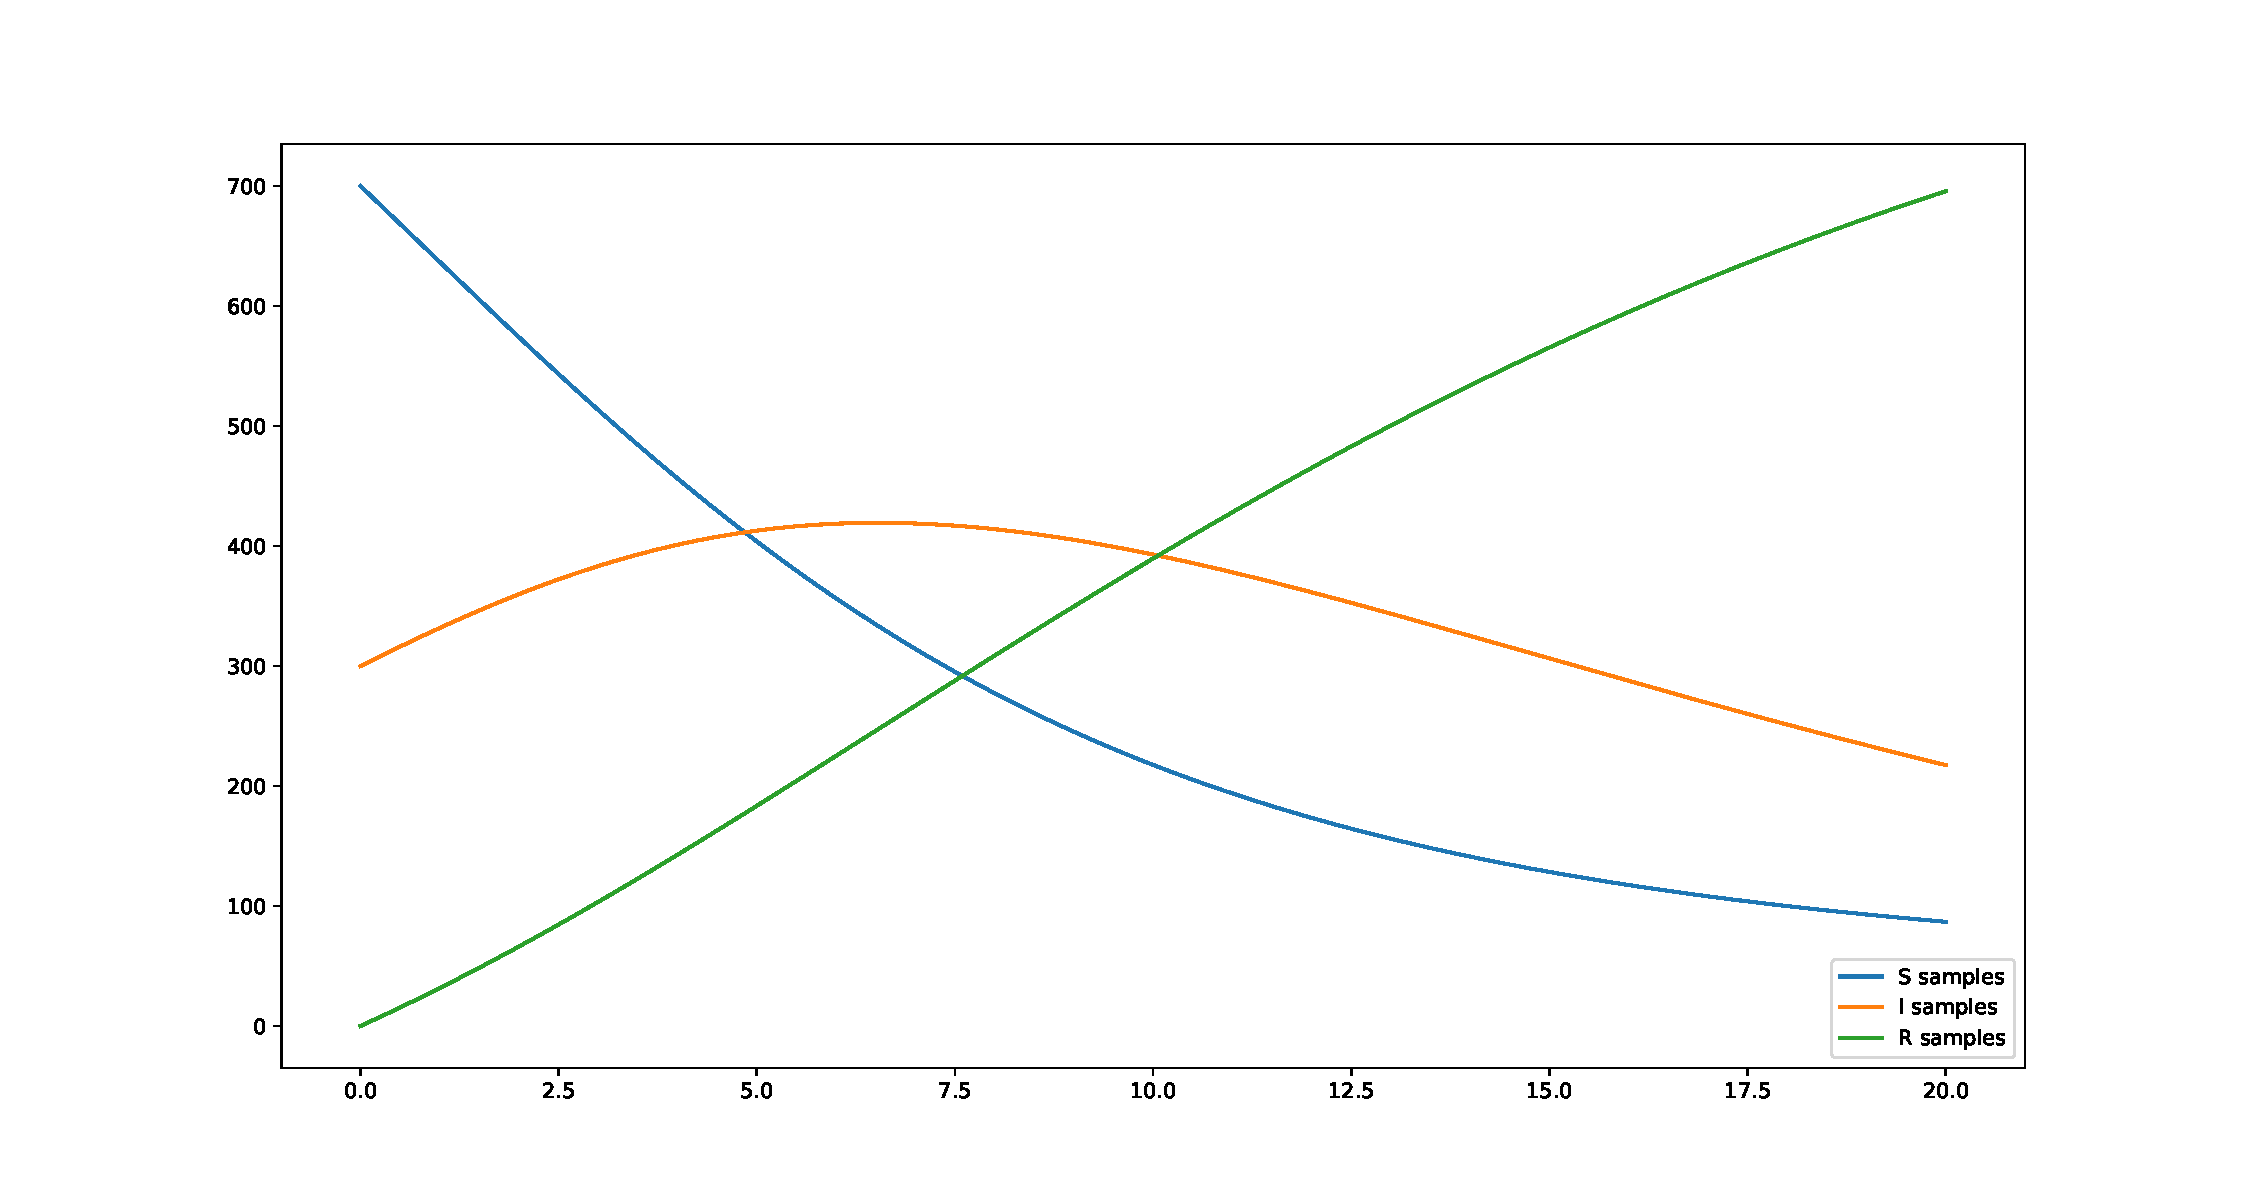
\includegraphics[width=\textwidth]{"figures/SIR.pdf"}
    \caption{modelo SIR con $a = 0.3$, $b = 0.1$.}
    \label{fig:SIR}
\end{figure}

Cuando se tienen los datos de la forma $\{(t_i, y_i), i=1, \dots, n\}$ generados por la integración del modelo, se le agregan distintos valores de ruido a los puntos. A cada muestra $y_i$ se le agrega un valor de ruido utilizando la fórmula:

$$y_{i_{noise}} = y_i + y_i * max\_noise * random\_standard\_normal(),$$

donde $random\_standard\_normal()$ es una función que genera valores aleatorios normales, independientes, con media 0 y varianza 1. $Max\_noise$ es un parámetro con mínimo valor $0$ y máximo $1$ que define el ``ruido  máximo'' que se le agrega a cada muestra. Se puede ver el parámetro $max\_noise$ como el \% máximo del valor de cada muestra que se puede agregar como ruido. Durante los distintos experimentos se utilizaron como máximo ruido los valores de 0\%, 5\% o 10\%.

Por ejemplo, si se agrega ruido a los datos obtenidos de la integración del sistema SIR utilizando el parámetro $max\_noise$ con valor $0.1$, se tendrían las curvas que aparecen en la imagen \ref{fig:SIR_with_noise} de la página \pageref{fig:SIR_with_noise}.

\begin{figure}[h]
    \centering
    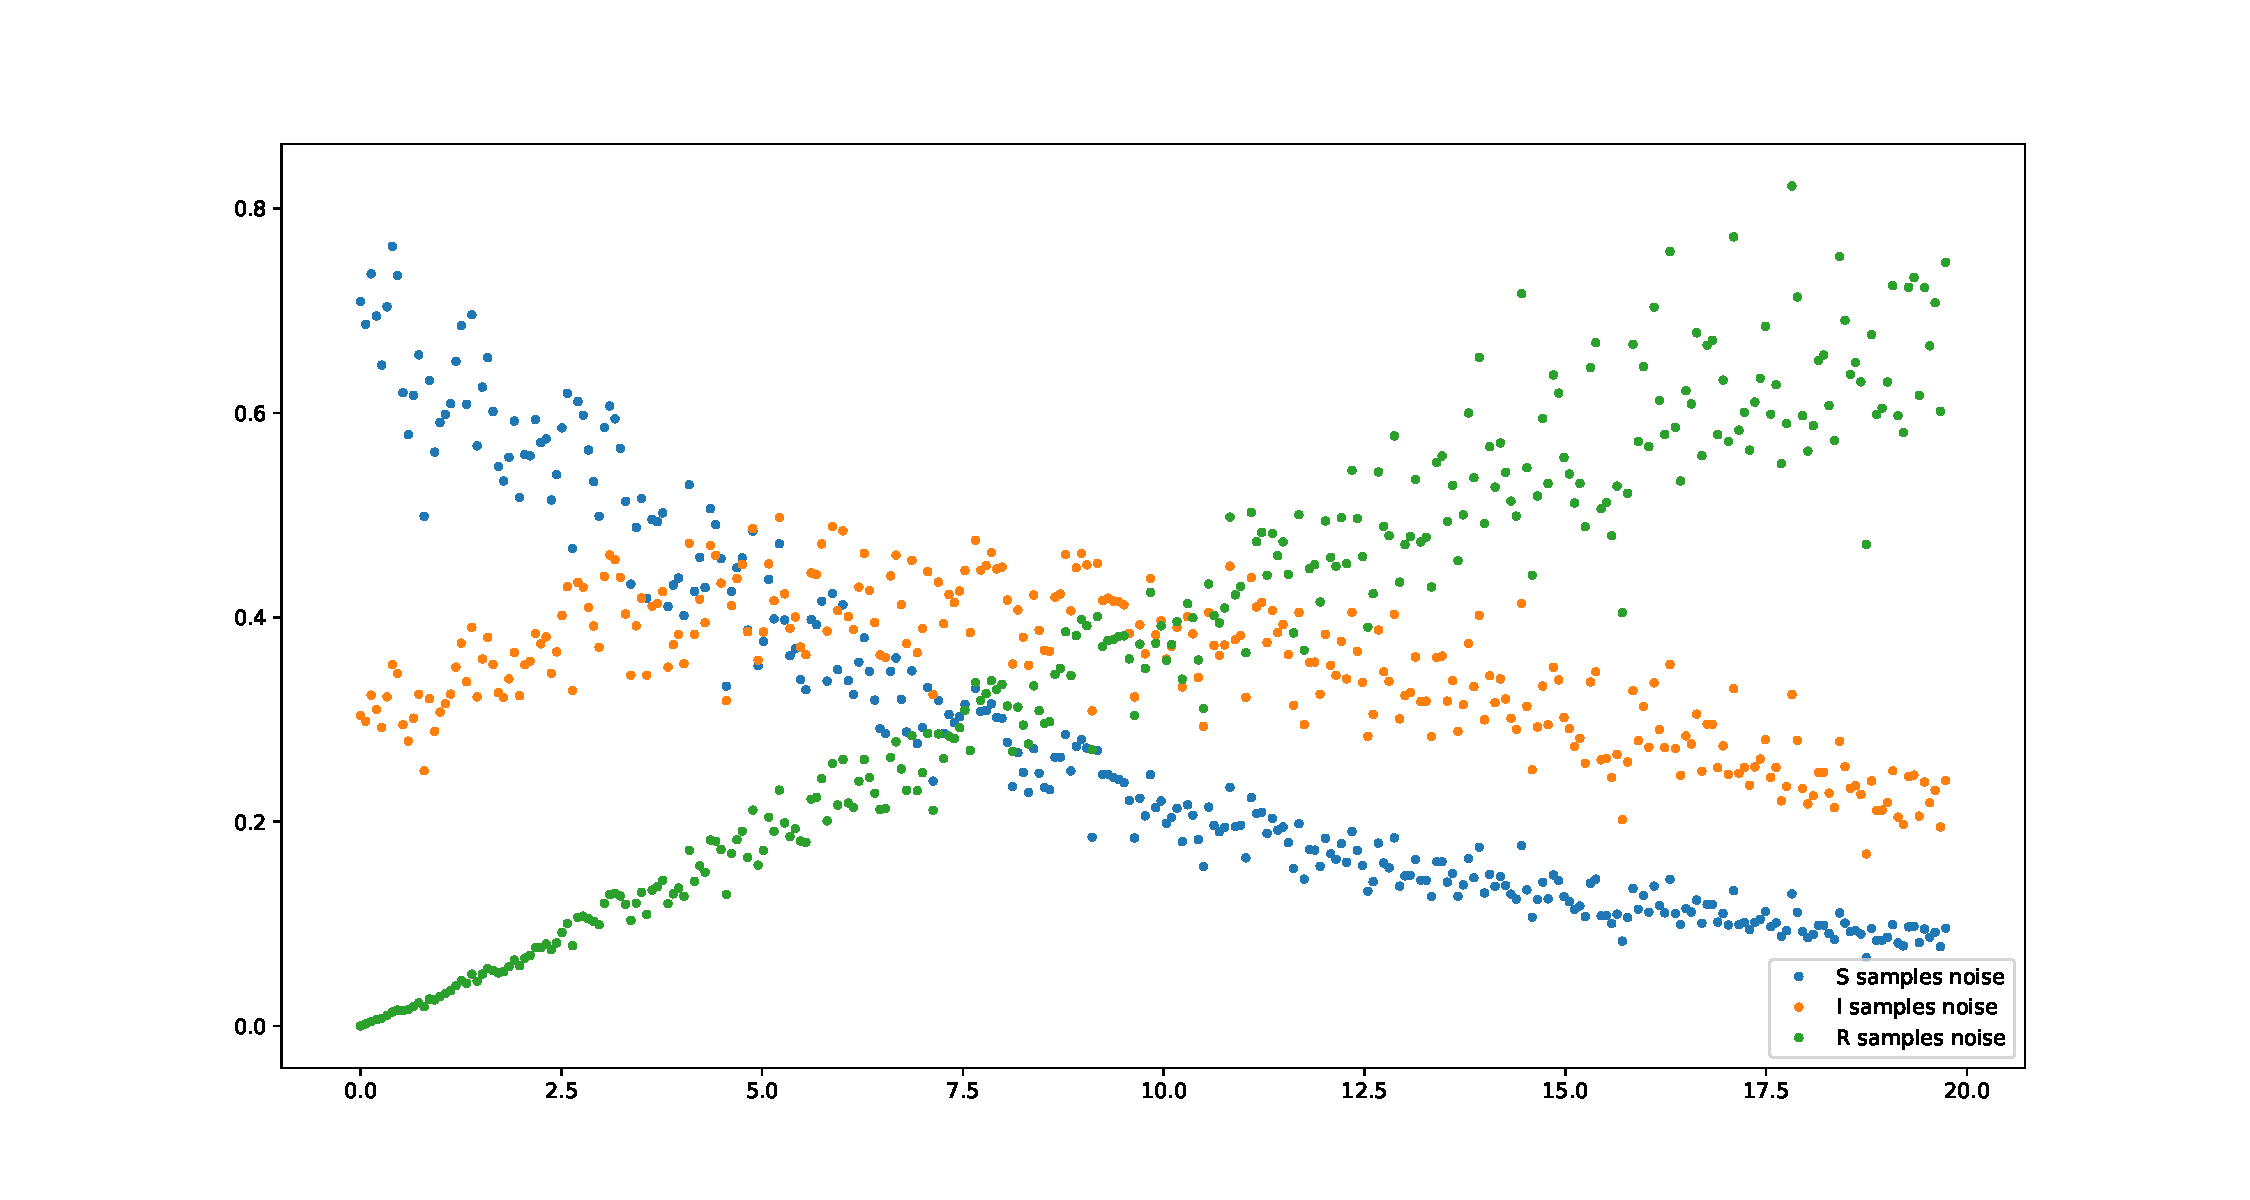
\includegraphics[width=\textwidth]{"figures/SIR_with_noise.pdf"}
    \caption{modelo SIR con $a = 0.3$, $b = 0.1$ y $max\_noise = 0.1$.}
    \label{fig:SIR_with_noise}
\end{figure}

Cuando el valor de $max\_noise$ es mayor que 0, se usa un spline de suavizado para eliminar el ruido. El valor del parámetro de suavizado en el spline se varía para cada una de las variables. Por ejemplo, si se utiliza un spline de suavizado cúbico en los datos con ruido del sistema SIR se obtendrían las curvas que aparecen en la imagen \ref{fig:SIR_noise_with_spline} de la página \pageref{fig:SIR_noise_with_spline}.

\begin{figure}[h]
    \centering
    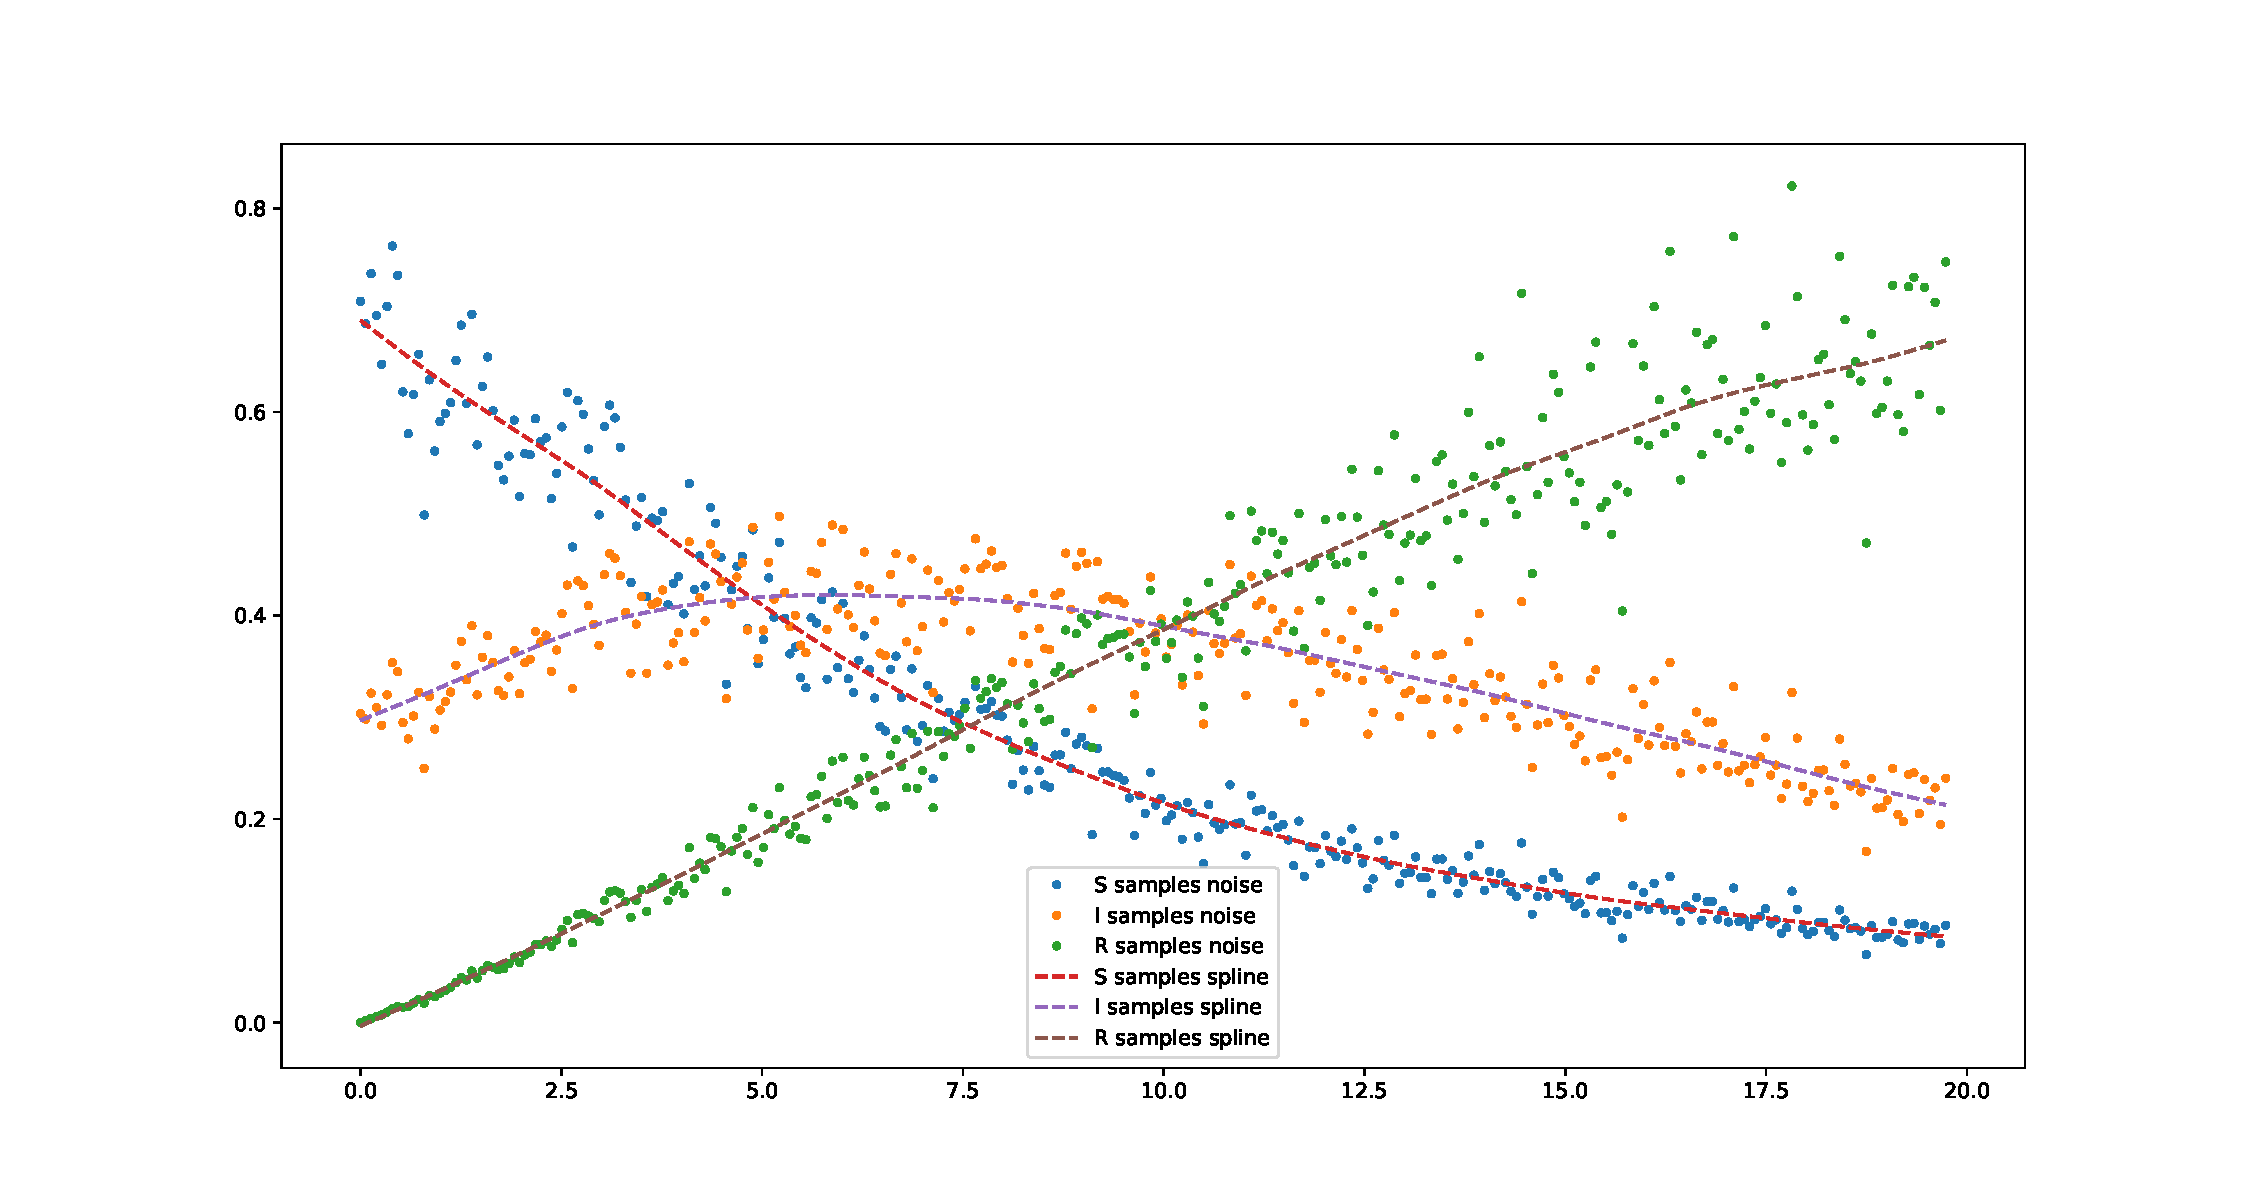
\includegraphics[width=\textwidth]{"figures/SIR_noise_with_spline.pdf"}
    \caption{modelo SIR con $a = 0.3$, $b = 0.1$, $max\_noise = 0.1$ y smoothing-spline con valor de suavizado de $0.1$.}
    \label{fig:SIR_noise_with_spline}
\end{figure}

Una vez que se tiene el spline de suavizado, se puede aproximar el valor de la función $y_i$, evaluando el spline correspondiente a el valor $t_i$. Como lo que se busca es generar un conjunto de datos de la forma:

$$\{(t_i, y_i, y'_i), i=1, \dots, n\},$$

para obtener $f(t_i, y_i)$ mediante el uso de la regresión simbólica, se puede generar una aproximación del valor de $y'_i$ utilizando la primera derivada del spline. Si el valor de $max\_noise$ es igual a 0, se aproxima el valor de $y'_i$ mediante el método de diferencias finitas. Se realizaron un subconjunto de experimentos utilizando como derivada el valor del modelo original $y'_i = f(t_i, y_i)$ para comprobar cuánto influye en el resultado de la regresión simbólica la aproximación de $y'_i$ mediante el método de diferencias finitas.

En las siguientes secciones se presentan los experimento en los que se utiliza la regresión simbólica para encontrar el sistema de ecuaciones diferenciales lineales con respecto a los parámetros a partir de un conjunto de datos generado. Se utilizaron en total 5 modelos para la generación de los disintos conjuntos de datos que fueron el sistema de lotka volterra \cite{Hoppensteadt:2006}, SIR \cite{weiss2013sir}, SIRD \cite{bailey1975mathematical}, SIQRD \cite{molter2021mathematical} y SVVEIR \cite{kuddus2021mathematical}.

\section{Experimentos realizados}\label{section:experiments}

Todos los sistemas de ecuaciones diferenciales seleccionados para los experimentos son sistemas lineales con respecto a los parámetros. La cantidad de ecuaciones en cada uno de los modelos es distinta. De cada modelo se muestra una tabla que contiene la media del valor de la función de ajuste a lo largo de las 30 ejecuciones del experimento así como el mínimo y máximo valor que alcanzó el error cuadrático medio.

Por cada experimento en el que se utiliza el modelo $f$, se genera un conjunto de datos $S$ de la forma $\{(t_i, y_i), i=1, \dots, n\}$ mediante la integración del modelo $f$. Luego se crea el conjunto de datos $y_{noise_{x\%}}$ resultantes de agregarle ruido al conjunto $S$ con $max\_noise=x$ y se define $y_{spline_{x\%}}$ como los datos resultantes de la aproximación de la función $y$ a partir de los datos $y_{noise_{x\%}}$. Con todos estos datos se genera el sistema $\hat{f}$ utilizando la regresión simbólica. Se define el conjunto de datos $y_{sr_{x\%}}$ como los datos generados por la integración del sistema encontrado en la regresión simbólica.

% Lo del PSO no se utilizará ahora
% Además se tiene el sistema $f_{pso}$ como el resultado de aplicar el método $PSO$ \cite{p-pso-6} utilizando el conjunto $S$.

De todos los experimentos en los que se utiliza el modelo $f$ solo se tuvieron en cuenta en los resultados un subconjunto de los 30 experimentos realizado. Si en algún momento el método \texttt{integrate.odeint} de la biblioteca \emph{scipy}, que se utiliza para la integración de un sistema de ecuaciones diferenciales, lanza una advertencia el experimento se desecha. Esta cantidad que se tiene en cuenta se define en la fila ``cantidad de sistemas'' de la tabla de resultados con la forma \ref{table:experiment_form} que aparece en la página \pageref{table:experiment_form}.

\begin{table}
    \centering
    \caption{Estructura de tabla de resultados.}
    \begin{tabular}{|c|c|}
        \hline
                             & \textbf{ruido de x\%}                                                \\
        \hline
        cantidad de sistemas & $m$                                                                  \\
        \hline
        original             & $\frac{\frac{\sum_{i=1}^n (y_i-y_{sr_{x\%}})^2}{n}}{m}$              \\
        \hline
        original con ruido   & $\frac{\frac{\sum_{i=1}^n (y_{noise_{x\%}}-y_{sr_{x\%}})^2}{n}}{m}$  \\
        \hline
        spline               & $\frac{\frac{\sum_{i=1}^n (y_{spline_{x\%}}-y_{sr_{x\%}})^2}{n}}{m}$ \\
        \hline
    \end{tabular}
    \label{table:experiment_form}
\end{table}

A continuación se muestra el experimento realizado a partir de la generación de los datos utlizando el sistema Lotka-Volterra.

\subsection{Lotka-Volterra}

El modelo de Lotka-Volterra es un sistema utilizado para describir las interacciones entre dos especies, una como depredador y otra como presa \cite{Hoppensteadt:2006}. La población de cada especie cambia a través del tiempo de acuerdo al sistema de ecuaciones diferenciales:

\begin{align*}
    X' & = X (a - b Y)   \\
    Y' & = -Y (c - d X).
\end{align*}

Se utilizaron como valores de los parámetros $a = 0.04$, $b = 0.0005$, $c = 0.2$ y $d = 0.004$ con punto inicial $(20, 20)$ y se integró en el intervalo $0 \leq t \leq 300$ para obtener los datos que aparecen en la figura \ref{fig:lotka_volterra} de la página \pageref{fig:lotka_volterra}. Del conjunto de puntos se seleccionaron 300 muestras como datos para el método de regresión simbólica.

\begin{figure}[h]
    \centering
    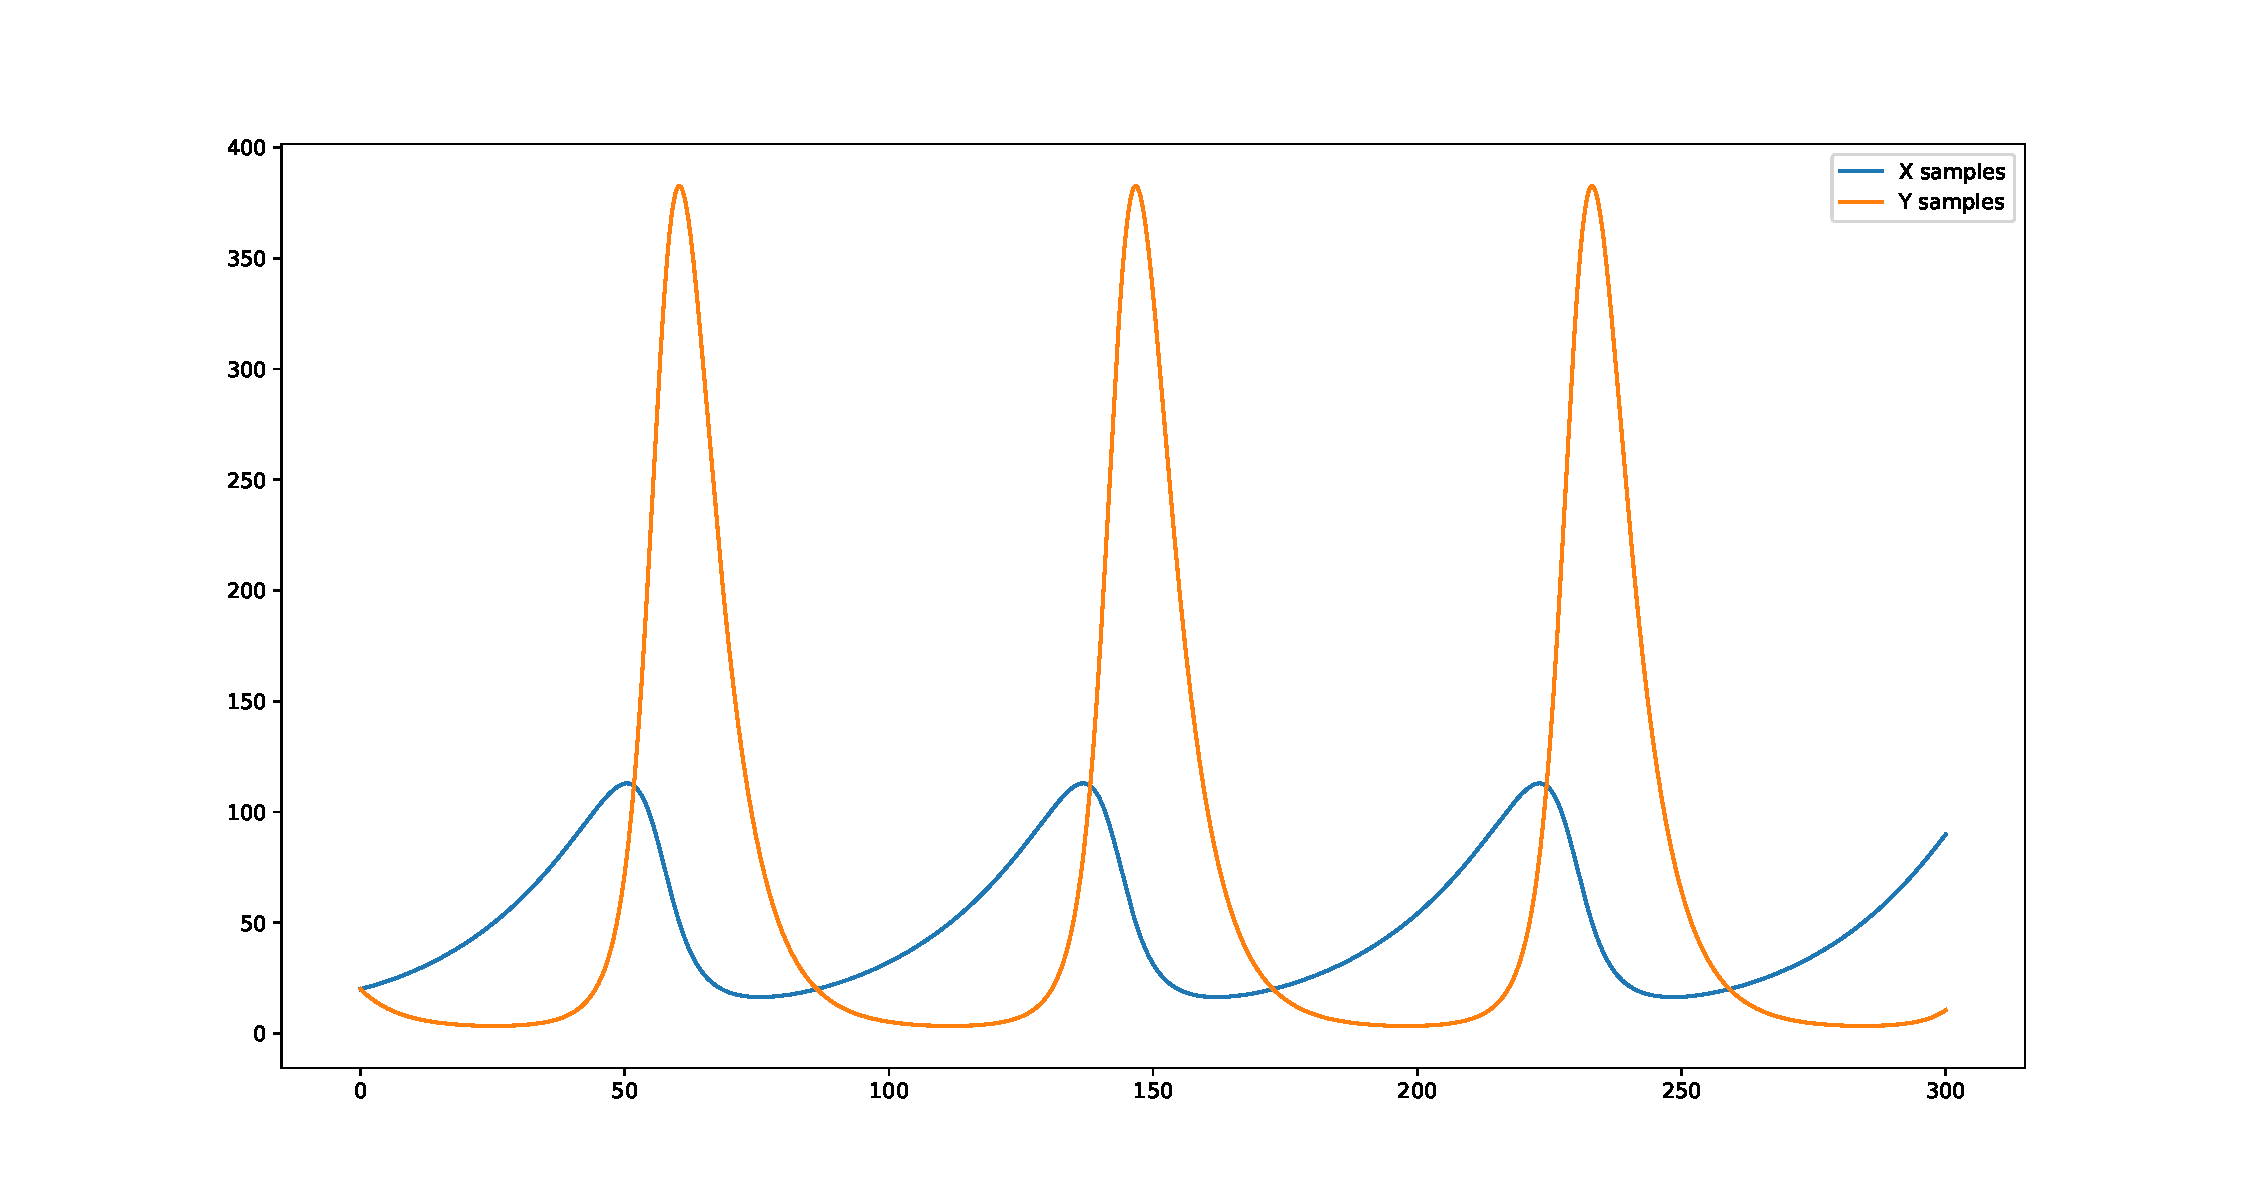
\includegraphics[width=\textwidth]{"figures/lotka_volterra.pdf"}
    \caption{modelo Lotka Volterra con $a = 0.04$, $b = 0.0005$, $c = 0.2$ y $d = 0.004$.}
    \label{fig:lotka_volterra}
\end{figure}

Los resultados que se obtienen durante las 30 ejecuciones del experimento aparecen en la tablas \ref{table:experiment_lotka_volterra}.

\begin{table}[!h]
    \centering
    \caption{Resultados que se obtienen en el modelo Lotka-Volterra.}

    \begin{tabular}{|c|c|c|c|}
        \hline
               & \textbf{ruido de 0\%} & \textbf{ruido de 5\%} & \textbf{ruido de 10\%} \\
        \hline
        media  & 0.74514               & 0.69138               & 0.84485                \\
        \hline
        mínimo & 0.28343               & 0.42189               & 0.54373                \\
        \hline
        máximo & 0.97944               & 1.11027               & 1.68603                \\
        \hline
    \end{tabular}

    \begin{tabular}{|c|c|c|c|c|c|}
        \hline
                             & \textbf{ruido de 0\%} & \textbf{ruido de 5\%} & \textbf{ruido de 10\%} \\
        \hline
        cantidad de sistemas & 30                    & 26                    & 24                     \\
        \hline
        original             & 17.01575              & 51.55822              & 49.92078               \\
        \hline
        original con ruido   & 17.01575              & 51.61296              & 50.18857               \\
        \hline
        spline               & 17.01575              & 51.23005              & 49.59158               \\
        \hline
    \end{tabular}

    \label{table:experiment_lotka_volterra}
\end{table}

Durante la realización de los experimentos el modelo de lotka-volterra, la regresión simbólica encontró el sistema que generó los datos pero con otros parámetros en 21 ocasiones cuando no se utilizaba ruido en los datos, 13 veces cuando se utilizó un ruido máximo de 5\% y 6 veces cuando se utilizó un ruido máximo de 10\%. En las figuras \ref{fig:final_plot_LV_0.0} de la página \pageref{fig:final_plot_LV_0.0}, \ref{fig:final_plot_LV_0.05} de la página \pageref{fig:final_plot_LV_0.05} y \ref{fig:final_plot_LV_0.1} de la página \pageref{fig:final_plot_LV_0.1} se pueden ver los datos originales comparados con los datos obtenidos del mejor resultado generado por la regresión simbólica.

\begin{figure}[h]
    \centering
    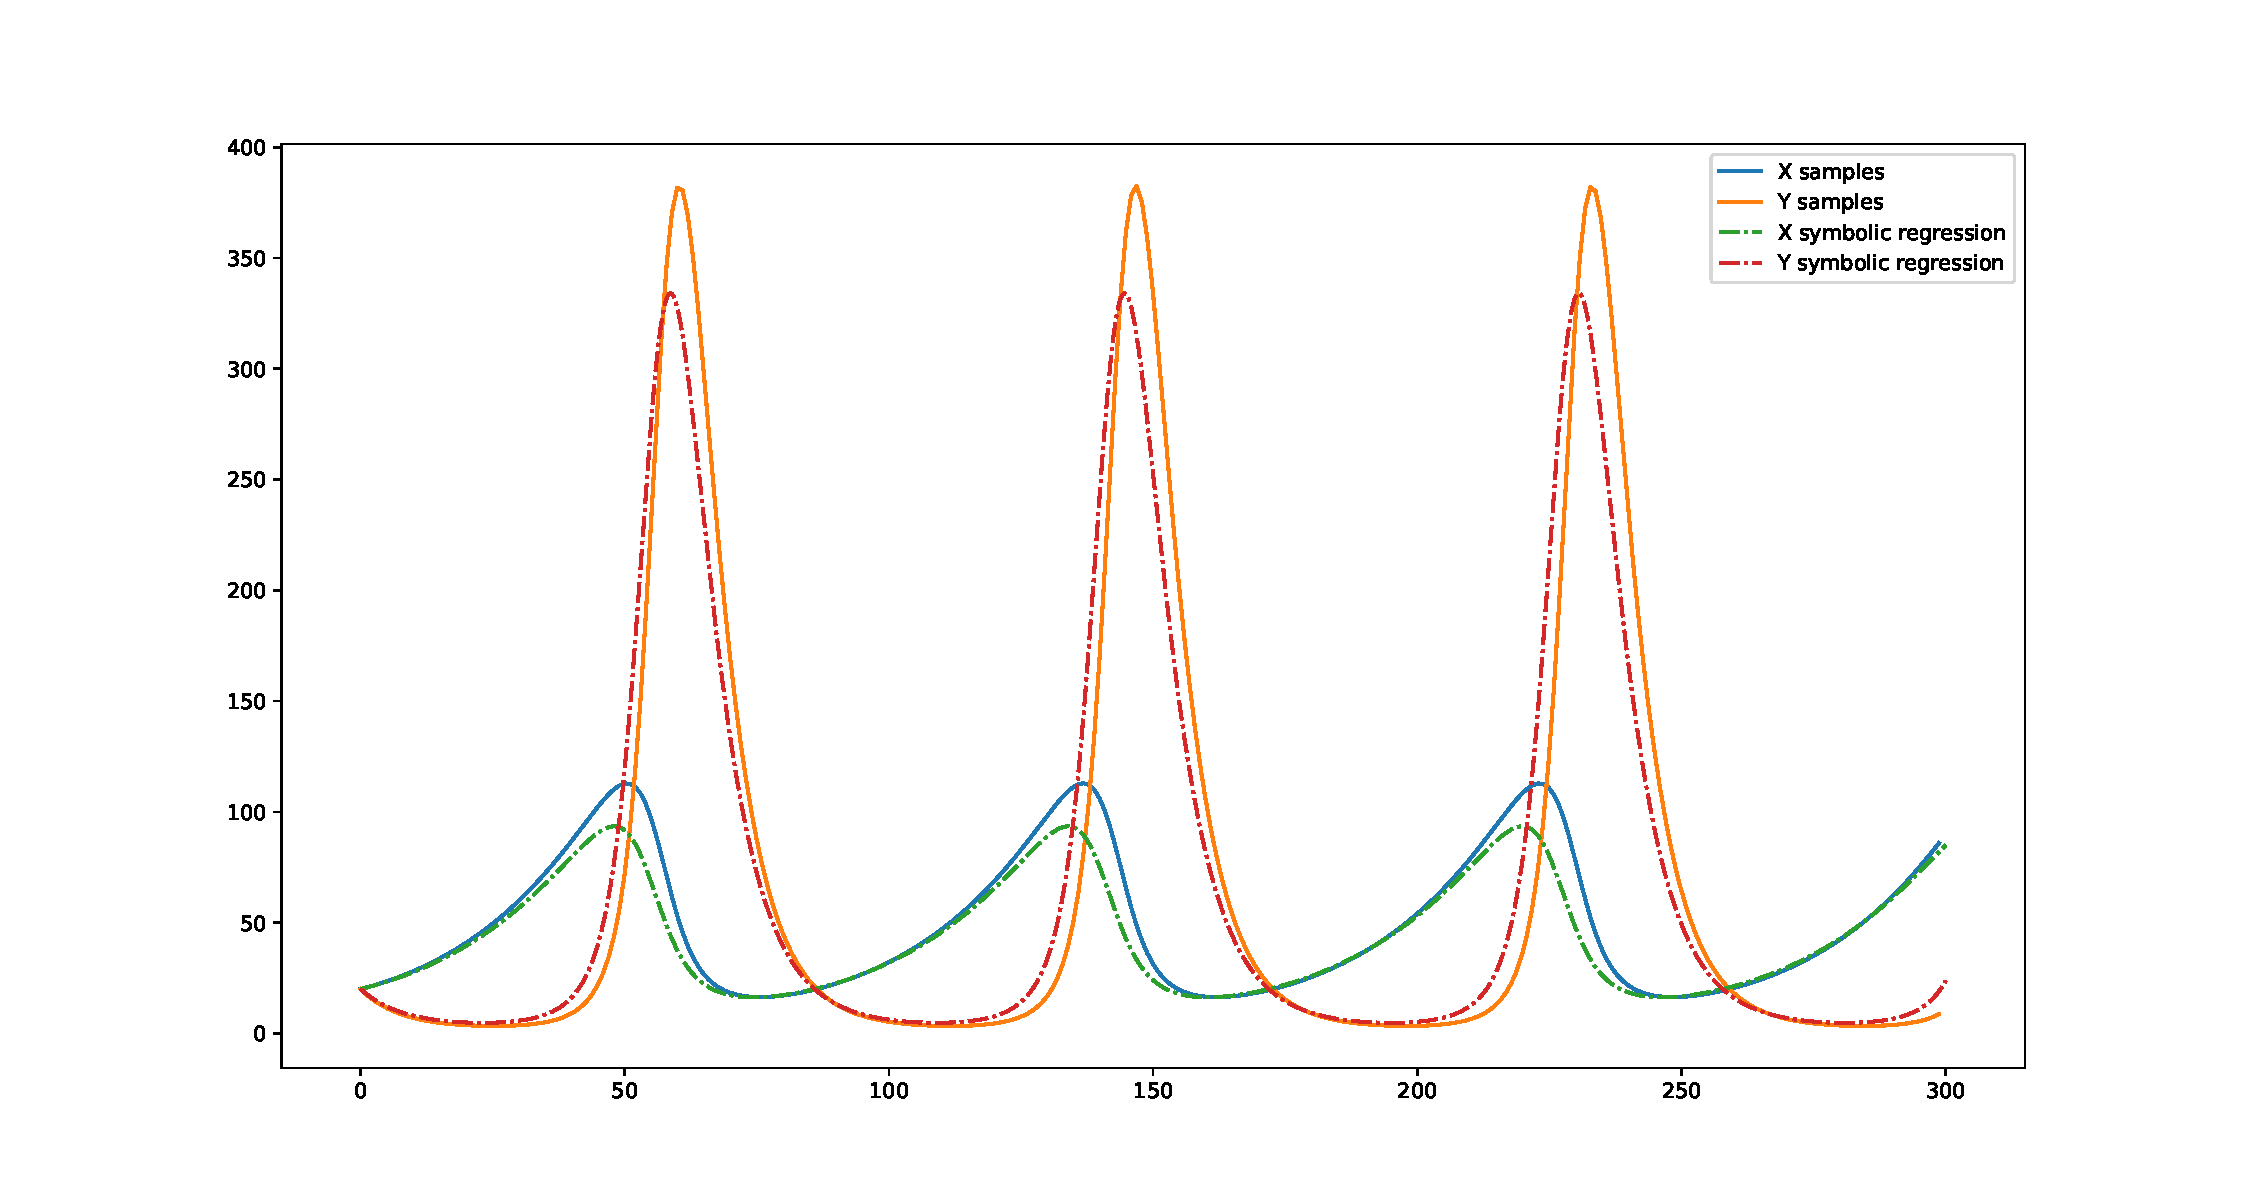
\includegraphics[width=\textwidth]{"figures/final_plot_LV_0.0.pdf"}
    \begin{align*}
        X' & = -0.0005 * (Y * X) + 0.03872 * X        \\
        Y' & = -0.00443 * (X * -(Y)) + 0.19573 * -(Y)
    \end{align*}
    \caption{Modelo resultante utilizando datos generados a partir del modelo lotka-volterra con ruido máximo de 0\%.
    }
    \label{fig:final_plot_LV_0.0}
\end{figure}

\begin{figure}[h]
    \centering
    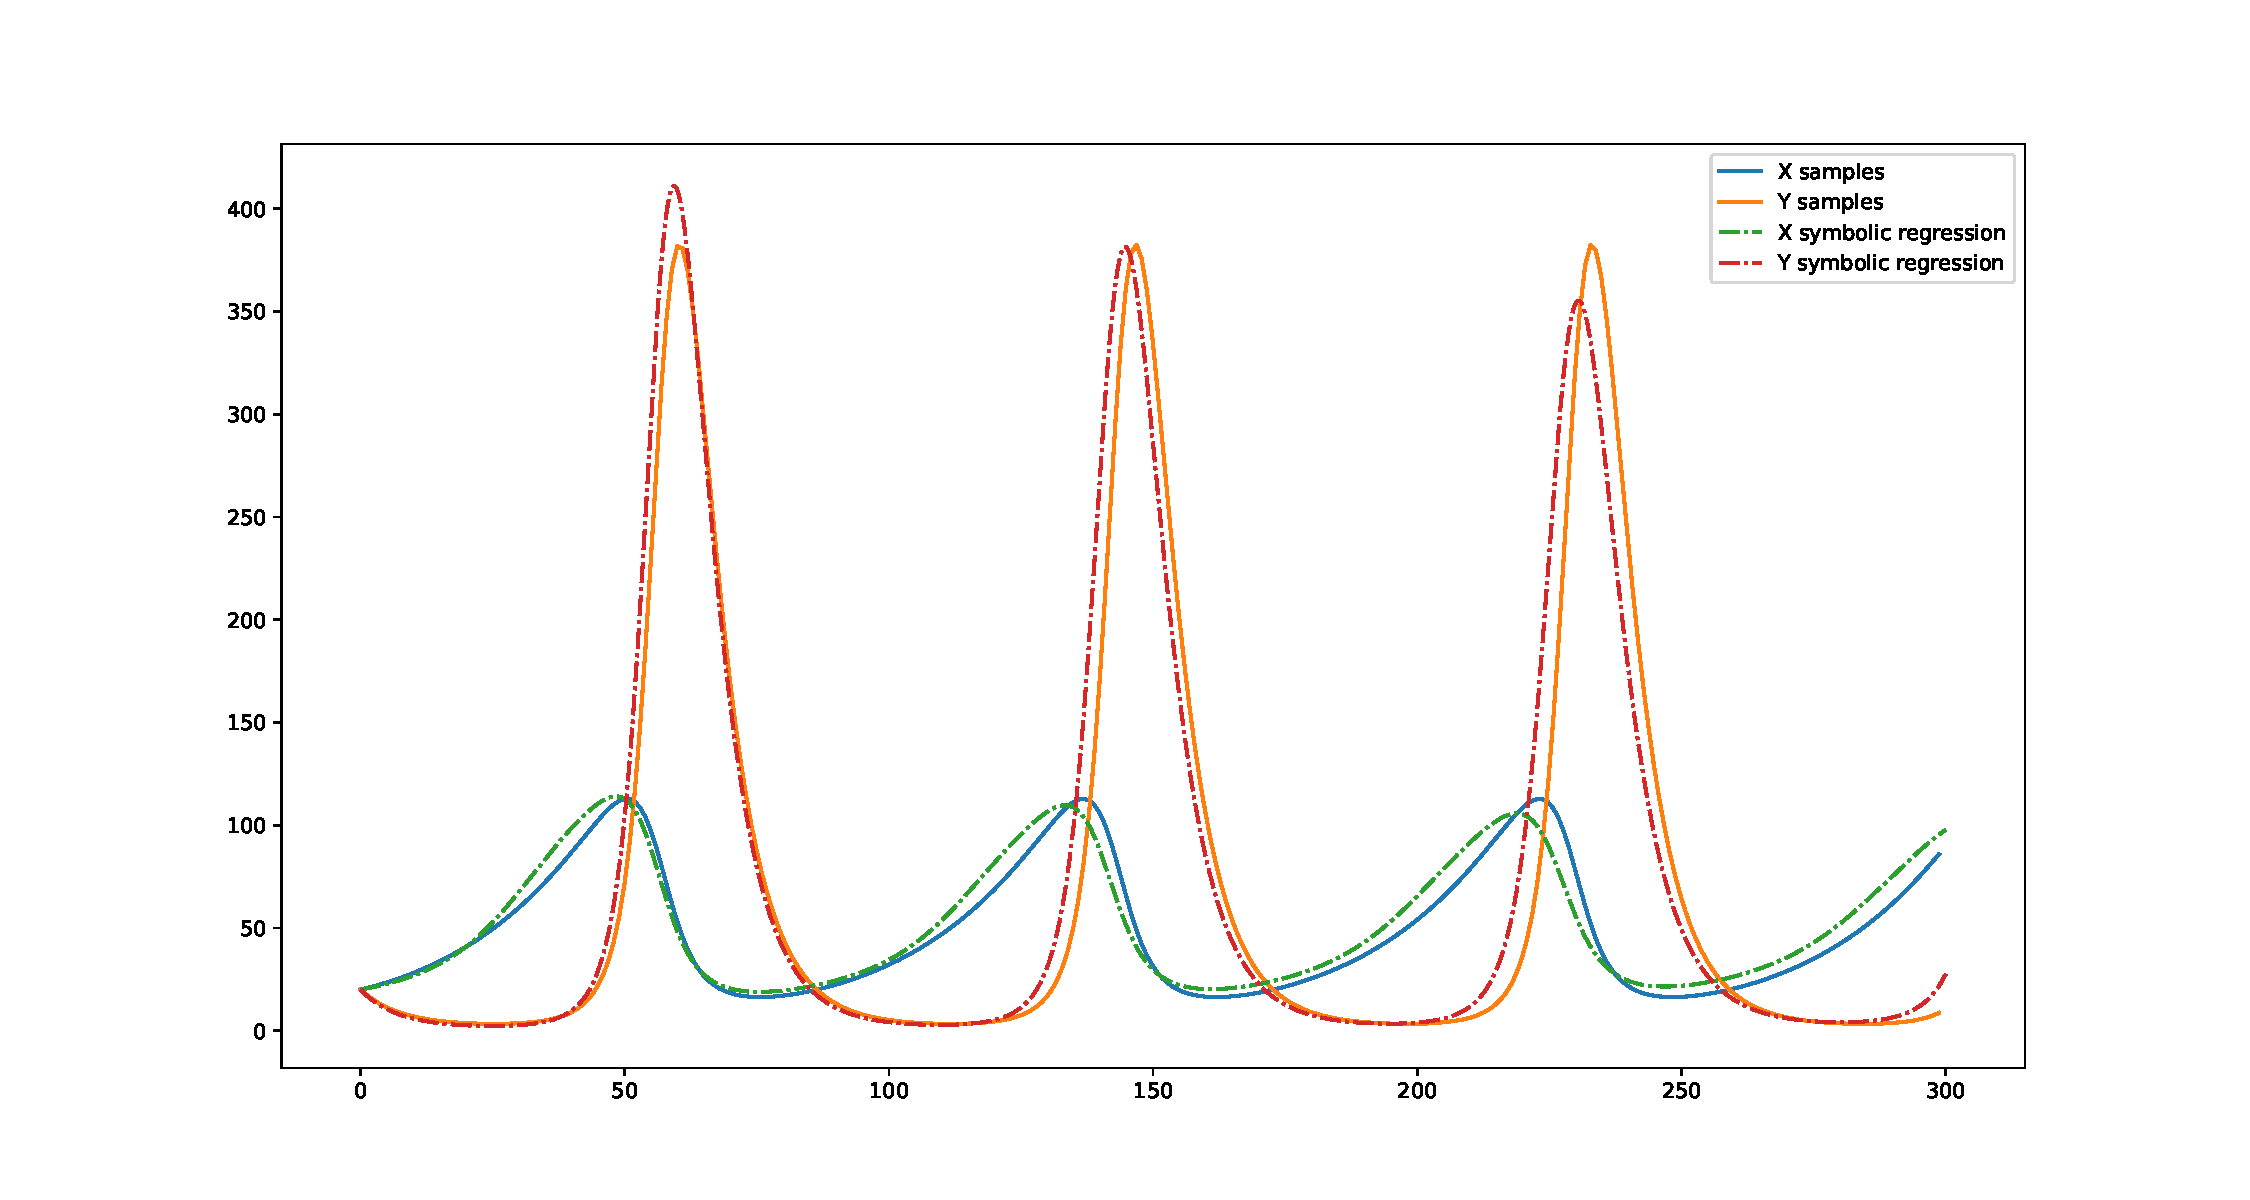
\includegraphics[width=\textwidth]{"figures/final_plot_LV_0.05.pdf"}
    \begin{align*}
        X' & = 0.06048 * ((Y + X) / Y) + 0.02512 * X -0.00039 * (Y * X) \\
        Y' & = 0.00416 * (X * Y) -0.21823 * Y
    \end{align*}
    \caption{Modelo resultante utilizando datos generados a partir del modelo lotka-volterra con ruido máximo de 5\%.}
    \label{fig:final_plot_LV_0.05}
\end{figure}

\begin{figure}[h]
    \centering
    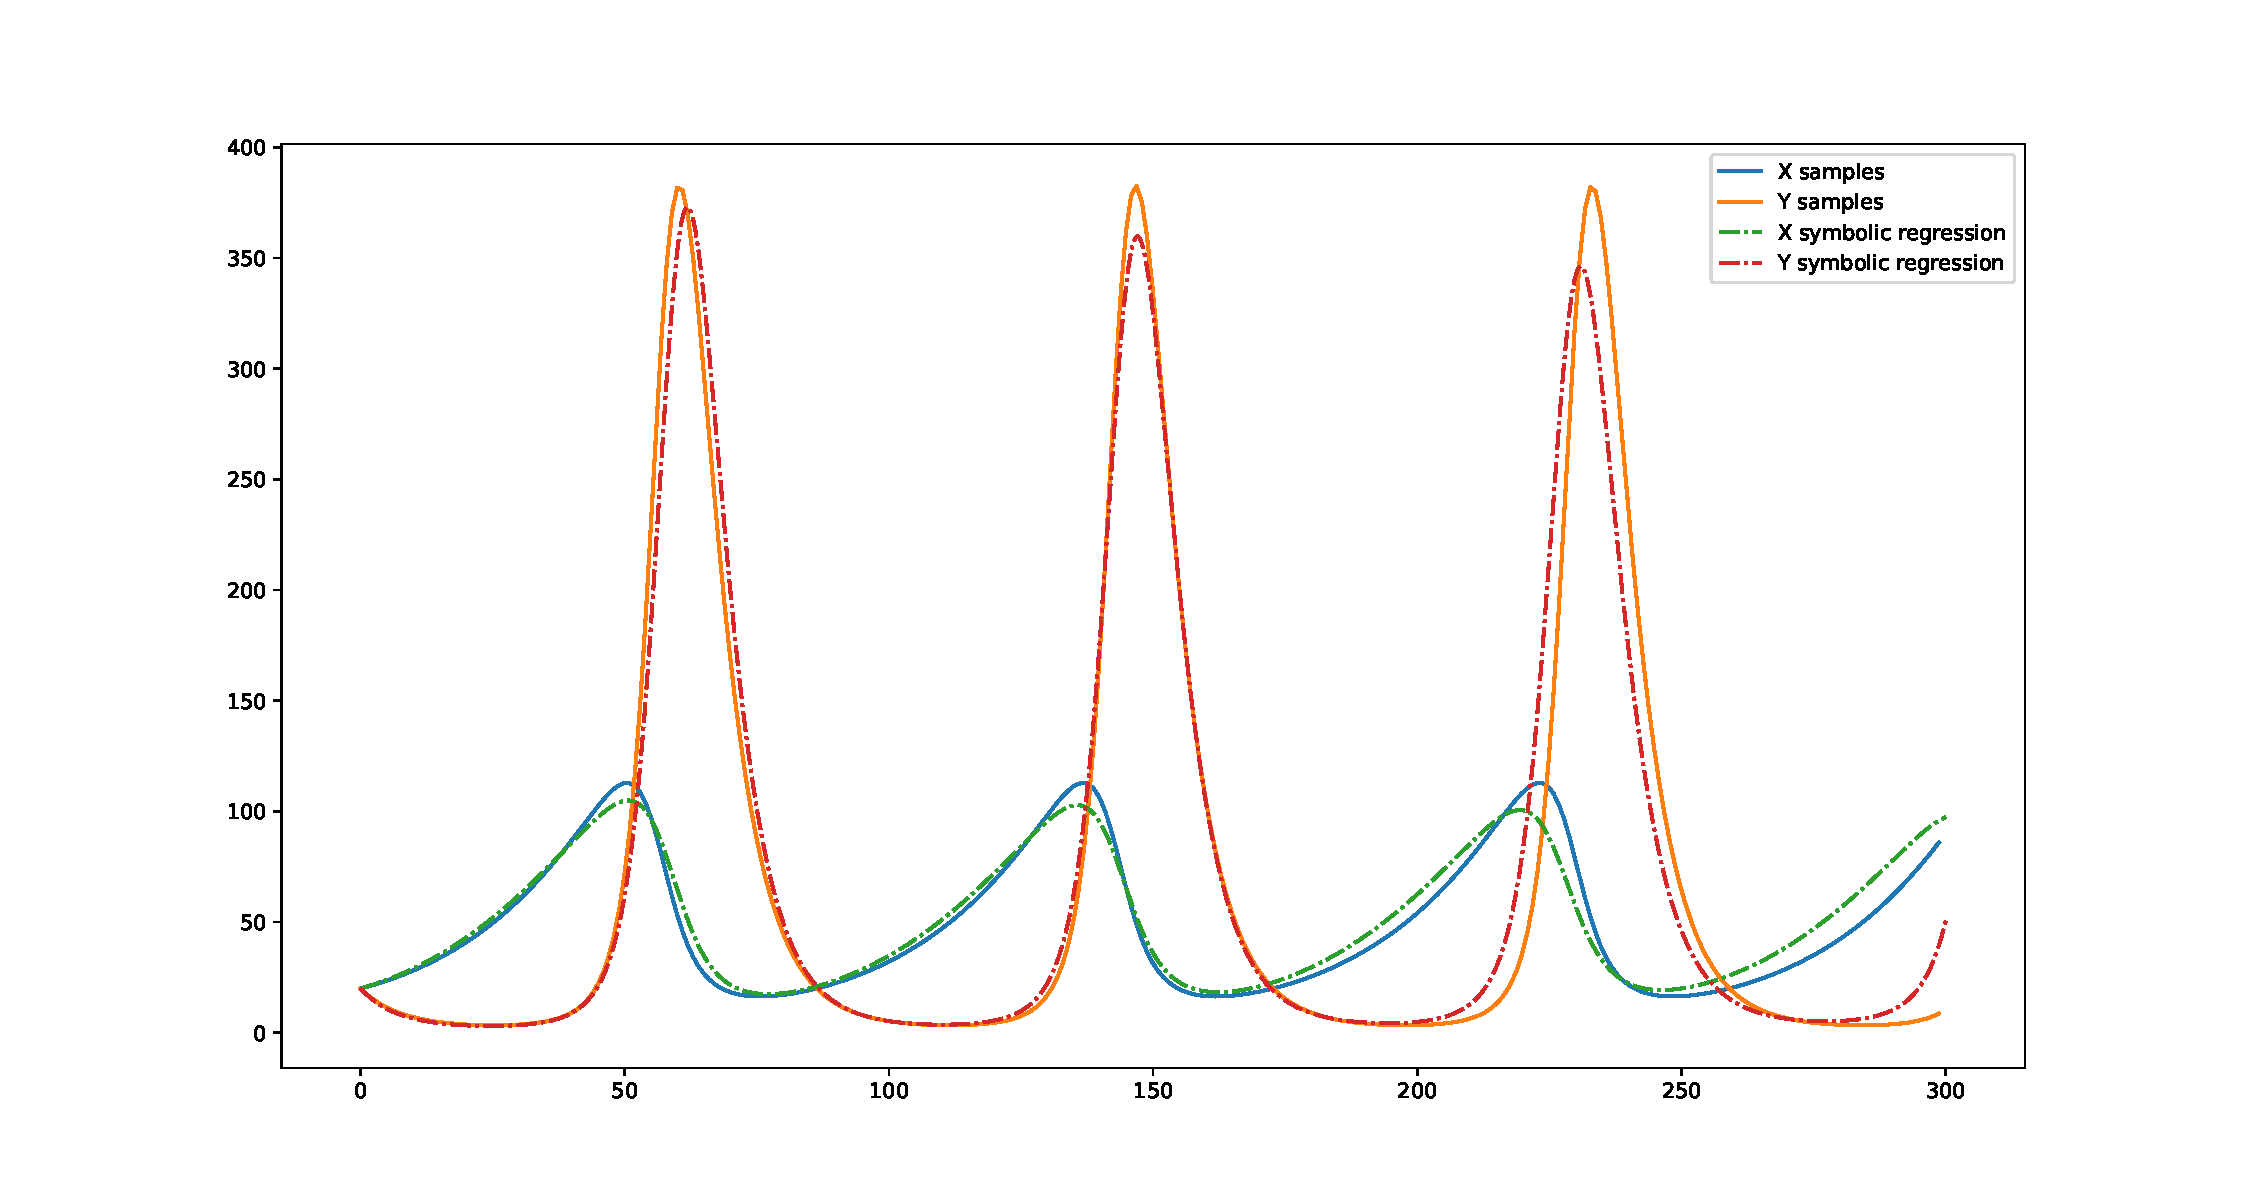
\includegraphics[width=\textwidth]{"figures/final_plot_LV_0.1.pdf"}
    \begin{align*}
        X' & = 0.04776 * X -0.00421 * Y -0.00018 * (X * (X + (Y + Y))) \\
        Y' & = 0.00424 * (Y * X) -0.21669 * Y
    \end{align*}
    \caption{Modelo resultante utilizando datos generados a partir del modelo lotka-volterra con ruido máximo de 10\%.}
    \label{fig:final_plot_LV_0.1}
\end{figure}


En el resto de experimentos realizados utilizando otros modelos, nunca se obtuvo como resultado de la regresión simbólica el modelo original que generó los datos pero se encuentran modelos que se aproximan a los datos.

Si en lugar de utilizar como aproximación de la derivada el método de diferencias finitas cuando los datos no poseen ruido, se utiliza el sistema original de Lotka-Volterra, se obtiene que la media del valor de la función de ajuste a lo largo de las 30 ejecuciones del experimento es $0.00721$. El valor máximo de la función de ajuste alcanzado fue de $0.21654$ y el mínimo de $6.35015e-16$, en este último la regresión simbólica obtuvo exactamente el sistema utilizado para generar los datos.


A continuación se muestra el experimento realizado a partir de la generación de los datos utilizando el sistema SIR.

\subsection{SIR}

El modelo SIR es un sistema que se utiliza para describir la transmisión de una enfermedad infecciosa causada por una bacteria, virus u hongos. \cite{weiss2013sir}. El sistema se define como:

\begin{align*}
    S' & = - aIS    \\
    I' & = aIS - bI \\
    R' & = bI,
\end{align*}

donde $S$ indica la cantidad de personas susceptibles, $I$ la cantidad de personas infectadas y $R$ la cantidad de personas recuperadas. Se utiliza el parámetro $a$ para indicar el índice de transmisión y $b$ el índice de recuperación de la enfermedad.

Se utilizaron como valores de los parámetros $a = 0.0003$ y $b = 0.1$ con punto inicial $(0.7, 0.3, 0)$ y se integró en el intervalo $0 \leq t \leq 20$ para obtener los datos que aparecen en la imagen \ref{fig:SIR} de la página \pageref{fig:SIR}. Del conjunto de puntos se seleccionaron 300 muestras como datos para el método de regresión simbólica.

Los resultados que se obtienen durante las 30 ejecuciones del experimento, utilizando solamente en cada ecuación las variables permitidas según el modelo, aparecen en la tabla \ref{table:experiment_SIR} de la página \pageref{table:experiment_SIR}. Si se permite cualquier variable del modelo en cualquier ecuación del sistema se obtienen los datos que aparecen en la tabla \ref{table:experiment_SIR_all} de la página \pageref{table:experiment_SIR_all}.

\begin{table}[!h]
    \centering
    \caption{Resultados que se obtienen en el modelo SIR restringiendo las variables que aparecen en cada ecuación.}
    \begin{tabular}{|c|c|c|c|}
        \hline
               & \textbf{ruido de 0\%} & \textbf{ruido de 5\%} & \textbf{ruido de 10\%} \\
        \hline
        media  & 2e-05                 & 0.0012                & 0.00233                \\
        \hline
        mínimo & 2e-05                 & 0.00078               & 0.00144                \\
        \hline
        máximo & 2e-05                 & 0.00195               & 0.00386                \\
        \hline
    \end{tabular}

    \begin{tabular}{|c|c|c|c|c|c|}
        \hline
                             & \textbf{ruido de 0\%} & \textbf{ruido de 5\%} & \textbf{ruido de 10\%} \\
        \hline
        cantidad de sistemas & 30                    & 29                    & 29                     \\
        \hline
        original             & 0.00066               & 0.01891               & 0.01744                \\
        \hline
        original con ruido   & 0.00066               & 0.02774               & 0.03472                \\
        \hline
        spline               & 0.00066               & 0.01873               & 0.0172                 \\
        \hline
    \end{tabular}
    \label{table:experiment_SIR}
\end{table}

\begin{table}[!h]
    \centering
    \caption{Resultados que se obtienen en el modelo SIR sin restringir las variables que aparecen en cada ecuación.}
    \begin{tabular}{|c|c|c|c|}
        \hline
               & \textbf{ruido de 0\%} & \textbf{ruido de 5\%} & \textbf{ruido de 10\%} \\
        \hline
        media  & 2e-05                 & 0.00121               & 0.00232                \\
        \hline
        mínimo & 0.0                   & 0.00079               & 0.00144                \\
        \hline
        máximo & 0.00023               & 0.00201               & 0.004                  \\
        \hline
    \end{tabular}

    \begin{tabular}{|c|c|c|c|c|c|}
        \hline
                             & \textbf{ruido de 0\%} & \textbf{ruido de 5\%} & \textbf{ruido de 10\%} \\
        \hline
        cantidad de sistemas & 30                    & 30                    & 29                     \\
        \hline
        original             & 0.00065               & 0.00547               & 0.01416                \\
        \hline
        original con ruido   & 0.00065               & 0.01465               & 0.03192                \\
        \hline
        spline               & 0.00065               & 0.0054                & 0.01394                \\
        \hline
    \end{tabular}
    \label{table:experiment_SIR_all}
\end{table}

En las figuras \ref{fig:final_plot_SIR_0.0} de la página \pageref{fig:final_plot_SIR_0.0}, \ref{fig:final_plot_SIR_0.05} de la página \pageref{fig:final_plot_SIR_0.05} y \ref{fig:final_plot_SIR_0.1} de la página \pageref{fig:final_plot_SIR_0.1} se pueden ver los datos originales comparados con los datos obtenidos del mejor resultado generado por la regresión simbólica restringiendo las variables que pueden existir en cada ecuación.

Durante la realización de los experimentos utilizando el modelo SIR nunca se obtuvo un sistema igual como resultado de la regresión simbólica. Pero el resultado ajustó los datos no importa la cantidad de ruido utilizado. Los datos que se obtienen de la integración del sistema resultante de la regresión simbólica se asemejan a los datos de la integración del sistema seleccionado para la realización del experimento.

\begin{figure}[h]
    \centering
    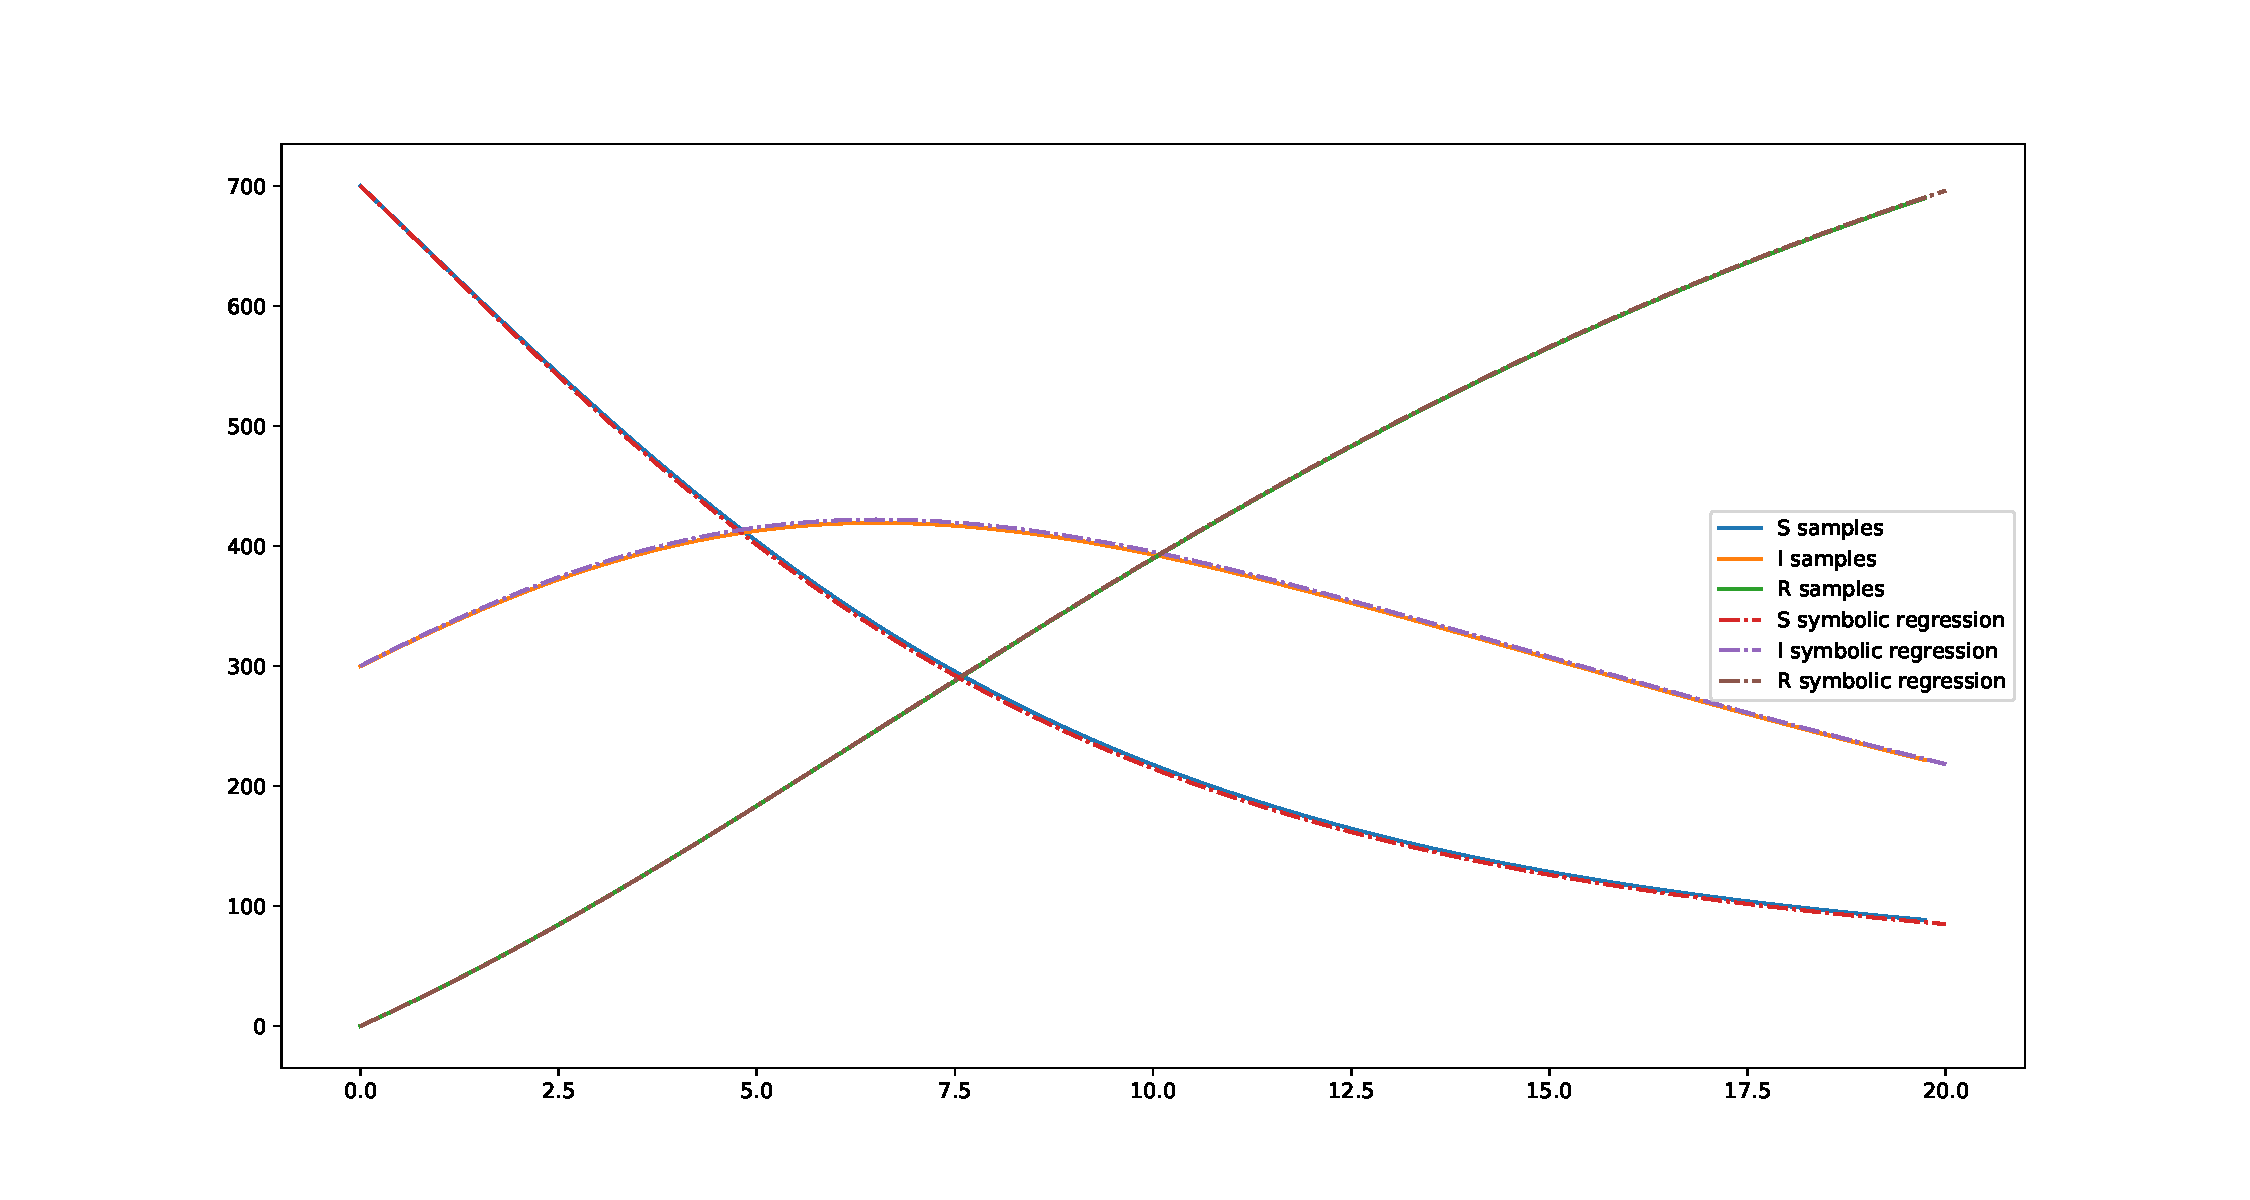
\includegraphics[width=\textwidth]{"figures/final_plot_SIR_0.0.pdf"}
    \begin{align*}
        S' & = -0.29801 * (S * I) + 0.00099 * (-(S) * S)         \\
        I' & = -0.396 * I + 0.29605 * (I + (I * S)) + 0.0011 * S \\
        R' & = 0.10033 * I -0.00013
    \end{align*}
    \caption{Modelo resultante utilizando datos generados a partir del modelo SIR con ruido máximo de 0\%.}
    \label{fig:final_plot_SIR_0.0}
\end{figure}

\begin{figure}[h]
    \centering
    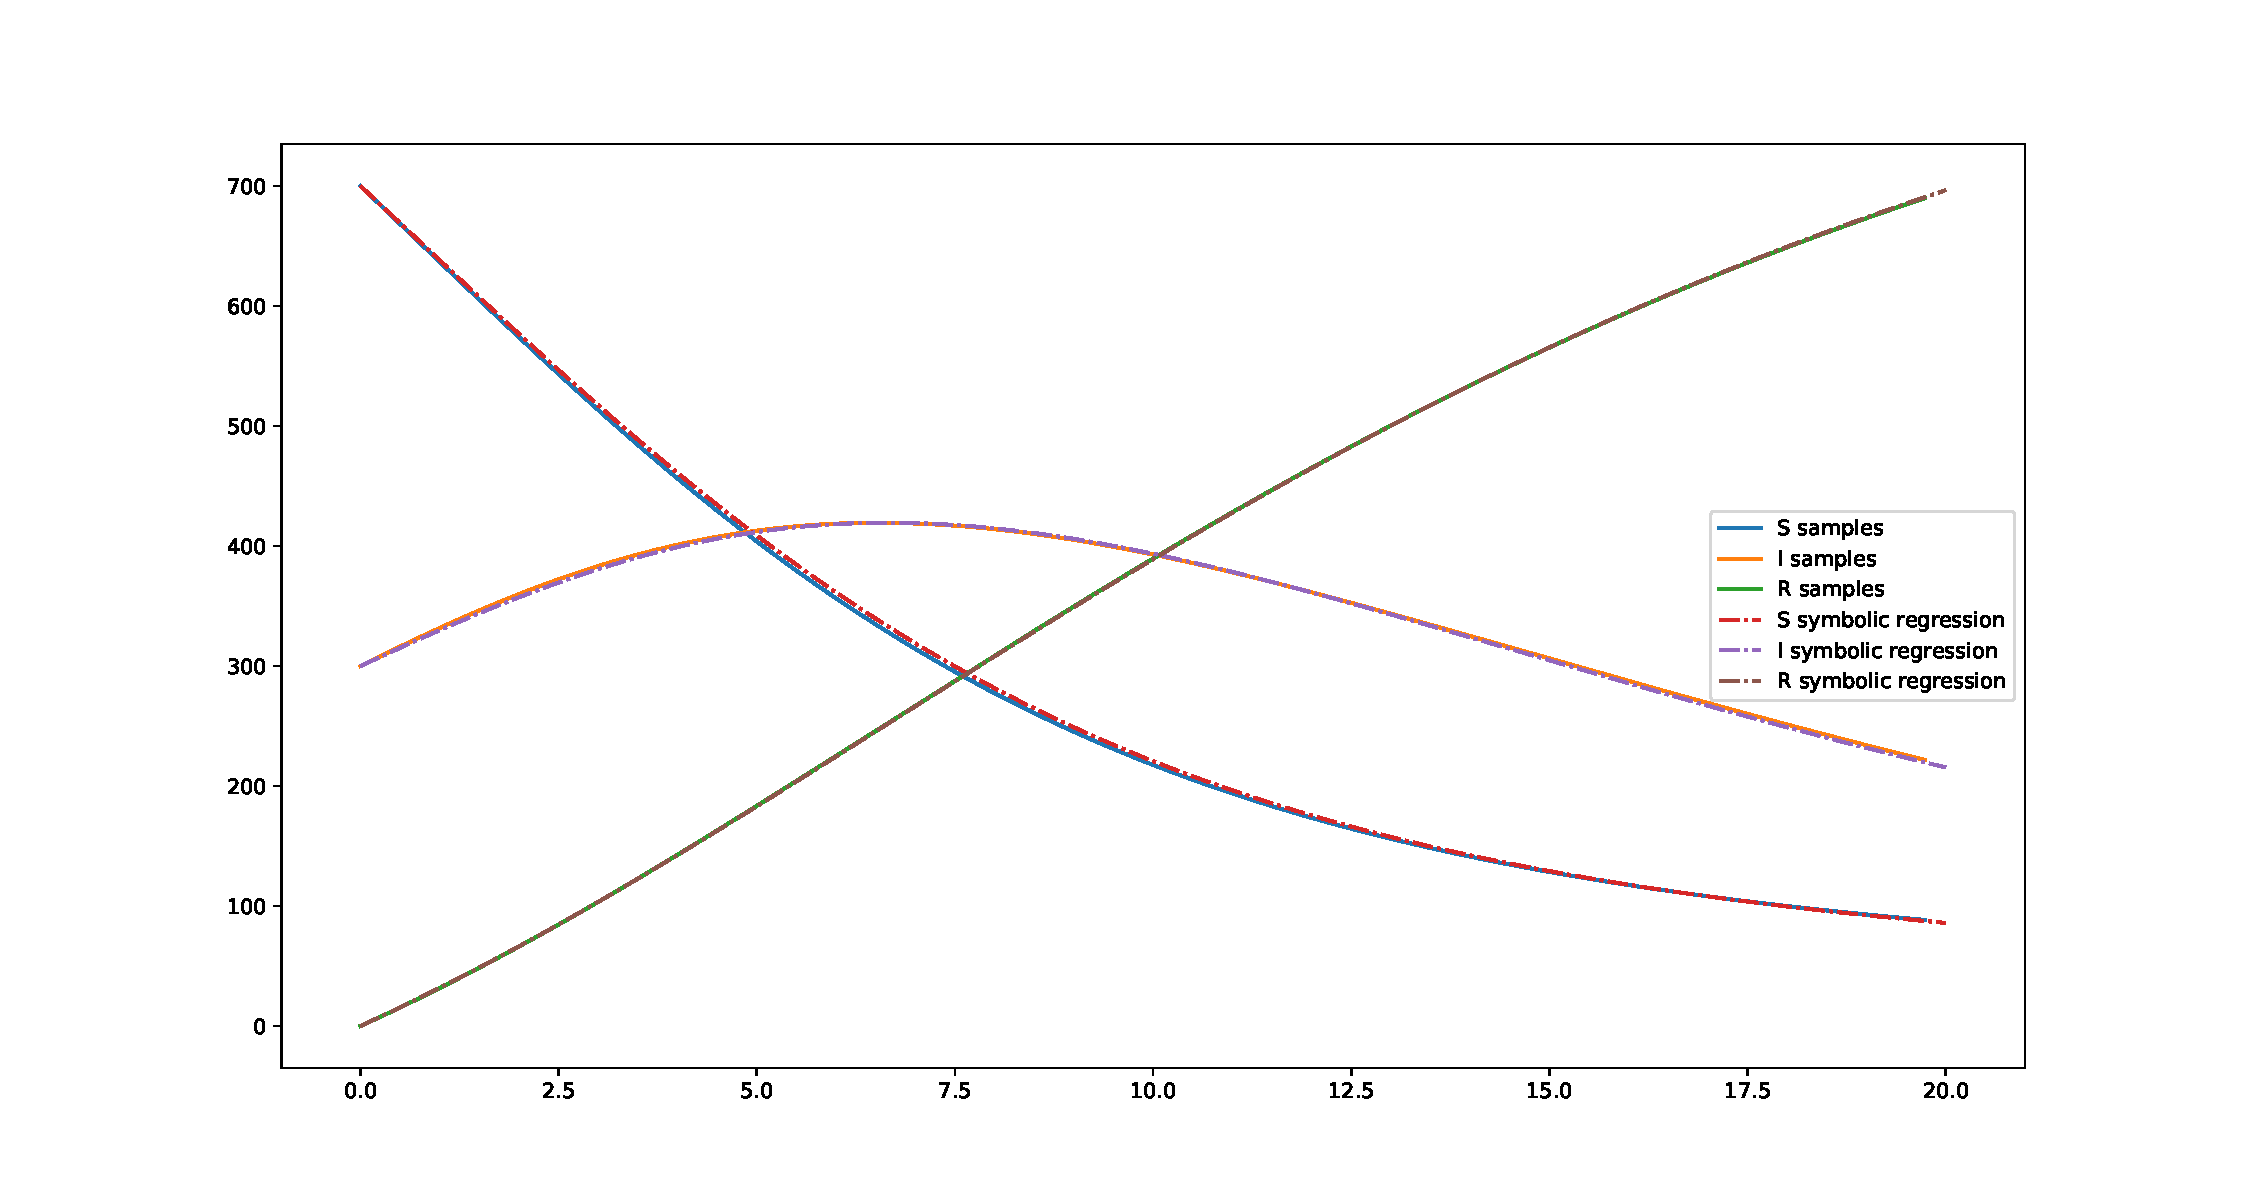
\includegraphics[width=\textwidth]{"figures/final_plot_SIR_0.05.pdf"}
    \begin{align*}
        S' & = 0.86088 * ((I * (I * I)) * S) + -0.00352 * -(-(I)) -0.06025 * S \\
        I' & = 0.12132 * (I * (S + I)) + -0.14216 * I + 0.06245 * S            \\
        R' & = 0.09928 * I
    \end{align*}
    \caption{Modelo resultante utilizando datos generados a partir del modelo SIR con ruido máximo de 5\%.}
    \label{fig:final_plot_SIR_0.05}
\end{figure}

\begin{figure}[h]
    \centering
    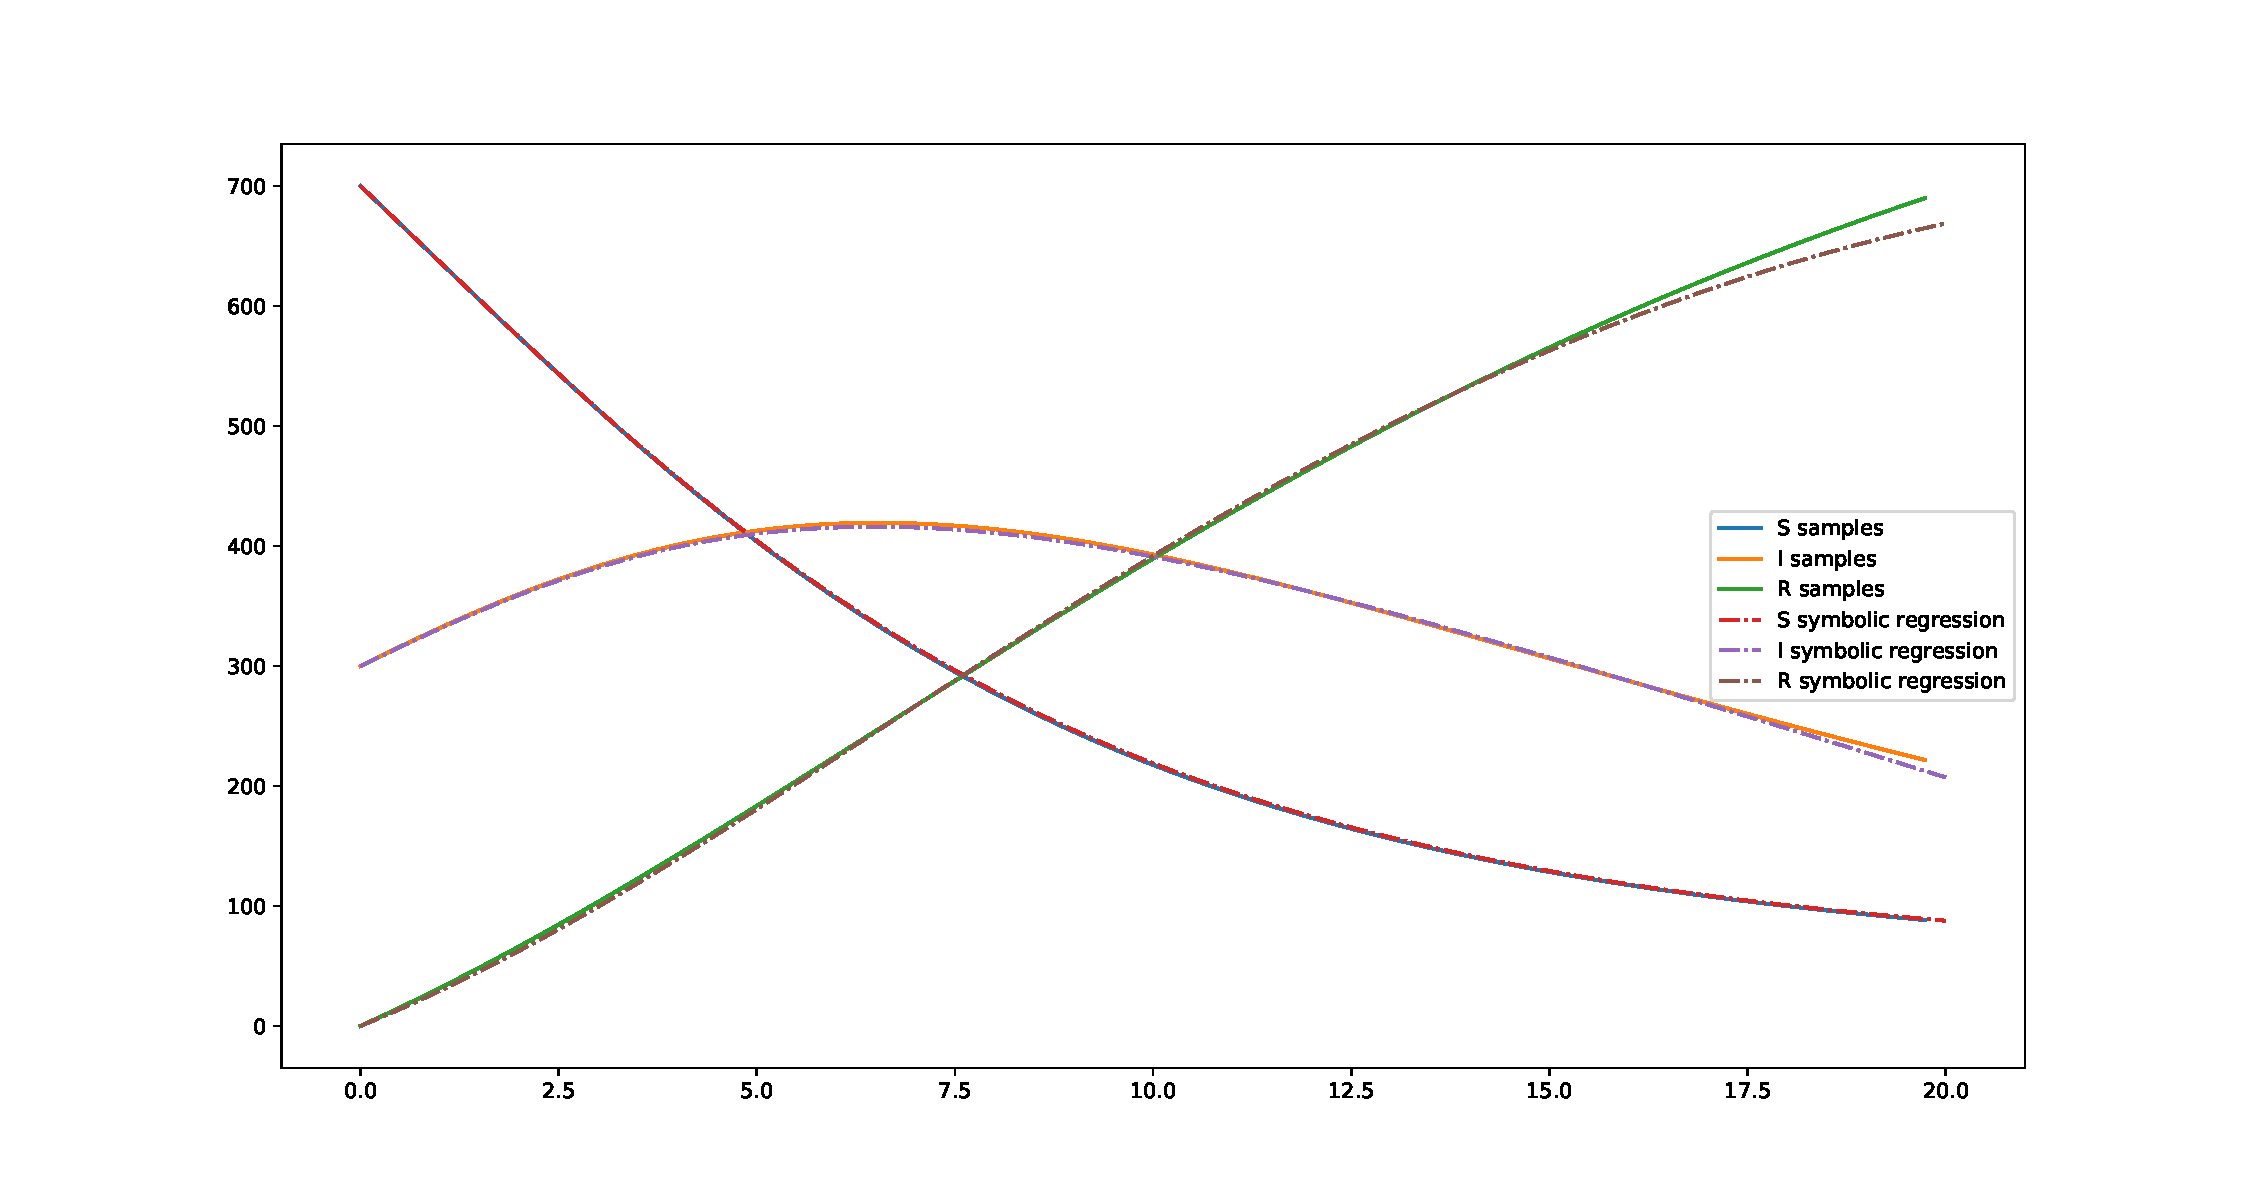
\includegraphics[width=\textwidth]{"figures/final_plot_SIR_0.1.pdf"}
    \begin{align*}
        S' & =  0.02128 * (-(S) / I) + -1.01147 * (((S * I) * I) * I)      \\
        I' & = -0.09552 * I + 0.11332 * (S / I) + -0.02671 * ((S / I) / I) \\
        R' & = -0.09905 * -(I)
    \end{align*}
    \caption{Modelo resultante utilizando datos generados a partir del modelo SIR con ruido máximo de 10\%.}
    \label{fig:final_plot_SIR_0.1}
\end{figure}

Si en lugar de utilizar como aproximación de la derivada el método de diferencias finitas cuando los datos no poseen ruido, se utiliza el sistema original de SIR, se obtiene que la media del valor de la función de ajuste a lo largo de las 30 ejecuciones del experimento es $1.16426e-07$. El valor máximo de la función de ajuste alcanzado fue de $1.16426e-06$ y el mínimo de $1.11311e-18$, en este último la regresión simbólica obtuvo exactamente el sistema utilizado para generar los datos.

A continuación se muestra el experimento realizado a partir de la generación de datos utilizando el sistema SIRD.

\subsection{SIRD}

El modelo SIRD es un sistema similar al SIR pero que introduce como dato la cantidad de personas fallecidas $D$ \cite{bailey1975mathematical}. Al modelo SIRD mencionado en \cite{bailey1975mathematical} se le realizó una modificación al añadir un parámetro representando la cantidad de personas que pasan a ser susceptibles en cada instante de tiempo. El sistema se define como:

\begin{align*}
    S' & = a - b (\frac{S I}{S + I + R})         \\
    I' & = b (\frac{S I}{S + I + R}) - c I - d I \\
    R' & = c I                                   \\
    D' & = d I,
\end{align*}

donde $a$ representa la cantidad de personas que pasan a ser susceptibles, $b$ es el índice de contagio de la enfermedad, $c$ es el índice de recuperación y $d$ es el índice de muerte a causa de la enfermedad.

Se utilizaron como valores de los parámetros $a = 250$, $b = 0.5$, $c = 0.1$ y $d = 0.2$ con punto inicial $(7000, 3000, 0, 0)$ y se integró en el intervalo $0 \leq t \leq 20$ para obtener los datos que aparecen en la figura \ref{fig:SIRD}. Del conjunto de puntos se seleccionaron 300 muestras como datos para el método de regresión simbólica.

\begin{figure}[h]
    \centering
    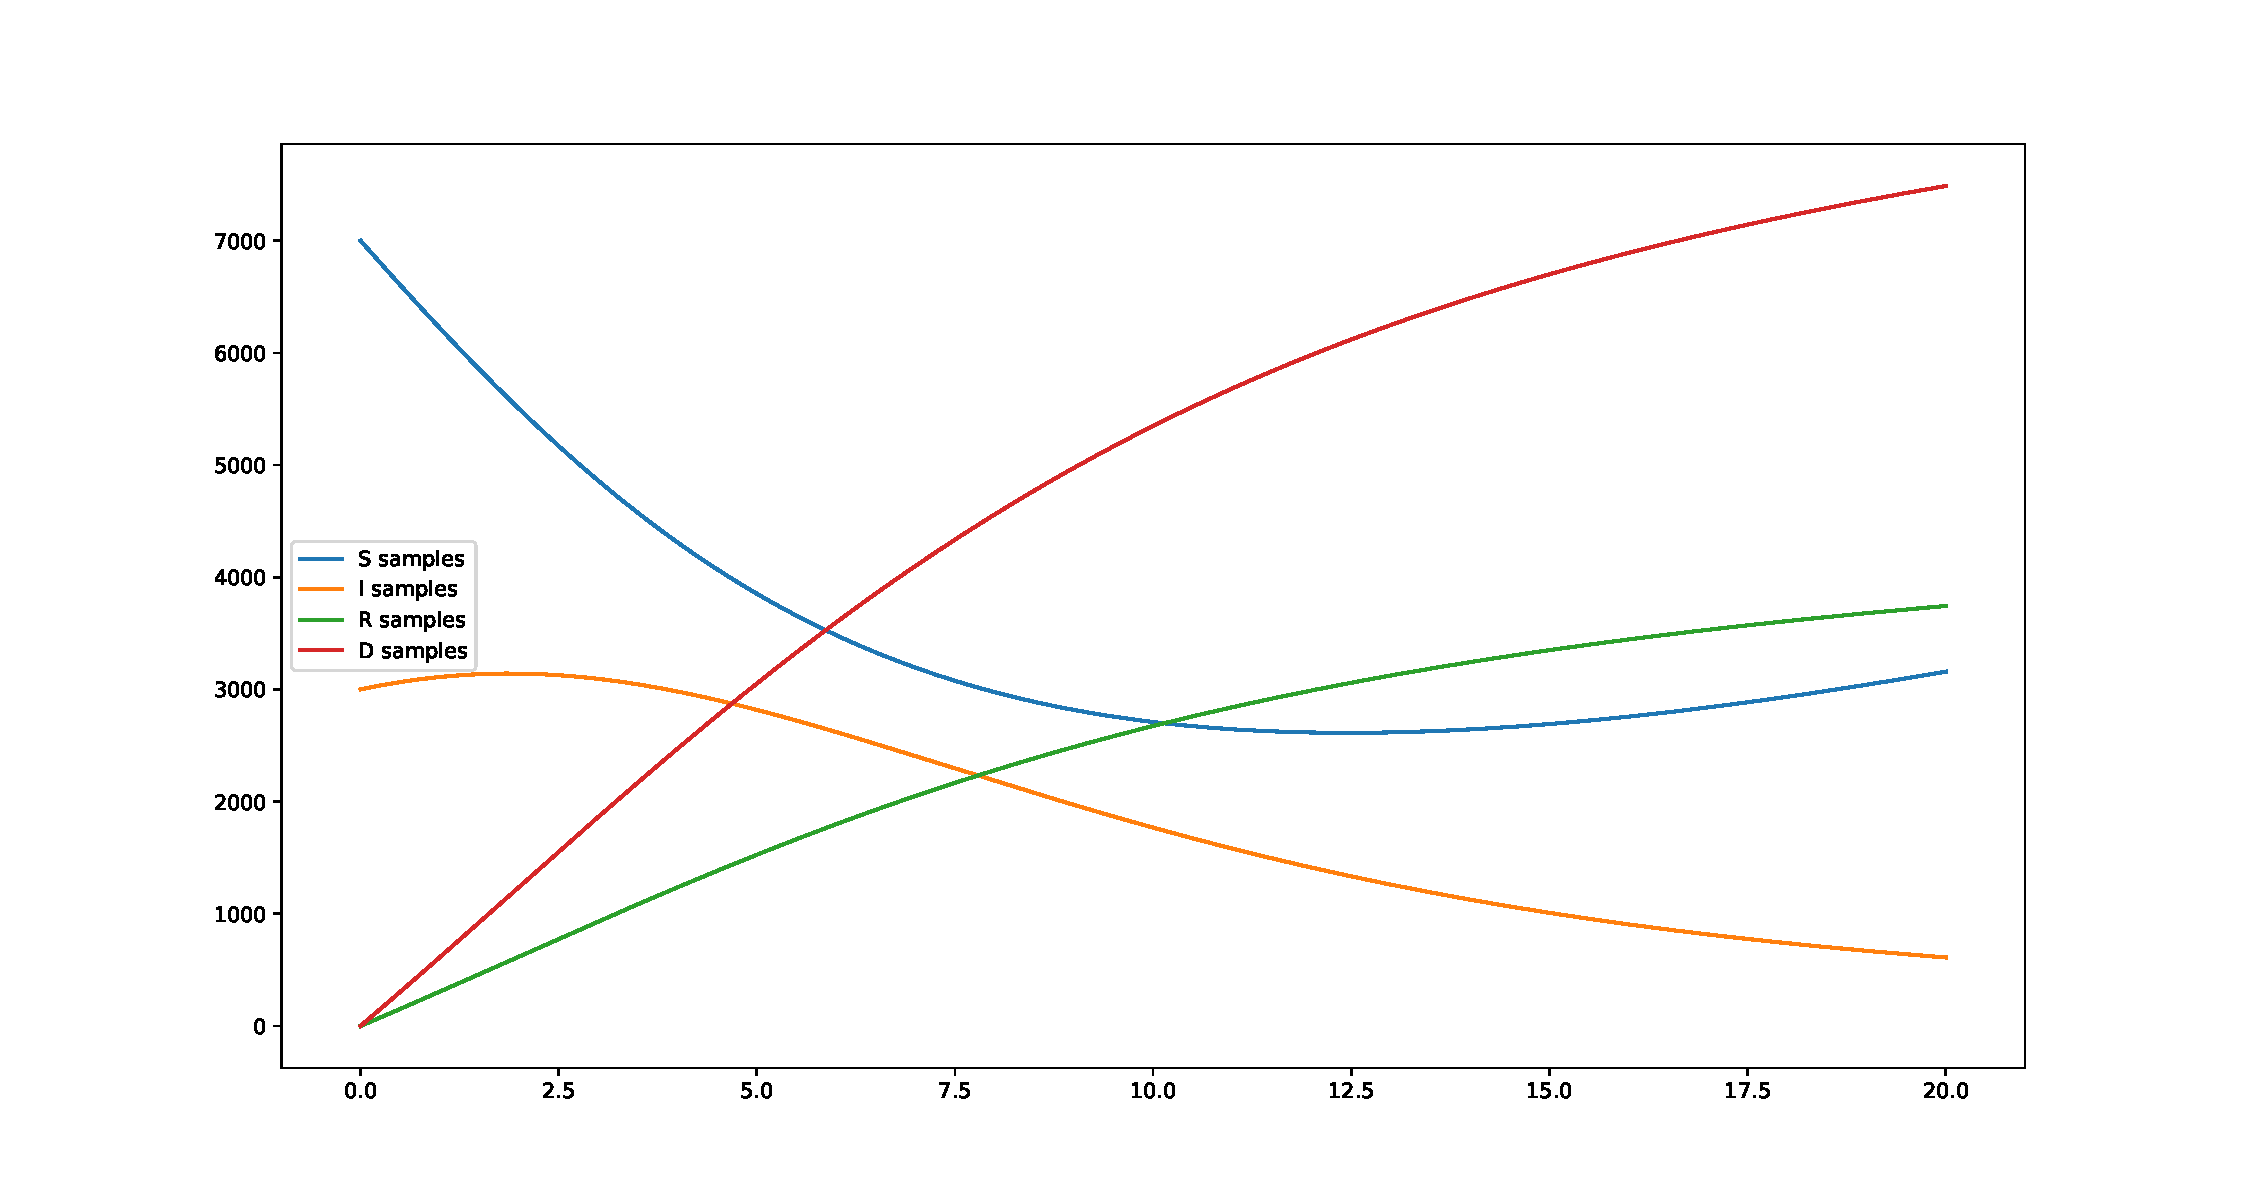
\includegraphics[width=\textwidth]{"figures/SIRD.pdf"}
    \caption{modelo SIRD con $a = 250$, $b = 0.5$, $c = 0.1$ y $d = 0.2$.}
    \label{fig:SIRD}
\end{figure}

Los resultados que se obtienen durante las 30 ejecuciones del experimento, utilizando solamente en cada ecuación las variables permitidas según el modelo y además se agrega como varible $N=S + I + R$, aparecen en la tabla \ref{table:experiment_SIRD} de la página \pageref{table:experiment_SIRD}. Si se permite cualquier variable del modelo en cualquier ecuación del sistema se obtienen los datos que aparecen en la tabla \ref{table:experiment_SIRD_all} de la página \pageref{table:experiment_SIRD_all}.

\begin{table}[!h]
    \centering
    \caption{Resultados que se obtienen en el modelo SIRD restringiendo las variables que aparecen en cada ecuación.}
    \begin{tabular}{|c|c|c|c|}
        \hline
               & \textbf{ruido de 0\%} & \textbf{ruido de 5\%} & \textbf{ruido de 10\%} \\
        \hline
        media  & 47.66074              & 90.64233              & 244.82477              \\
        \hline
        mínimo & 0.51207               & 10.05468              & 18.63161               \\
        \hline
        máximo & 133.55556             & 569.35212             & 2450.05618             \\
        \hline
    \end{tabular}

    \begin{tabular}{|c|c|c|c|c|c|}
        \hline
                             & \textbf{ruido de 0\%} & \textbf{ruido de 5\%} & \textbf{ruido de 10\%} \\
        \hline
        cantidad de sistemas & 22                    & 19                    & 19                     \\
        \hline
        original             & 520.90815             & 810.02775             & 803.13262              \\
        \hline
        original con ruido   & 520.90815             & 834.93575             & 865.07082              \\
        \hline
        spline               & 520.90815             & 810.65156             & 799.79948              \\
        \hline
    \end{tabular}
    \label{table:experiment_SIRD}
\end{table}

\begin{table}[!h]
    \centering
    \caption{Resultados que se obtienen en el modelo SIRD sin restringir las variables que aparecen en cada ecuación.}
    \begin{tabular}{|c|c|c|c|}
        \hline
               & \textbf{ruido de 0\%} & \textbf{ruido de 5\%} & \textbf{ruido de 10\%} \\
        \hline
        media  & 18.06453              & 109.07249             & 40.10858               \\
        \hline
        mínimo & 0.86131               & 10.14889              & 13.82246               \\
        \hline
        máximo & 49.33228              & 2116.3281             & 193.21428              \\
        \hline
    \end{tabular}

    \begin{tabular}{|c|c|c|c|c|c|}
        \hline
                             & \textbf{ruido de 0\%} & \textbf{ruido de 5\%} & \textbf{ruido de 10\%} \\
        \hline
        cantidad de sistemas & 27                    & 23                    & 20                     \\
        \hline
        original             & 248.31329             & 382.03283             & 411.43553              \\
        \hline
        original con ruido   & 248.31329             & 422.02173             & 518.35021              \\
        \hline
        spline               & 248.31329             & 381.52789             & 404.87889              \\
        \hline
    \end{tabular}
    \label{table:experiment_SIRD_all}
\end{table}

Durante la realización de los experimentos utilizando el modelo SIRD nunca se obtuvo un sistema igual como resultado de la regresión simbólica, además la media del error cuadrático medio entre los datos generados por el sistema resultante de la regresión simbólica y los datos utilizados para hallar el sistema es mayor que 15 no importa la cantidad de ruido. El sistema SIRD que se utiliza es el único sistema entre todos los experimentos que posee un término en una ecuación donde aparece un parámetro sin una expresión que lo acompañe, además presenta divisiones con expresiones de más de un término en el divisor.

En las figuras \ref{fig:final_plot_SIRD_0.0} de la página \pageref{fig:final_plot_SIRD_0.0}, \ref{fig:final_plot_SIRD_0.05} de la página \pageref{fig:final_plot_SIRD_0.05} y \ref{fig:final_plot_SIRD_0.1} de la página \pageref{fig:final_plot_SIRD_0.1} se pueden ver los datos originales comparados con los datos obtenidos del mejor resultado generado por la regresión simbólica restringiendo las variables que pueden existir en cada ecuación. Se pueden comparar las figuras \ref{fig:final_plot_SIRD_0.0} y \ref{fig:final_plot_SIRD_0.05} para ver como los datos se asemejan más a los datos originales cuando no existe presencia de ruido.

Los datos que se obtienen de la integración del sistema resultante de la regresión simbólica no se asemejan a los datos de la integración del sistema seleccionado para la realización del experimento, la aparición de ruido afecta aún más el ajuste de los datos.

\begin{figure}[h]
    \centering
    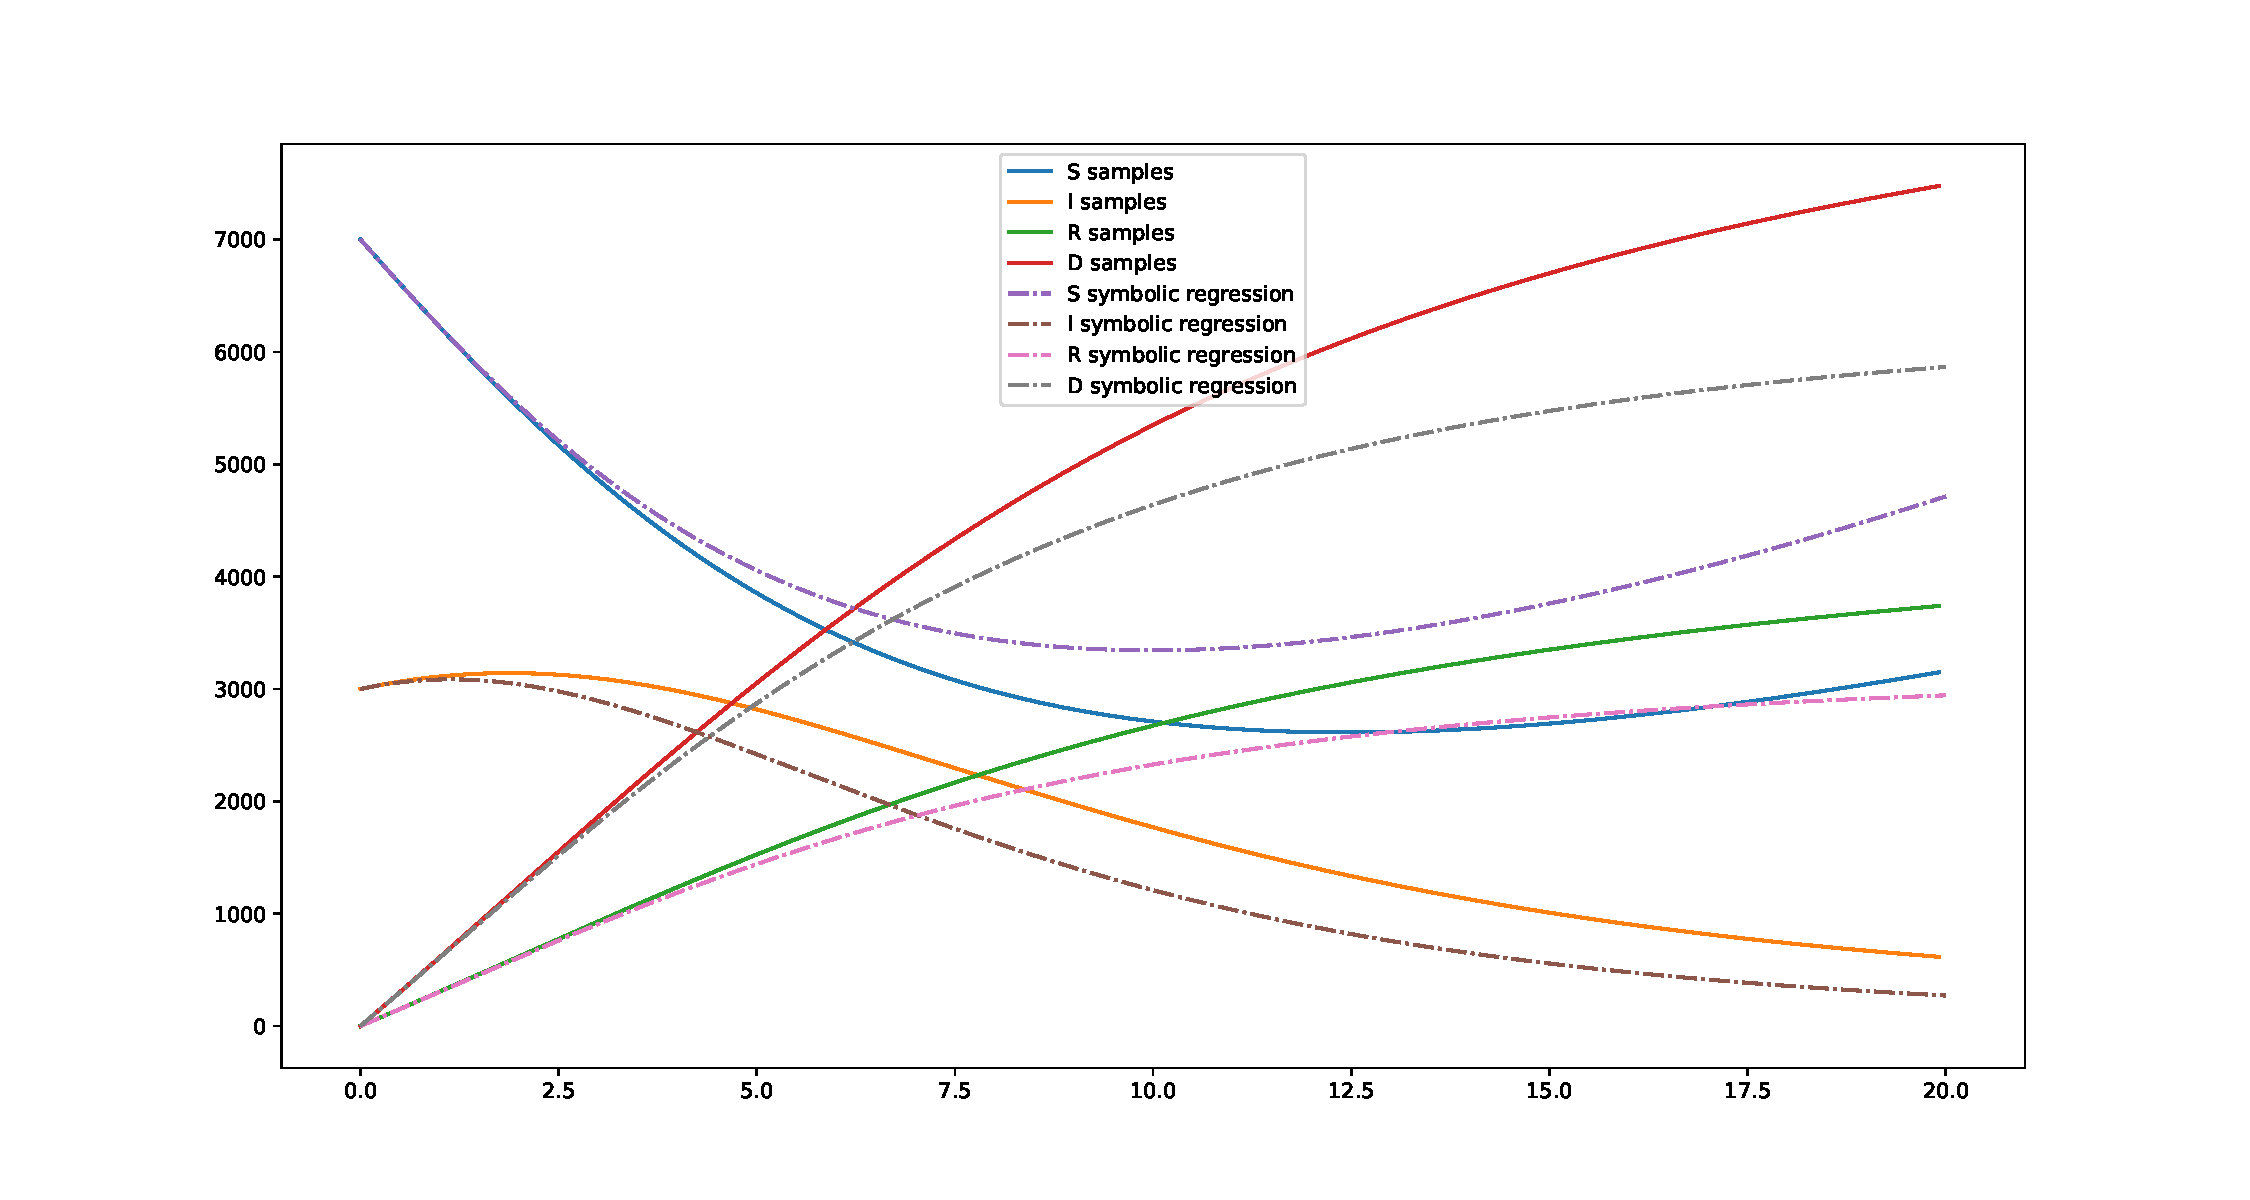
\includegraphics[width=\textwidth]{"figures/final_plot_SIRD_0.0.pdf"}
    \begin{align*}
        S' = & -1159334 * (I - N) + 1159334 * (I + (I / (((S - I) * I) + (N * I)))) \\
             & -1159334 * N -0.01676 * -S                                           \\
        I' = & -0.49543 * -((I * (S / N))) -0.29644 * I -0.00046 * N                \\
             & + 0.00094 * S                                                        \\
        R' = & -0.09983 * -I                                                        \\
        D' = & -0.19898 * -I
    \end{align*}
    \caption{Modelo resultante utilizando datos generados a partir del modelo SIRD con ruido máximo de 0\%.}
    \label{fig:final_plot_SIRD_0.0}
\end{figure}

\begin{figure}[h]
    \centering
    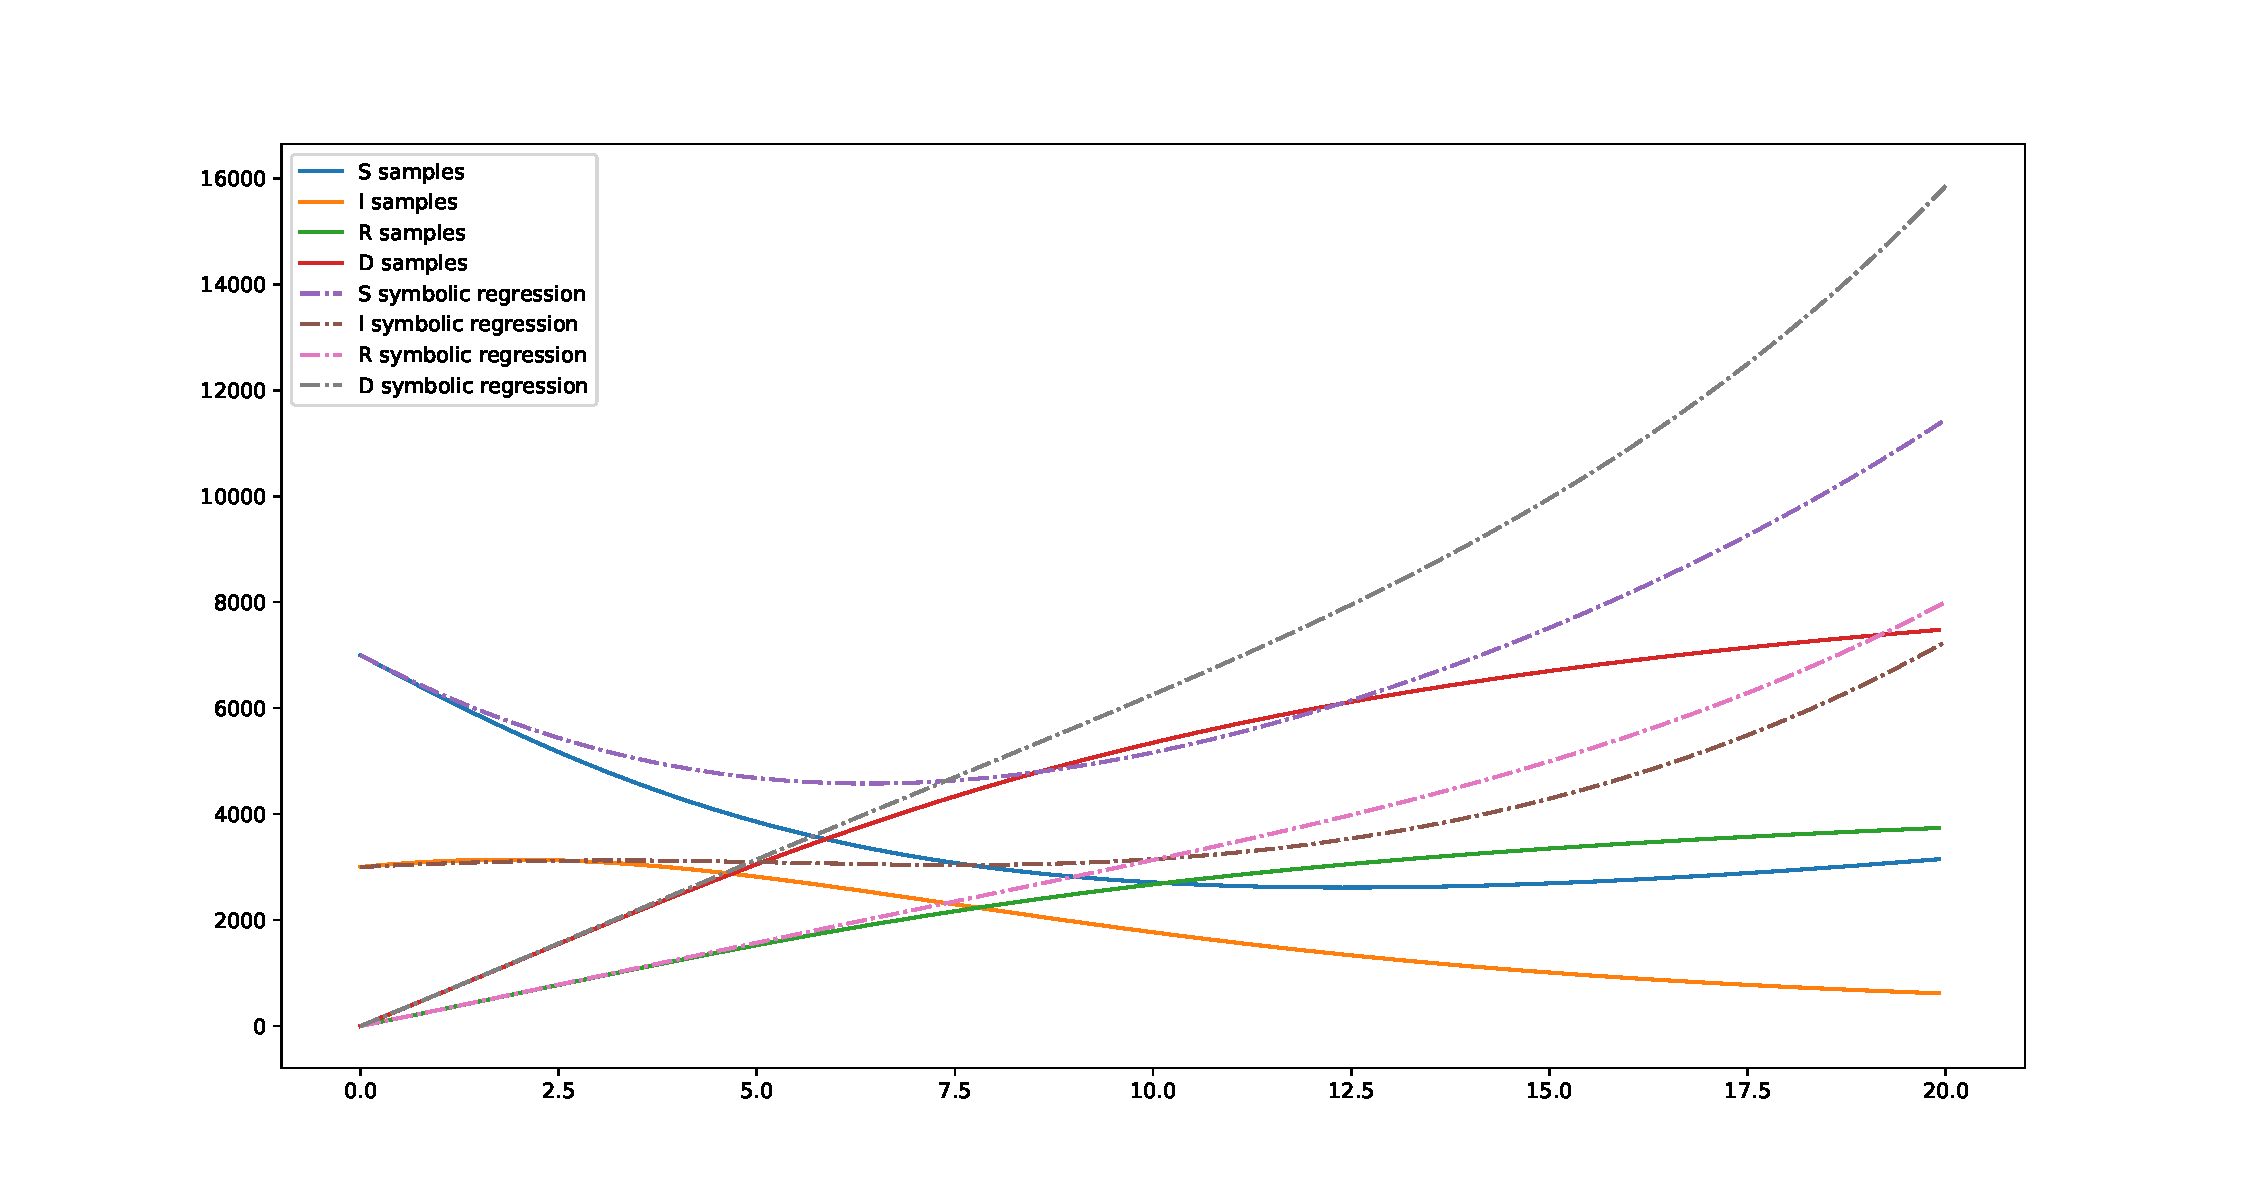
\includegraphics[width=\textwidth]{"figures/final_plot_SIRD_0.05.pdf"}
    \begin{align*}
        S' = & -0.06488 * N -0.22099 * I -0.17175 * (S - N)                                \\
        I' = & 0.03148 * N + 65.45469 * (-(S) / (S - I)) -86.07344 * (N / S)               \\
        R' = & -70.21643 * ((I / (I * I)) * I) + 56352.24282 * (I / (I * I)) + 0.11857 * I \\
        D' = & 0.22264 * I + 48317891.07676 * ((I / I) / (I * I)) -65.24766
    \end{align*}
    \caption{Modelo resultante utilizando datos generados a partir del modelo SIRD con ruido máximo de 5\%.}
    \label{fig:final_plot_SIRD_0.05}
\end{figure}

\begin{figure}[h]
    \centering
    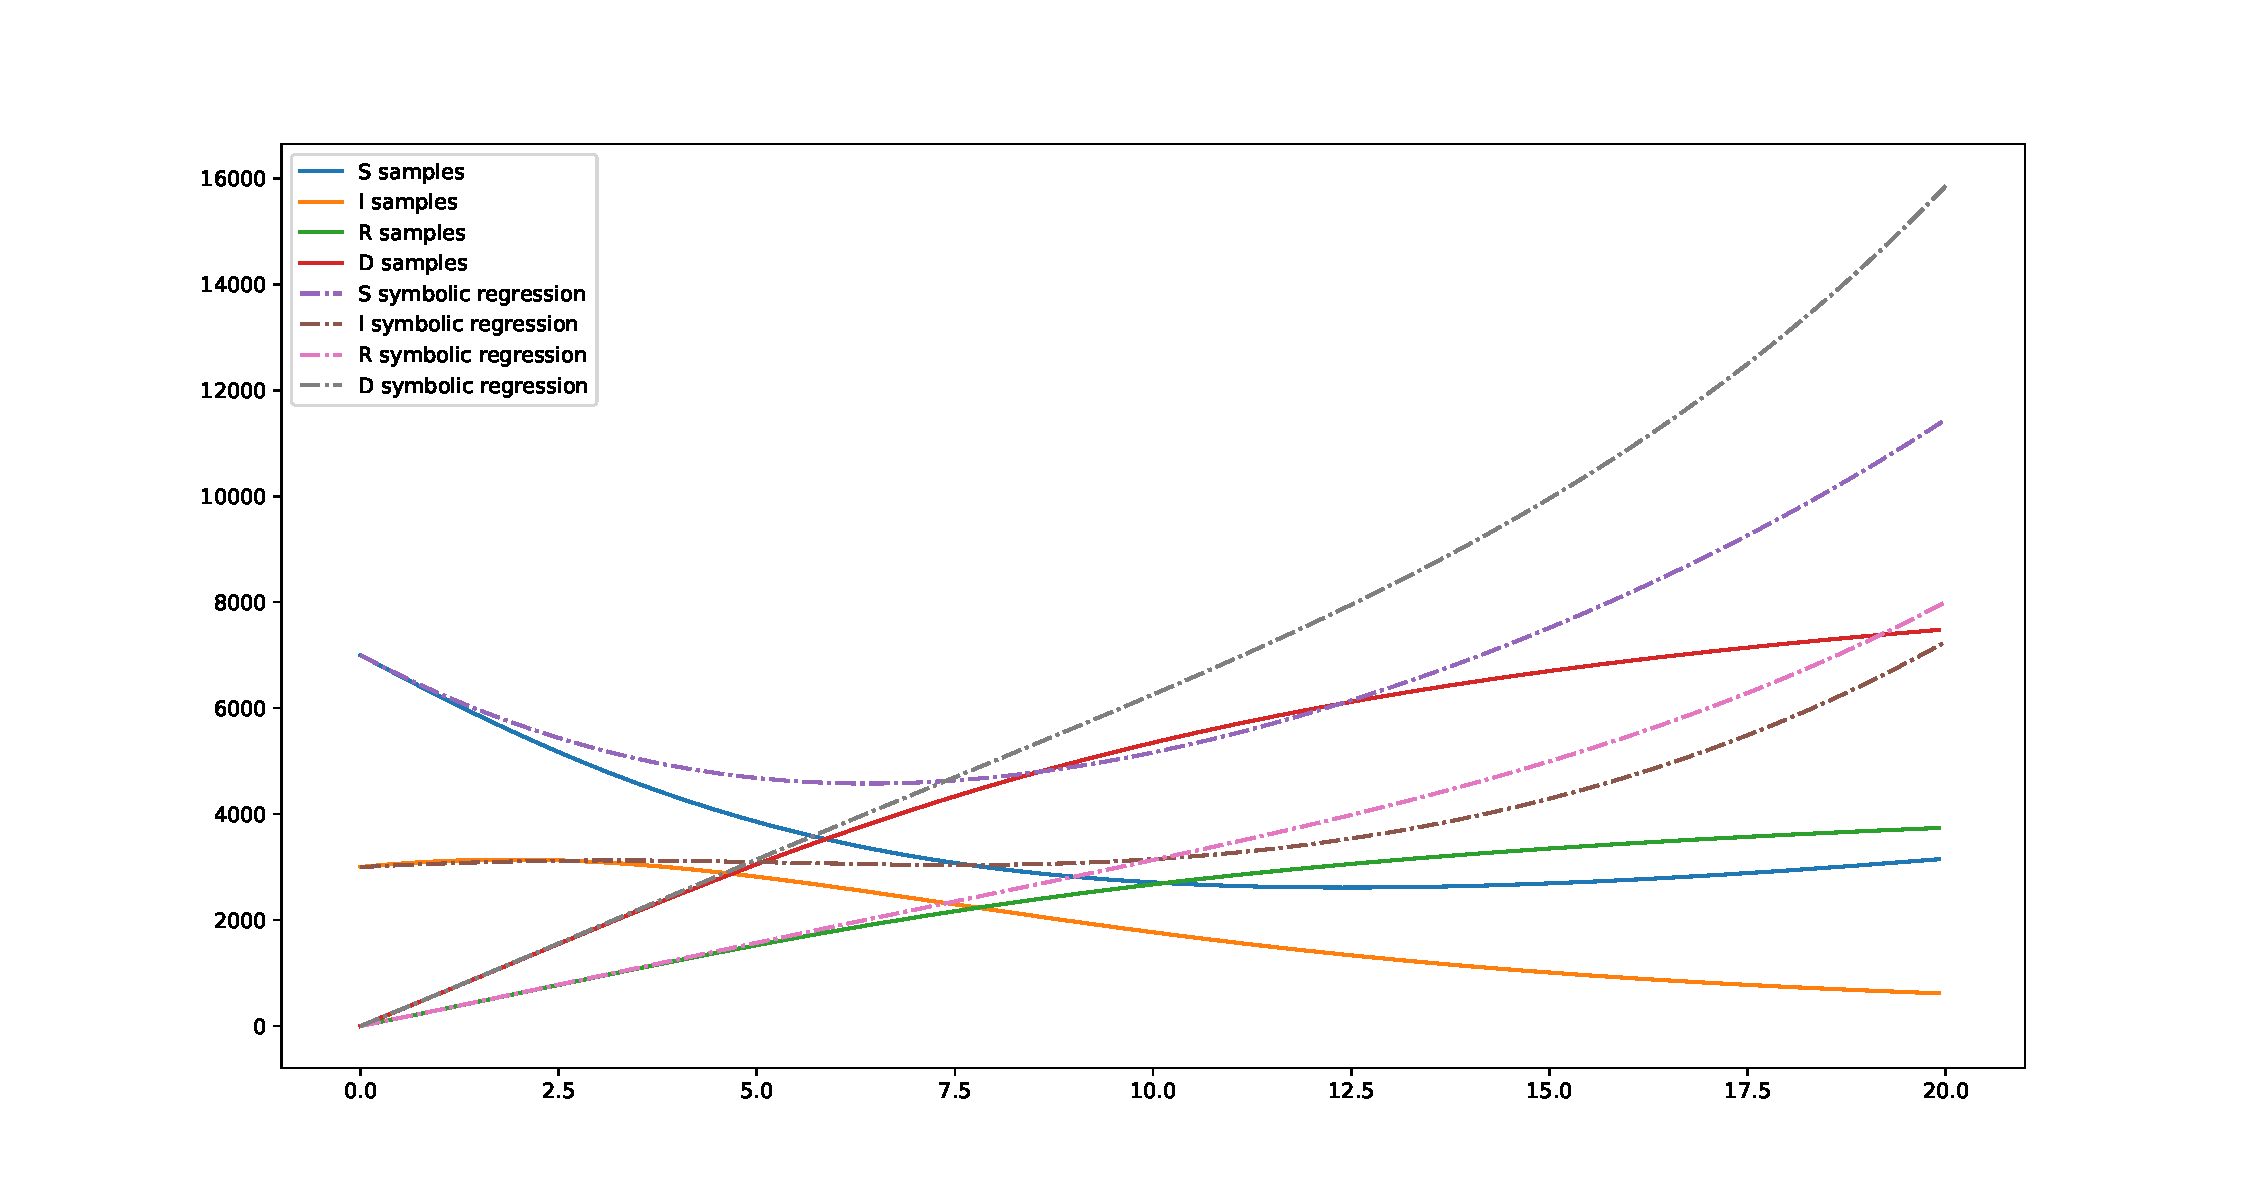
\includegraphics[width=\textwidth]{"figures/final_plot_SIRD_0.1.pdf"}
    \begin{align*}
        S' & = -0.16819 * (N + I) + 1355341.19292 * (N / (N * S)) + 0.1293 * N \\
        I' & = 26.88933 * (N / (I - S)) + 0.03236 * S -82.69305                \\
        R' & = 0.06925 * I -98375.91872 * ((I / I) / I) + 120.68532            \\
        D' & =278798.76253 * ((I - (I + I)) / (I * I)) + 441.12625
    \end{align*}
    \caption{Modelo resultante utilizando datos generados a partir del modelo SIRD con ruido máximo de 10\%.}
    \label{fig:final_plot_SIRD_0.1}
\end{figure}

Si en lugar de utilizar como aproximación el método de diferencias finitas cuando los datos no poseen ruido, se utiliza el sistema original de SIR, se obtiene que la media del valor de la función de ajuste a lo largo de las 30 ejecuciones del experimento es $29.94535$. El valor máximo de la función de ajuste alcanzado fue de $128.83451$ y el mínimo de $2.25834e-14$, en este último la regresión simbólica obtuvo exactamente el sistema utilizado para generar los datos.

A continuación se muestra el experimento realizado a partir de la generación de datos utilizando el sistema SIQRD.

\subsection{SIQRD}

El modelo SIQRD añade al modelo SIRD la posibilidad de aislamiento de una persona, denotado por $Q$, esto modela la situación en que una persona se aisle para no contagiarse o no contagiar a otros \cite{molter2021mathematical}. El sistema se define como:

\begin{align*}
    S' & = -\beta (\frac{S I}{S + I + Q + R + D}) - \alpha S + \delta Q \\
    I' & = \beta (\frac{S I}{S + I + Q + R + D}) - \gamma I - \mu I     \\
    Q' & = \alpha S - \delta Q                                          \\
    R' & = \gamma I                                                     \\
    D' & = \mu I,
\end{align*}

donde $\alpha$ indica la relación con que una persona susceptible es enviada a aislamiento, $\beta$ es el índice de transmisión, $\delta$ indica la relación con que una persona en aislamiento social regresa al grupo de susceptibles, $\gamma$ indica el índice de recuperación y $\mu$ el índice de muerte a causa de la enfermedad.

Se utilizaron como valores de los parámetros $\alpha = 0.2$, $\beta = 0.9$, $\delta = 0.1$, $\gamma = 0.1$ y $\mu = 0.05$ con punto inicial $(5000, 3000, 1000, 0, 0)$ y se integró en el intervalo $0 \leq t \leq 20$ para obtener los datos que aparecen en la imagen \ref{fig:SIQRD} de la página \pageref{fig:SIQRD}. Del conjunto de puntos se seleccionaron 300 muestras como datos para el método de regresión simbólica.

\begin{figure}[h]
    \centering
    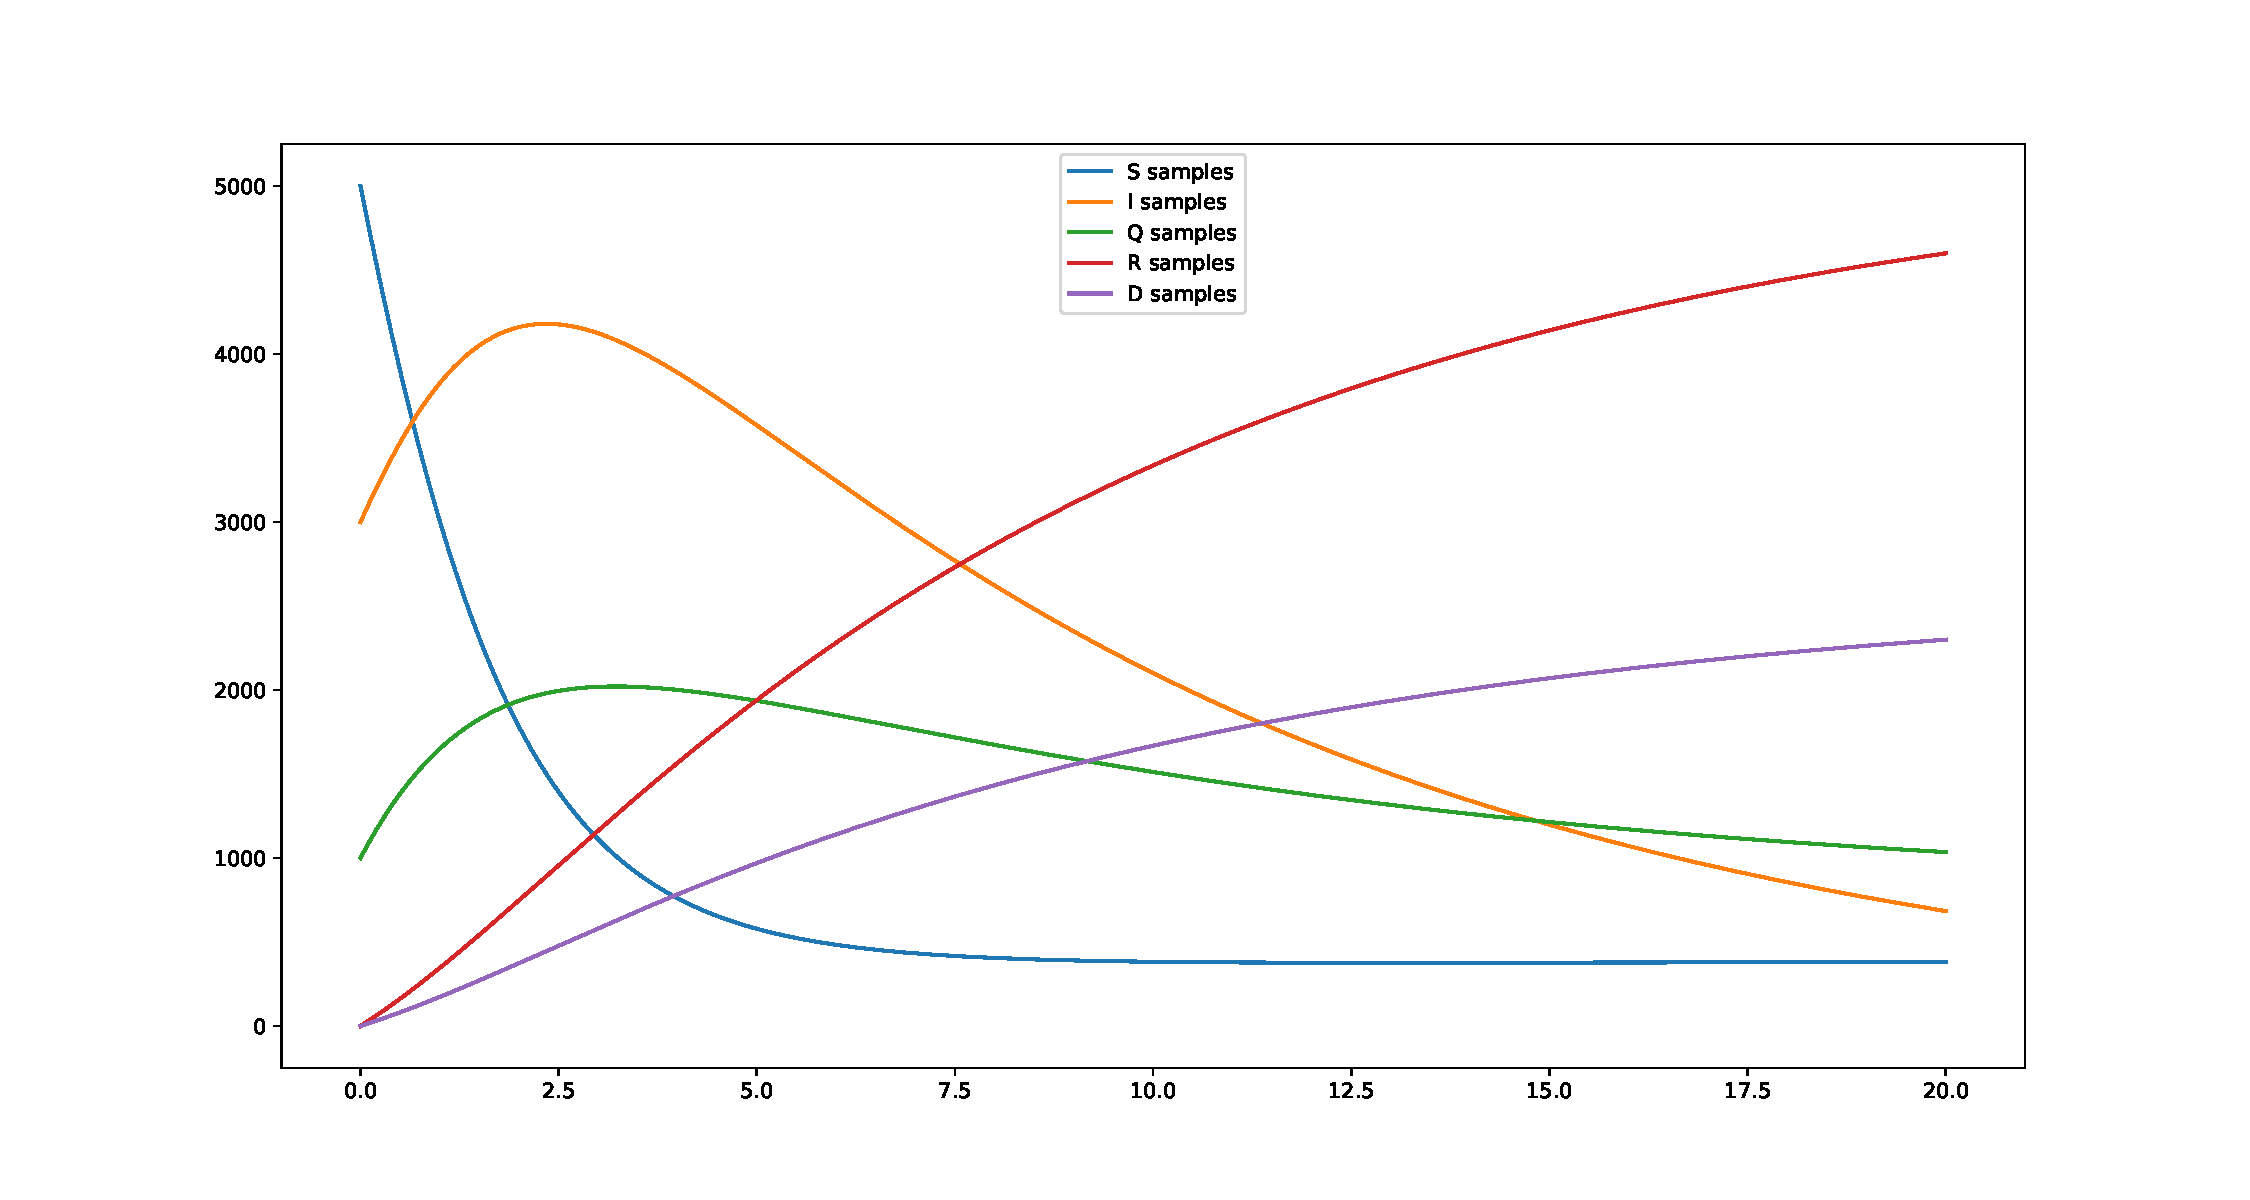
\includegraphics[width=\textwidth]{"figures/SIQRD.pdf"}
    \caption{modelo SIQRD con $\alpha = 0.2$, $\beta = 0.9$, $\delta = 0.1$, $\gamma = 0.1$ y $\mu = 0.05$.}
    \label{fig:SIQRD}
\end{figure}

Los resultados que se obtienen durante las 30 ejecuciones del experimento, utilizando solamente en cada ecuación las variables permitidas según el modelo y además se agrega como varible $N=S + I + Q + R + D$, aparecen en la tabla \ref{table:experiment_SIQRD} de la página \pageref{table:experiment_SIQRD}. Si se permite cualquier variable del modelo en cualquier ecuación del sistema se obtienen los datos que aparecen en la tabla \ref{table:experiment_SIQRD_all} de la página \pageref{table:experiment_SIQRD_all}.

\begin{table}[!h]
    \centering
    \caption{Resultados que se obtienen en el modelo SIQRD restringiendo las variables que aparecen en cada ecuación.}
    \begin{tabular}{|c|c|c|c|}
        \hline
               & \textbf{ruido de 0\%} & \textbf{ruido de 5\%} & \textbf{ruido de 10\%} \\
        \hline
        media  & 7.47098               & 35.17738              & 38.70691               \\
        \hline
        mínimo & 1.35941               & 7.96579               & 12.25428               \\
        \hline
        máximo & 49.24056              & 99.18317              & 197.34403              \\
        \hline
    \end{tabular}

    \begin{tabular}{|c|c|c|c|c|c|}
        \hline
                             & \textbf{ruido de 0\%} & \textbf{ruido de 5\%} & \textbf{ruido de 10\%} \\
        \hline
        cantidad de sistemas & 29                    & 22                    & 22                     \\
        \hline
        original             & 76.49518              & 517.5006              & 338.54534              \\
        \hline
        original con ruido   & 76.49518              & 536.1417              & 395.29378              \\
        \hline
        spline               & 76.49518              & 515.51251             & 338.39969              \\
        \hline
    \end{tabular}
    \label{table:experiment_SIQRD}
\end{table}

\begin{table}[!h]
    \centering
    \caption{Resultados que se obtienen en el modelo SIQRD sin restringir las variables que aparecen en cada ecuación.}
    \begin{tabular}{|c|c|c|c|}
        \hline
               & \textbf{ruido de 0\%} & \textbf{ruido de 5\%} & \textbf{ruido de 10\%} \\
        \hline
        media  & 5.00116               & 34.76361              & 33.05852               \\
        \hline
        mínimo & 2.43638               & 8.78968               & 13.28306               \\
        \hline
        máximo & 7.84816               & 80.32846              & 83.9451                \\
        \hline
    \end{tabular}

    \begin{tabular}{|c|c|c|c|c|c|}
        \hline
                             & \textbf{ruido de 0\%} & \textbf{ruido de 5\%} & \textbf{ruido de 10\%} \\
        \hline
        cantidad de sistemas & 28                    & 19                    & 18                     \\
        \hline
        original             & 55.60273              & 291.27439             & 217.45964              \\
        \hline
        original con ruido   & 55.60273              & 306.48604             & 274.71016              \\
        \hline
        spline               & 55.60273              & 290.19036             & 212.32494              \\
        \hline
    \end{tabular}
    \label{table:experiment_SIQRD_all}
\end{table}

En las figuras \ref{fig:final_plot_SIQRD_0.0} de la página \pageref{fig:final_plot_SIQRD_0.0}, \ref{fig:final_plot_SIQRD_0.05} de la página \pageref{fig:final_plot_SIQRD_0.05} y \ref{fig:final_plot_SIQRD_0.1} de la página \pageref{fig:final_plot_SIQRD_0.1} se pueden ver los datos originales comparados con los datos obtenidos del mejor resultado generado por la regresión simbólica restringiendo las variables que pueden existir en cada ecuación.

Con este experimento se obtiene que los sistemas generados por la regresión simbólica ajustan los datos mientras estos no posean ruido. Los datos que se obtienen de la integración del sistema resultante de la regresión simbólica se asemejan a los datos de la integración del sistema seleccionado para la realización del experimento pero la aparición de ruido afecta el ajuste de los datos. Los datos que se obtienen de la integración del sistema obtenido a partir de un conjunto de datos con ruido máximo de 5\% obtiene peores resultados que si se utiliza como ruido máximo 10\%. Esto se puede deber a un mal ajuste del parámetro de suavizado utilizado en spline de suavizado.

\begin{figure}[h]
    \centering
    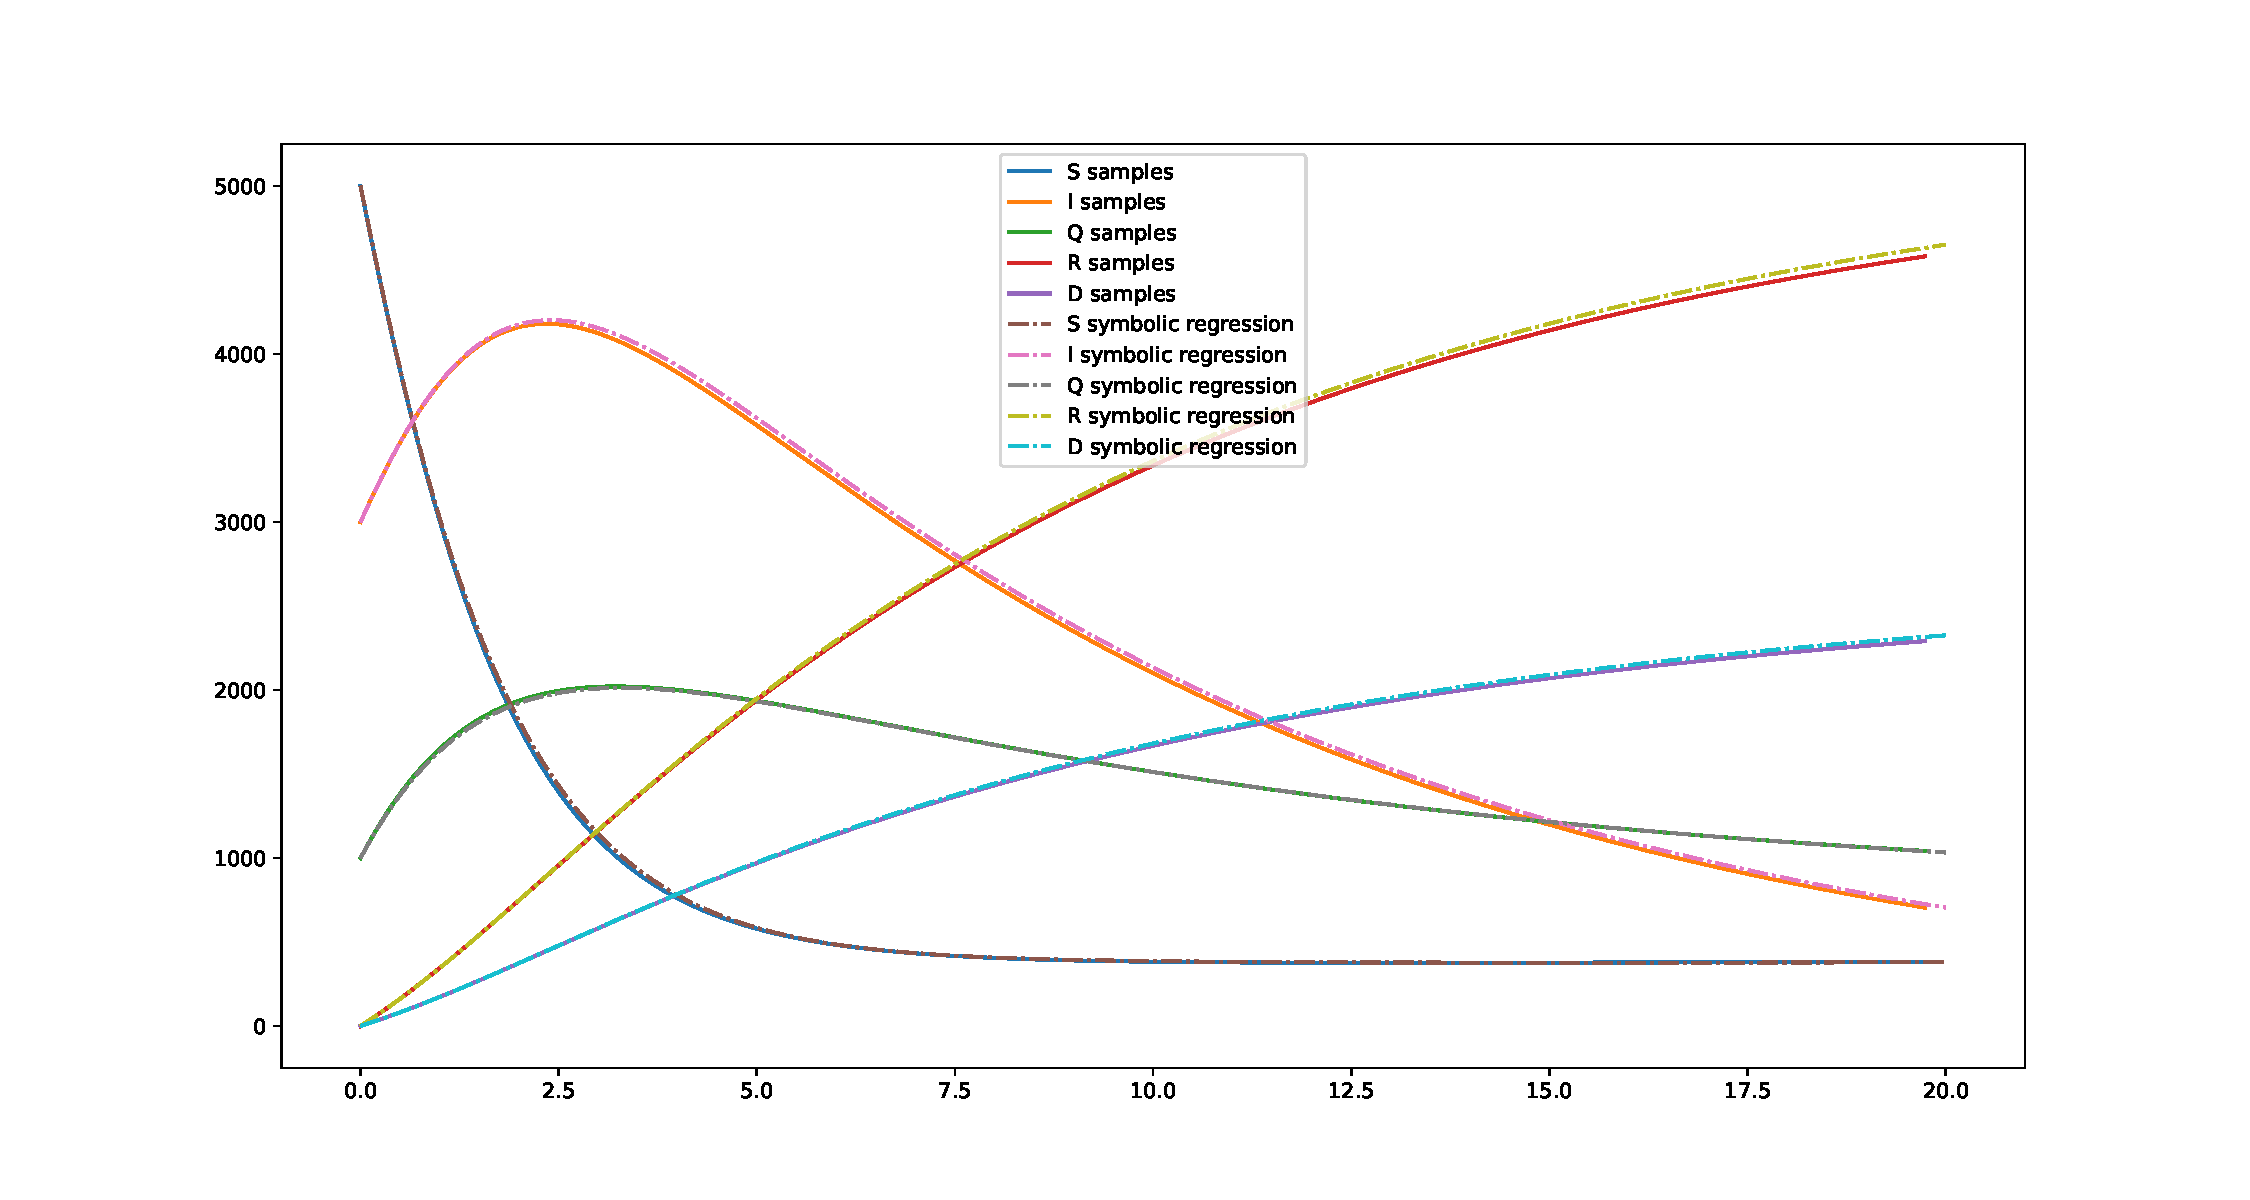
\includegraphics[width=\textwidth]{"figures/final_plot_SIQRD_0.0.pdf"}
    \begin{align*}
        S' = & -196.78057 * ((-(S) - Q) / Q) -11.70524 * -((Q / S)) \\
             & -0.69603 * S -0.00527 * N + 0.01191 * Q              \\
        I' = & 0.0001 * (S * I) -0.14995 * I + 0.06145 * (N / S)    \\
        Q' = & 0.19565 * S -0.09886 * Q                             \\
        R' = & -0.09989 * -I                                        \\
        D' = & 0.04995 * I                                          \\
    \end{align*}
    \caption{Modelo resultante utilizando datos generados a partir del modelo SIQRD con ruido máximo de 0\%.}
    \label{fig:final_plot_SIQRD_0.0}
\end{figure}

\begin{figure}[h]
    \centering
    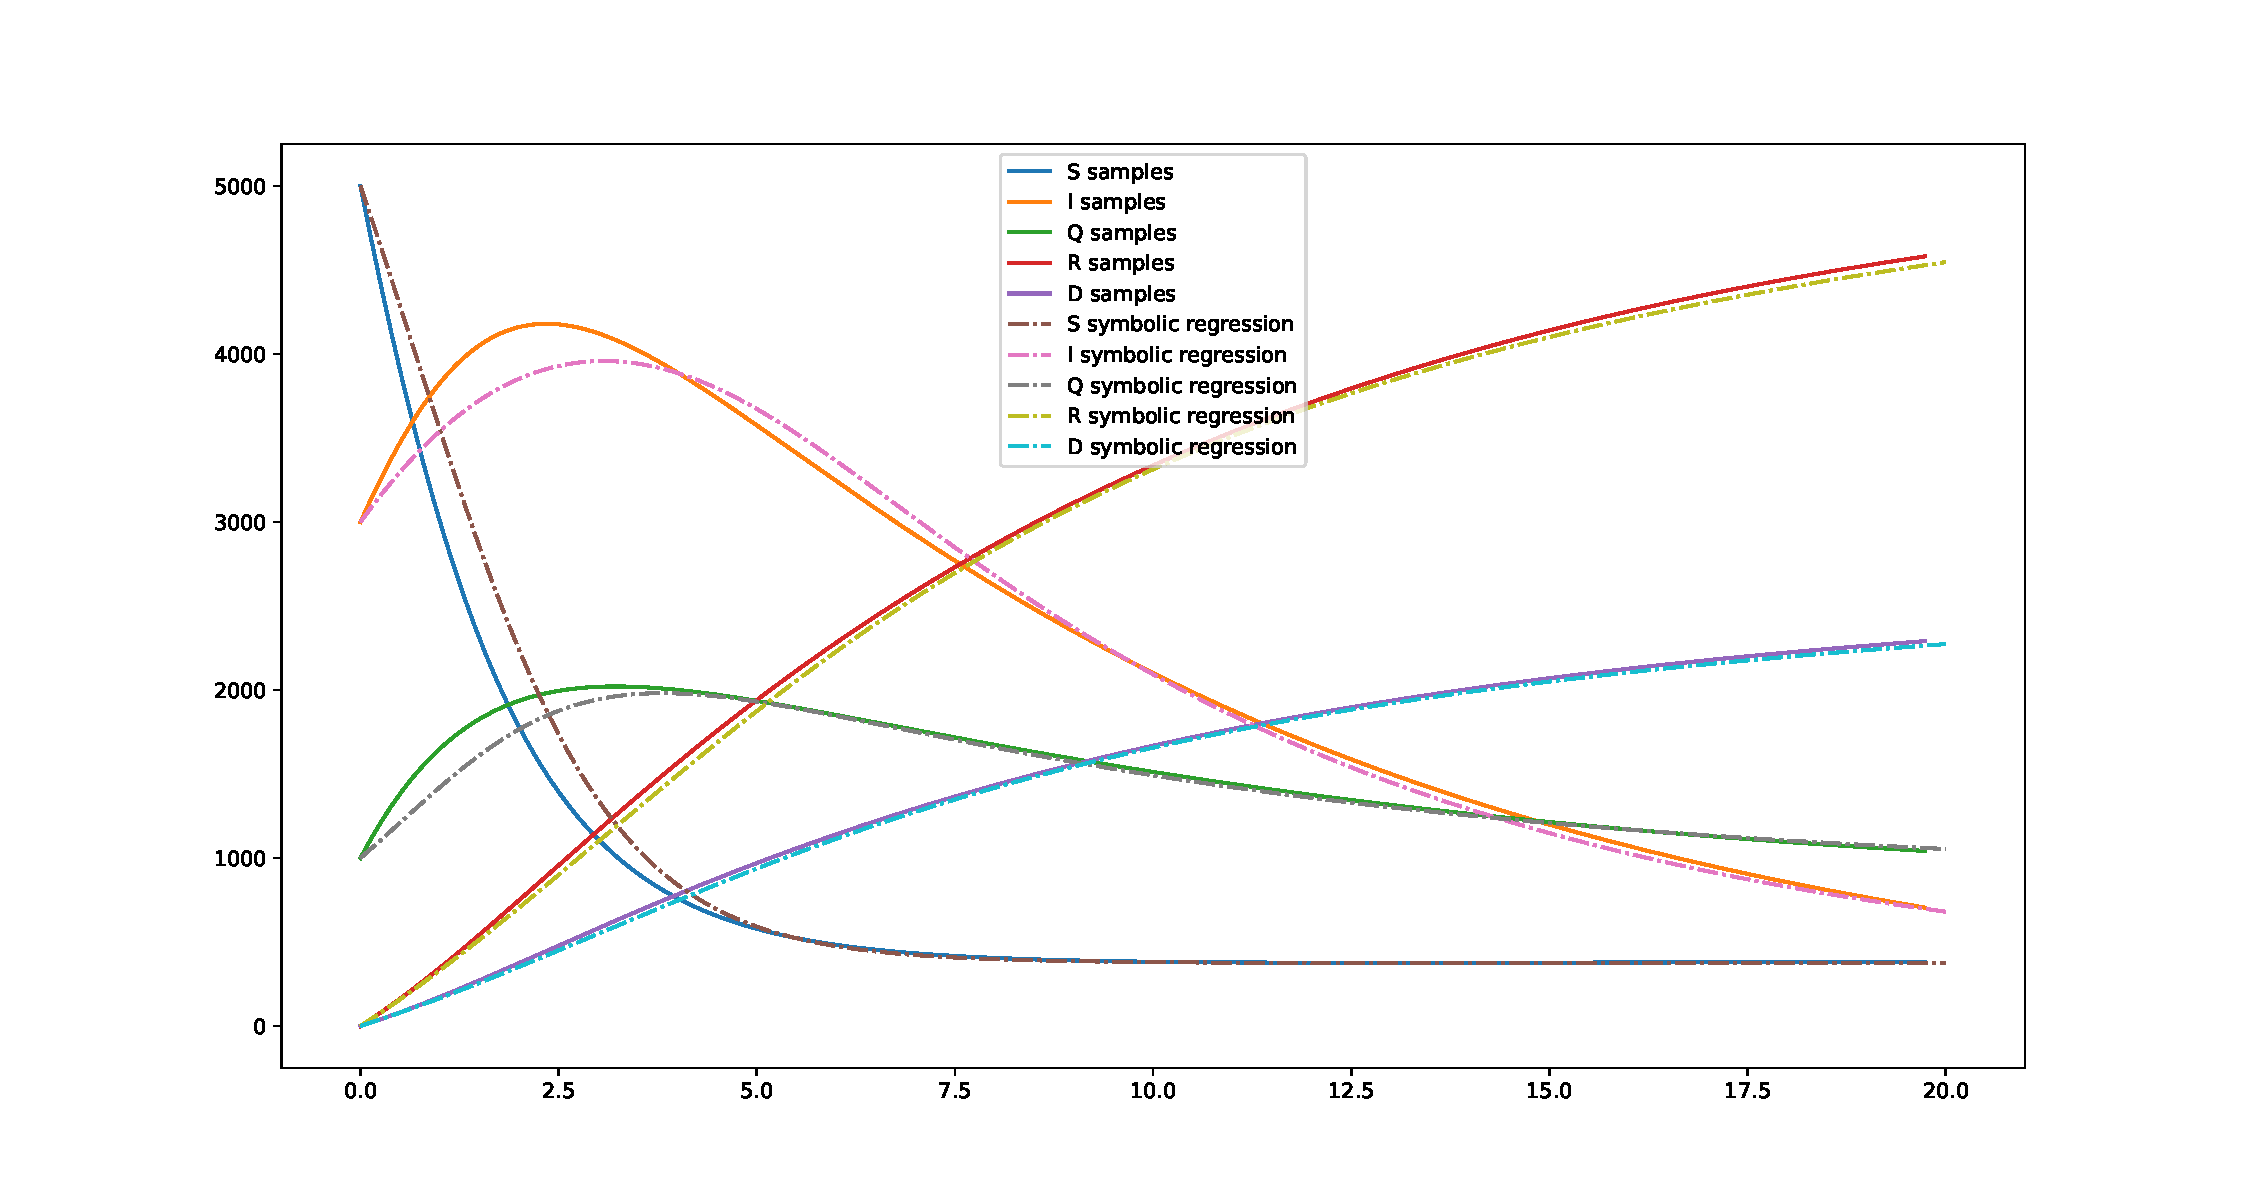
\includegraphics[width=\textwidth]{"figures/final_plot_SIQRD_0.05.pdf"}
    \begin{align*}
        S' = & 0.00011 * (N + (S * S)) + 0.03545 * (N + S) -0.92449 * S     \\
        I' = & 0.00599 * (S - (I * (N / S))) + 0.13448 * S + 0.00215 * -(N) \\
        Q' = & 0.3064 * S -0.1243 * Q                                       \\
        R' = & -0.10052 * -I                                                \\
        D' = & -0.05026 * -I                                                \\
    \end{align*}
    \caption{Modelo resultante utilizando datos generados a partir del modelo SIQRD con ruido máximo de 5\%.}
    \label{fig:final_plot_SIQRD_0.05}
\end{figure}

\begin{figure}[h]
    \centering
    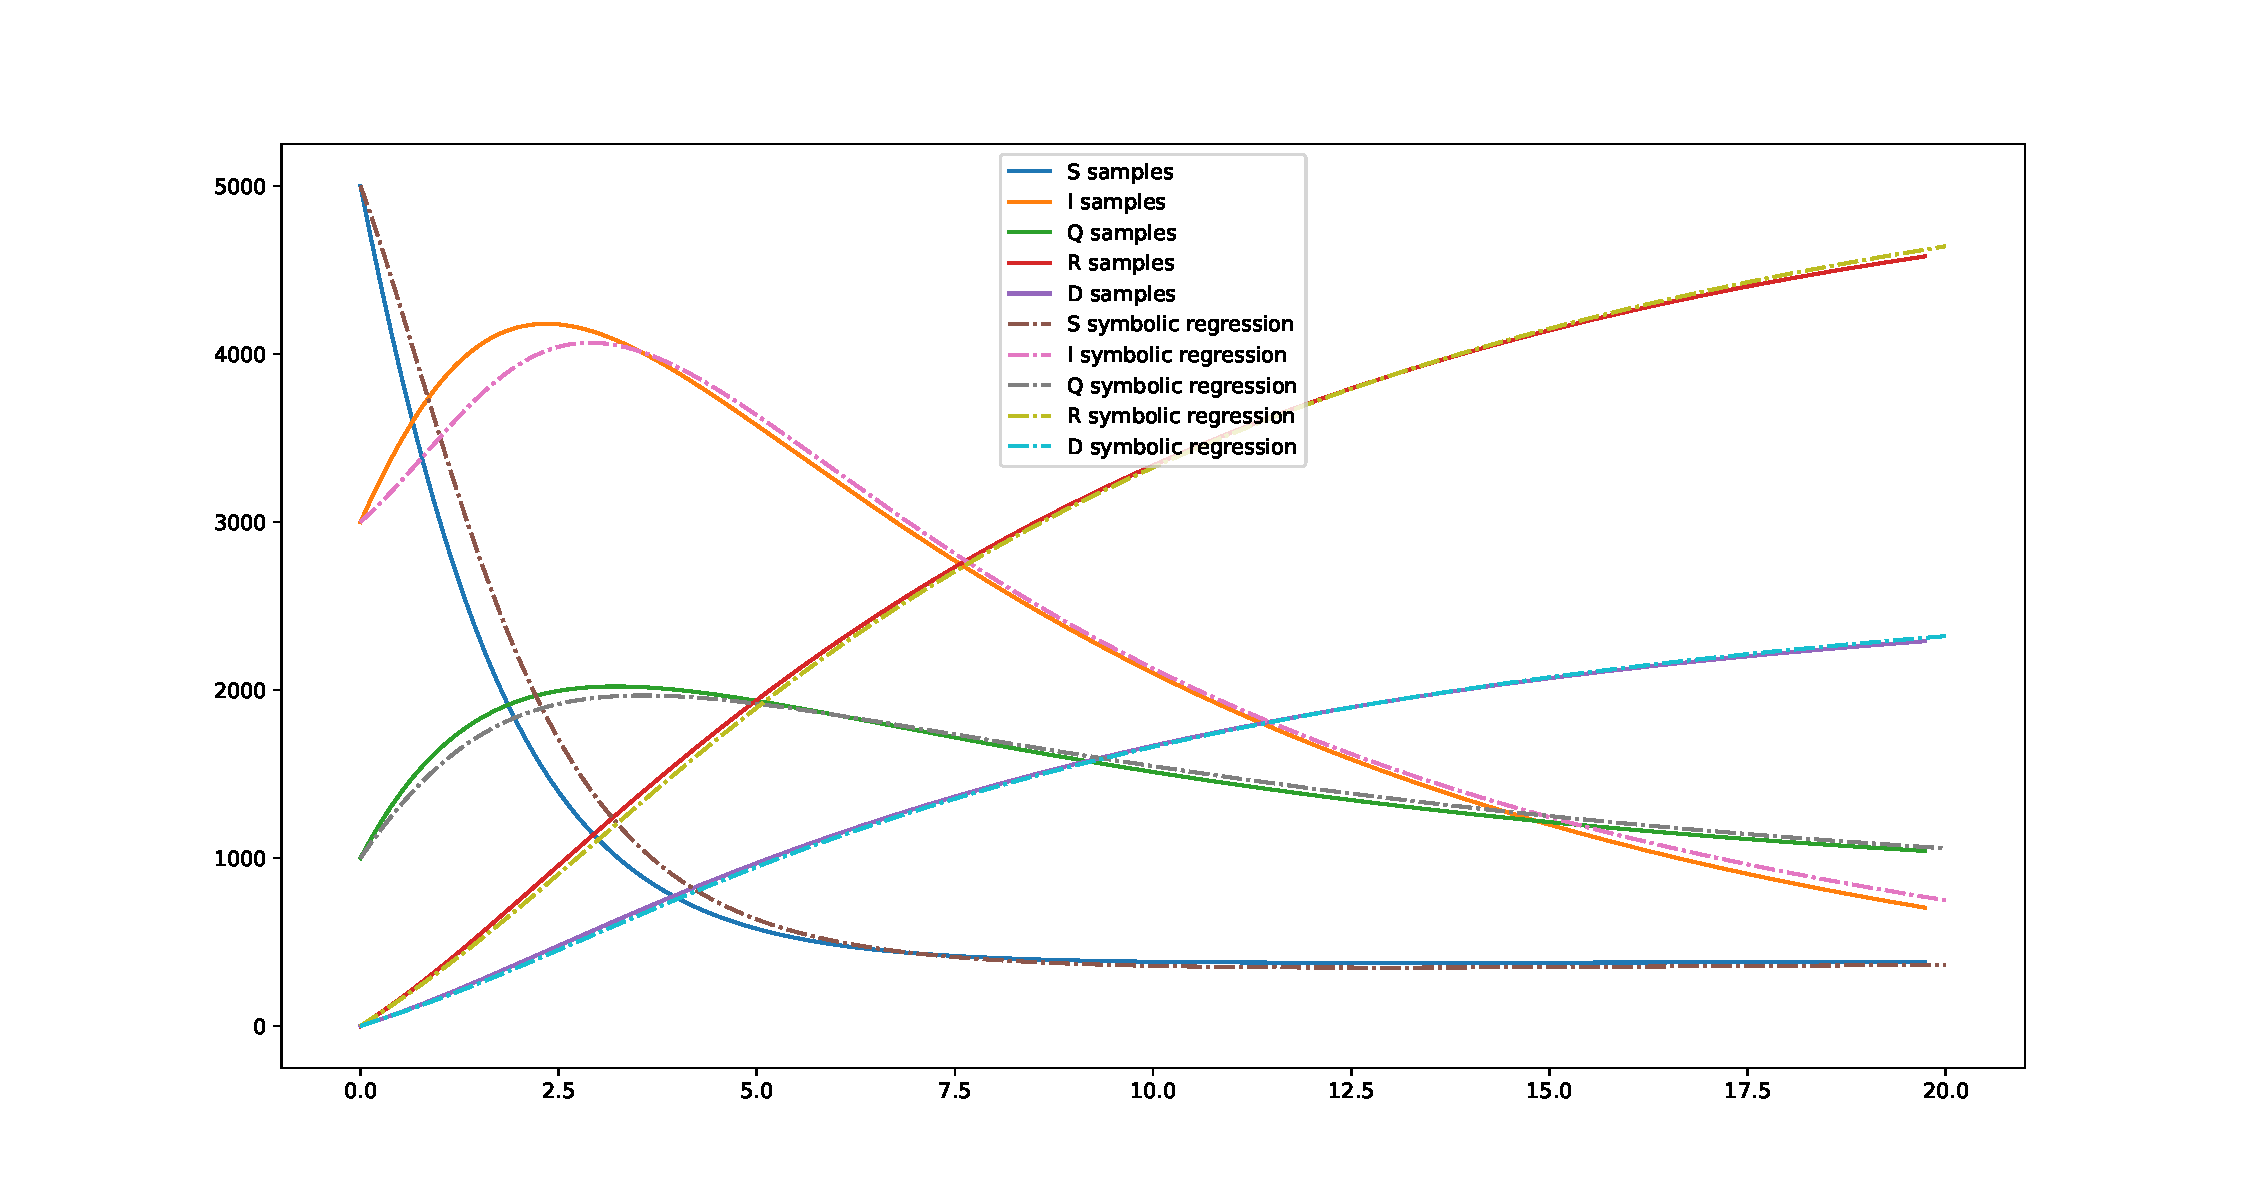
\includegraphics[width=\textwidth]{"figures/final_plot_SIQRD_0.1.pdf"}
    \begin{align*}
        S' = & 0.00035 * -((S * Q)) + -0.01778 * -(N) + 0.14619 * I    \\
             & -0.00012 * (Q * Q)                                      \\
        I' = & 0.00026 * (S * I) -0.02589 * ((I - N) + S) -0.18415 * I \\
             & + 0.59096 * -S                                          \\
        Q' = & -0.08159 * Q + 0.15406 * S                              \\
        R' = & -0.10076 * -I                                           \\
        D' = & 0.05038 * I                                             \\
    \end{align*}
    \caption{Modelo resultante utilizando datos generados a partir del modelo SIQRD con ruido máximo de 10\%.}
    \label{fig:final_plot_SIQRD_0.1}
\end{figure}

Si en lugar de utilizar como aproximación el método de diferencias finitas cuando los datos no poseen ruido, se utiliza el sistema original de SIQRD, se obtiene que la media del valor de la función de ajuste a lo largo de las 30 ejecuciones del experimento es $6.01436$. El valor máximo de la función de ajuste alcanzado fue de $48.48072$ y el mínimo de $1.42392e-14$, en este último la regresión simbólica obtuvo el sistema:

\begin{align*}
    S' & = -0.1 * S -0.1 * S -0.0001 * (I * S) + 0.1 * Q \\
    I' & = -0.075 * I + 0.0001 * (S * I) -0.075 * I      \\
    Q' & = -0.1 * Q + 0.2 * S                            \\
    R' & = -0.1 * -I                                     \\
    D' & = 0.025 * I + 0.025 * I,
\end{align*}

que es igual al sistema original si se asume $\frac{\beta}{N} = 0.0001$.

A continuación se muestra el experimento realizado a partir de la generación de datos utilizando el sistema SVVEIR.

\subsection{SVVEIR}

El modelo SVVEIR describe un escenario de una posible enfermedad en la sociedad de Bangladesh. En el modelo se plantea un conjunto $S$ de individuos que no se han infectado aún, $V_1$ y $V_2$ son los individuos que han recibido la primera y segunda vacuna, respectivamente. Las personas infectadas pero que aún no han desarrollado síntomas se definen como expuestos y se encuentran representados por el conjunto $E$. Los parámetros $I$ y $R$ identifican los mismos conjuntos que en el modelo SIR \cite{kuddus2021mathematical}. El sistema se define como:


\begin{align*}
    N    & = S + V_1 + V_2 + E + I + R                                        \\
    S'   & = \mu * N - \beta * \frac{I}{N} * S - n * S - \mu * S + \rho * V_1 \\
    V_1' & = n * S - \rho * V_1 - \sigma * V_1 - \mu * V_1                    \\
    V_2' & = \sigma * V_1 - \omega * V_2 - \mu * V_2                          \\
    E'   & = \beta * I / N * S - \alpha * E - \mu * E                         \\
    I'   & = \alpha * E - \gamma * I - \delta * I - \mu * I                   \\
    R'   & = \gamma * I + \omega * V_2 - \mu * R,
\end{align*}

donde $\alpha$ indica la relación de personas expuestas que pasan a estar infectados, $\beta$ es el índice de transmisión de la enfermedad, $\delta$ es el índice de muerte debido a la enfermedad mientras que $\mu$ es el índice de muerte por causas naturales. El índice de recuperación de la enfermedad se representa mediante el parámetro $\gamma$. El parámetro $n$ muestra el índice de personas susceptibles que reciben la primera dosis de la vacuna y $\rho$ describe la relación de personas con una sola dosis de la vacuna que regresan al grupo de susceptibles. La cantidad de personas que reciben la segunda dosis se refleja en el parámetro $\sigma$ y $\omega$ es el parámetro que muestra la relación de personas con dos dosis de la vacuna que pasan a recuperados.

Se utilizaron como valores de los parámetros $\alpha = 0.1$, $\beta = 0.7$, $\delta = 0.0005$, $\gamma = 0.05$, $\mu = 0.01$, $n = 0.2$, $\rho = 0.01$, $\omega = 0.05$ y $\sigma = 0.2$ con punto inicial $(5000, 1000, 0, 2000, 1000, 500)$ y se integró en el intervalo $0 \leq t \leq 20$ para obtener los datos que aparecen en la figura \ref{fig:SVVEIR} de la página \pageref{fig:SVVEIR}. Del conjunto de puntos se seleccionaron 300 muestras como datos para el método de regresión simbólica.

\begin{figure}[h]
    \centering
    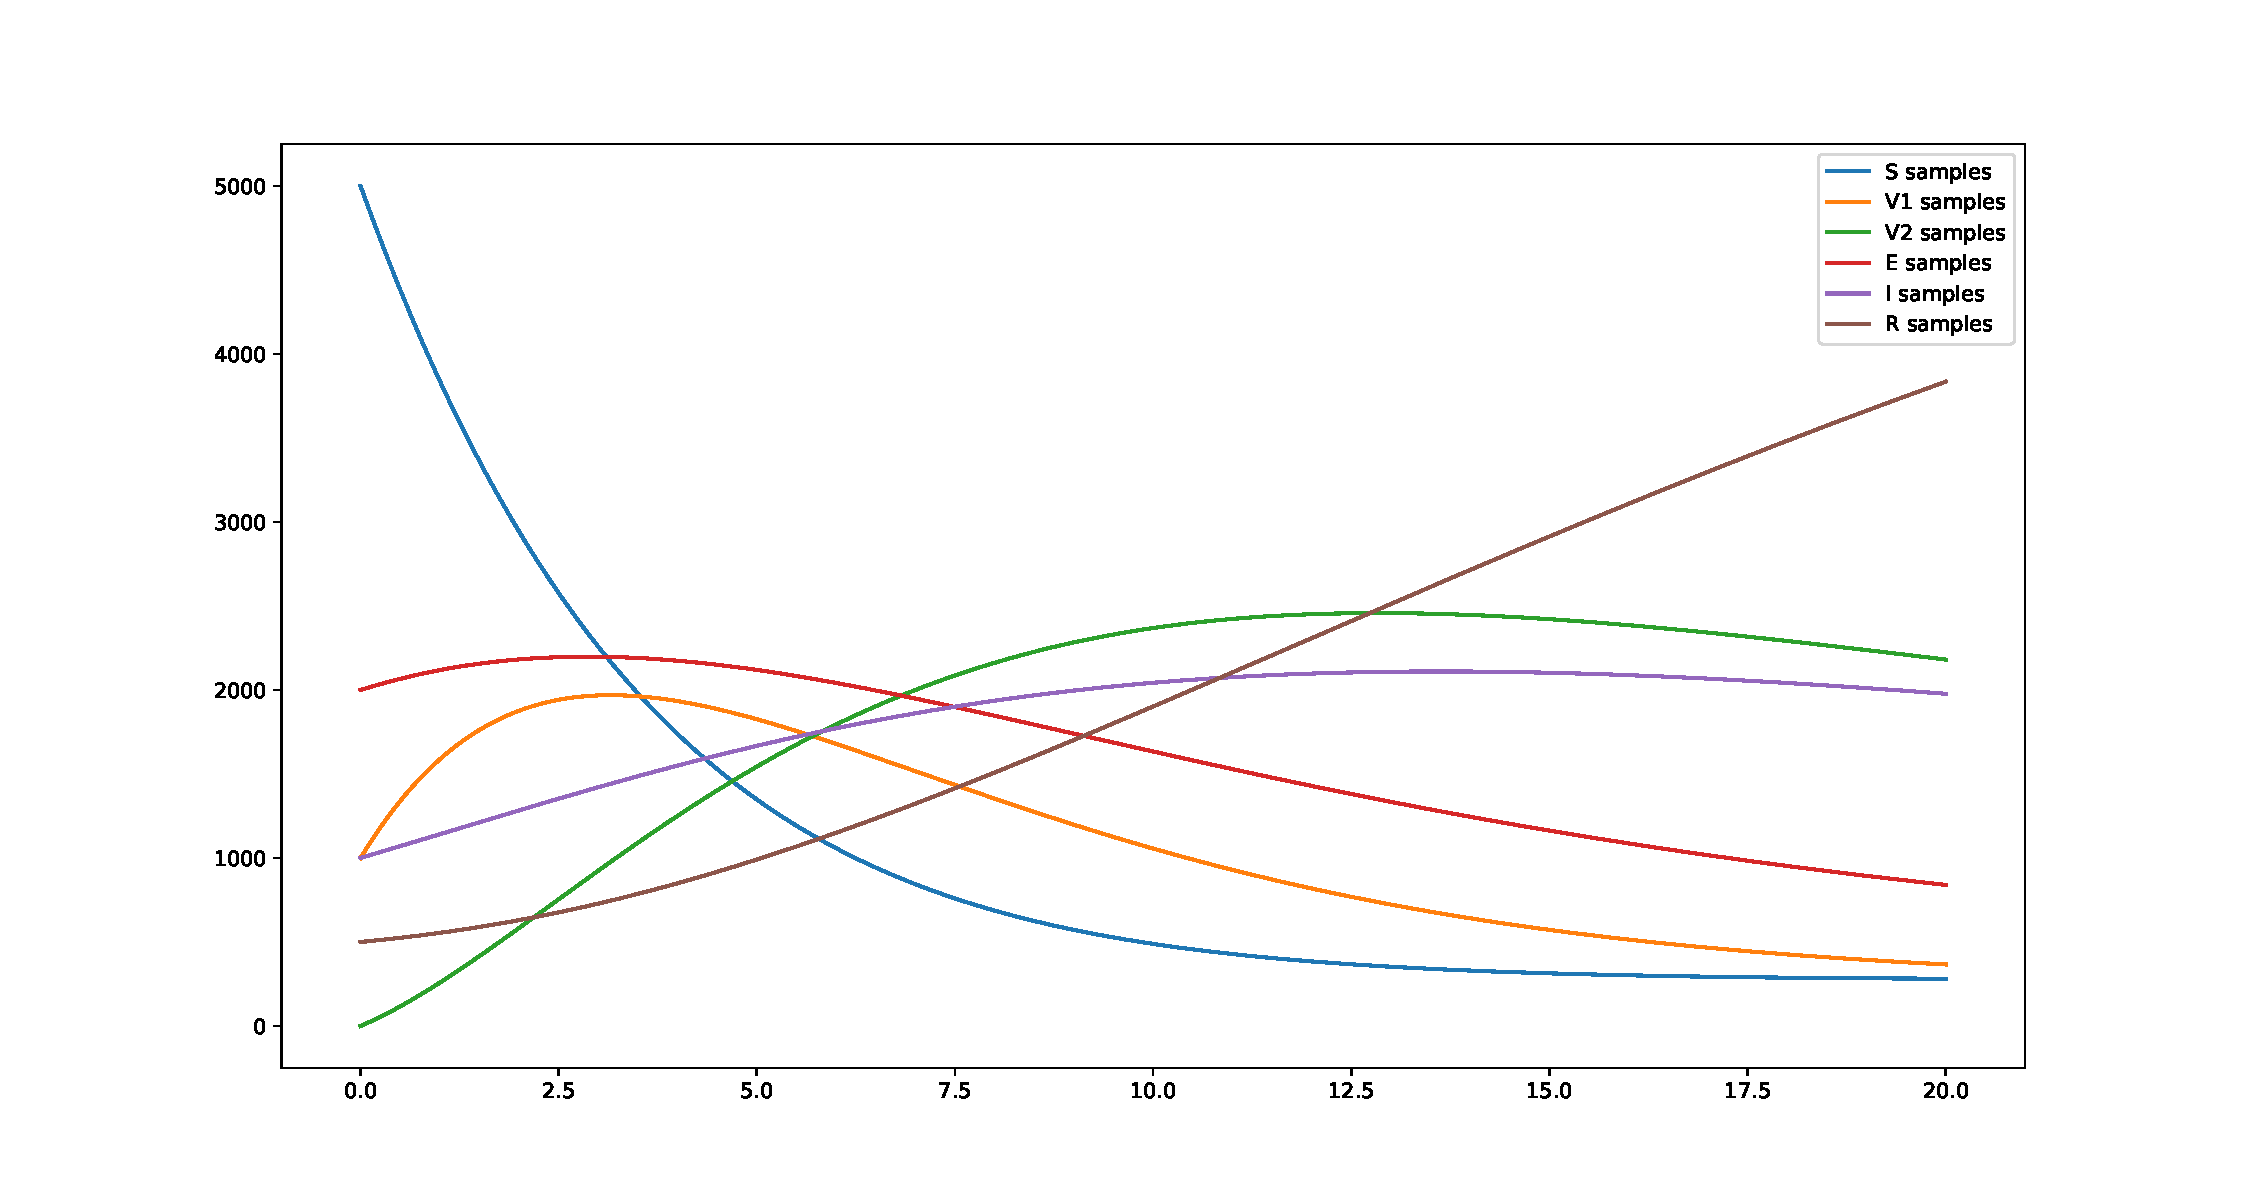
\includegraphics[width=\textwidth]{"figures/SVVEIR.pdf"}
    \caption{modelo SVVEIR con $\alpha = 0.1$, $\beta = 0.7$, $\delta = 0.0005$, $\gamma = 0.05$, $\mu = 0.01$, $n = 0.2$, $\rho = 0.01$, $\omega = 0.05$ y $\sigma = 0.2$.}
    \label{fig:SVVEIR}
\end{figure}

Los resultados que se obtienen durante las 30 ejecuciones del experimento, utilizando solamente en cada ecuación las variables permitidas según el modelo y además se agrega como varible $N=S + V_1 + V_2 + E + I + R$, aparecen en la tabla \ref{table:experiment_SVVEIR} de la página \pageref{table:experiment_SVVEIR}. Si se permite cualquier variable del modelo en cualquier ecuación del sistema se obtienen los datos que aparecen en la tabla \ref{table:experiment_SVVEIR_all} de la página \pageref{table:experiment_SVVEIR_all}. Restringir las variables permitidas en cada ecuación del modelo, y agregar el valor de $N$ como dato disminuyó la media del error cuadrático medio en un valor cercano a $100$.

\begin{table}[!h]
    \centering
    \caption{Resultados que se obtienen en el modelo SVVEIR restringiendo las variables que aparecen en cada ecuación.}
    \begin{tabular}{|c|c|c|c|}
        \hline
               & \textbf{ruido de 0\%} & \textbf{ruido de 5\%} & \textbf{ruido de 10\%} \\
        \hline
        media  & 3.64426               & 13.57802              & 16.12164               \\
        \hline
        mínimo & 1.30096               & 9.50931               & 12.69225               \\
        \hline
        máximo & 14.28797              & 29.02875              & 25.4523                \\
        \hline
    \end{tabular}

    \begin{tabular}{|c|c|c|c|c|c|}
        \hline
                             & \textbf{ruido de 0\%} & \textbf{ruido de 5\%} & \textbf{ruido de 10\%} \\
        \hline
        cantidad de sistemas & 30                    & 30                    & 29                     \\
        \hline
        original             & 26.41261              & 121.61259             & 94.25209               \\
        \hline
        original con ruido   & 26.41261              & 146.93245             & 165.1642               \\
        \hline
        spline               & 26.41261              & 121.72339             & 94.75343               \\
        \hline
    \end{tabular}
    \label{table:experiment_SVVEIR}
\end{table}

\begin{table}[!h]
    \centering
    \caption{Resultados que se obtienen en el modelo SVVEIR sin restringir las variables que aparecen en cada ecuación.}
    \begin{tabular}{|c|c|c|c|}
        \hline
               & \textbf{ruido de 0\%} & \textbf{ruido de 5\%} & \textbf{ruido de 10\%} \\
        \hline
        media  & 8.30945               & 15.87176              & 17.95833               \\
        \hline
        mínimo & 1.76748               & 10.78393              & 12.29942               \\
        \hline
        máximo & 45.85105              & 47.08811              & 44.09112               \\
        \hline
    \end{tabular}

    \begin{tabular}{|c|c|c|c|c|c|}
        \hline
                             & \textbf{ruido de 0\%} & \textbf{ruido de 5\%} & \textbf{ruido de 10\%} \\
        \hline
        cantidad de sistemas & 30                    & 28                    & 30                     \\
        \hline
        original             & 146.5678              & 215.51733             & 173.10665              \\
        \hline
        original con ruido   & 146.5678              & 234.37447             & 230.006                \\
        \hline
        spline               & 146.5678              & 216.31001             & 172.30783              \\
        \hline
    \end{tabular}
    \label{table:experiment_SVVEIR_all}
\end{table}

En las figuras \ref{fig:final_plot_SVVEIR_0.0} de la página \pageref{fig:final_plot_SVVEIR_0.0}, \ref{fig:final_plot_SVVEIR_0.05} de la página \pageref{fig:final_plot_SVVEIR_0.05} y \ref{fig:final_plot_SVVEIR_0.1} de la página \pageref{fig:final_plot_SVVEIR_0.1} se pueden ver los datos originales comparados con los datos obtenidos del mejor resultado generado por la regresión simbólica restringiendo las variables que pueden existir en cada ecuación.

Con este experimento se obtiene que los sistemas generados por la regresión simbólica ajustan los datos mientras estos no posean ruido. Los datos que se obtienen de la integración del sistema resultante de la regresión simbólica se asemejan a los datos de la integración del sistema seleccionado para la realización del experimento pero la aparición de ruido afecta el ajuste de los datos.

\begin{figure}[h]
    \centering
    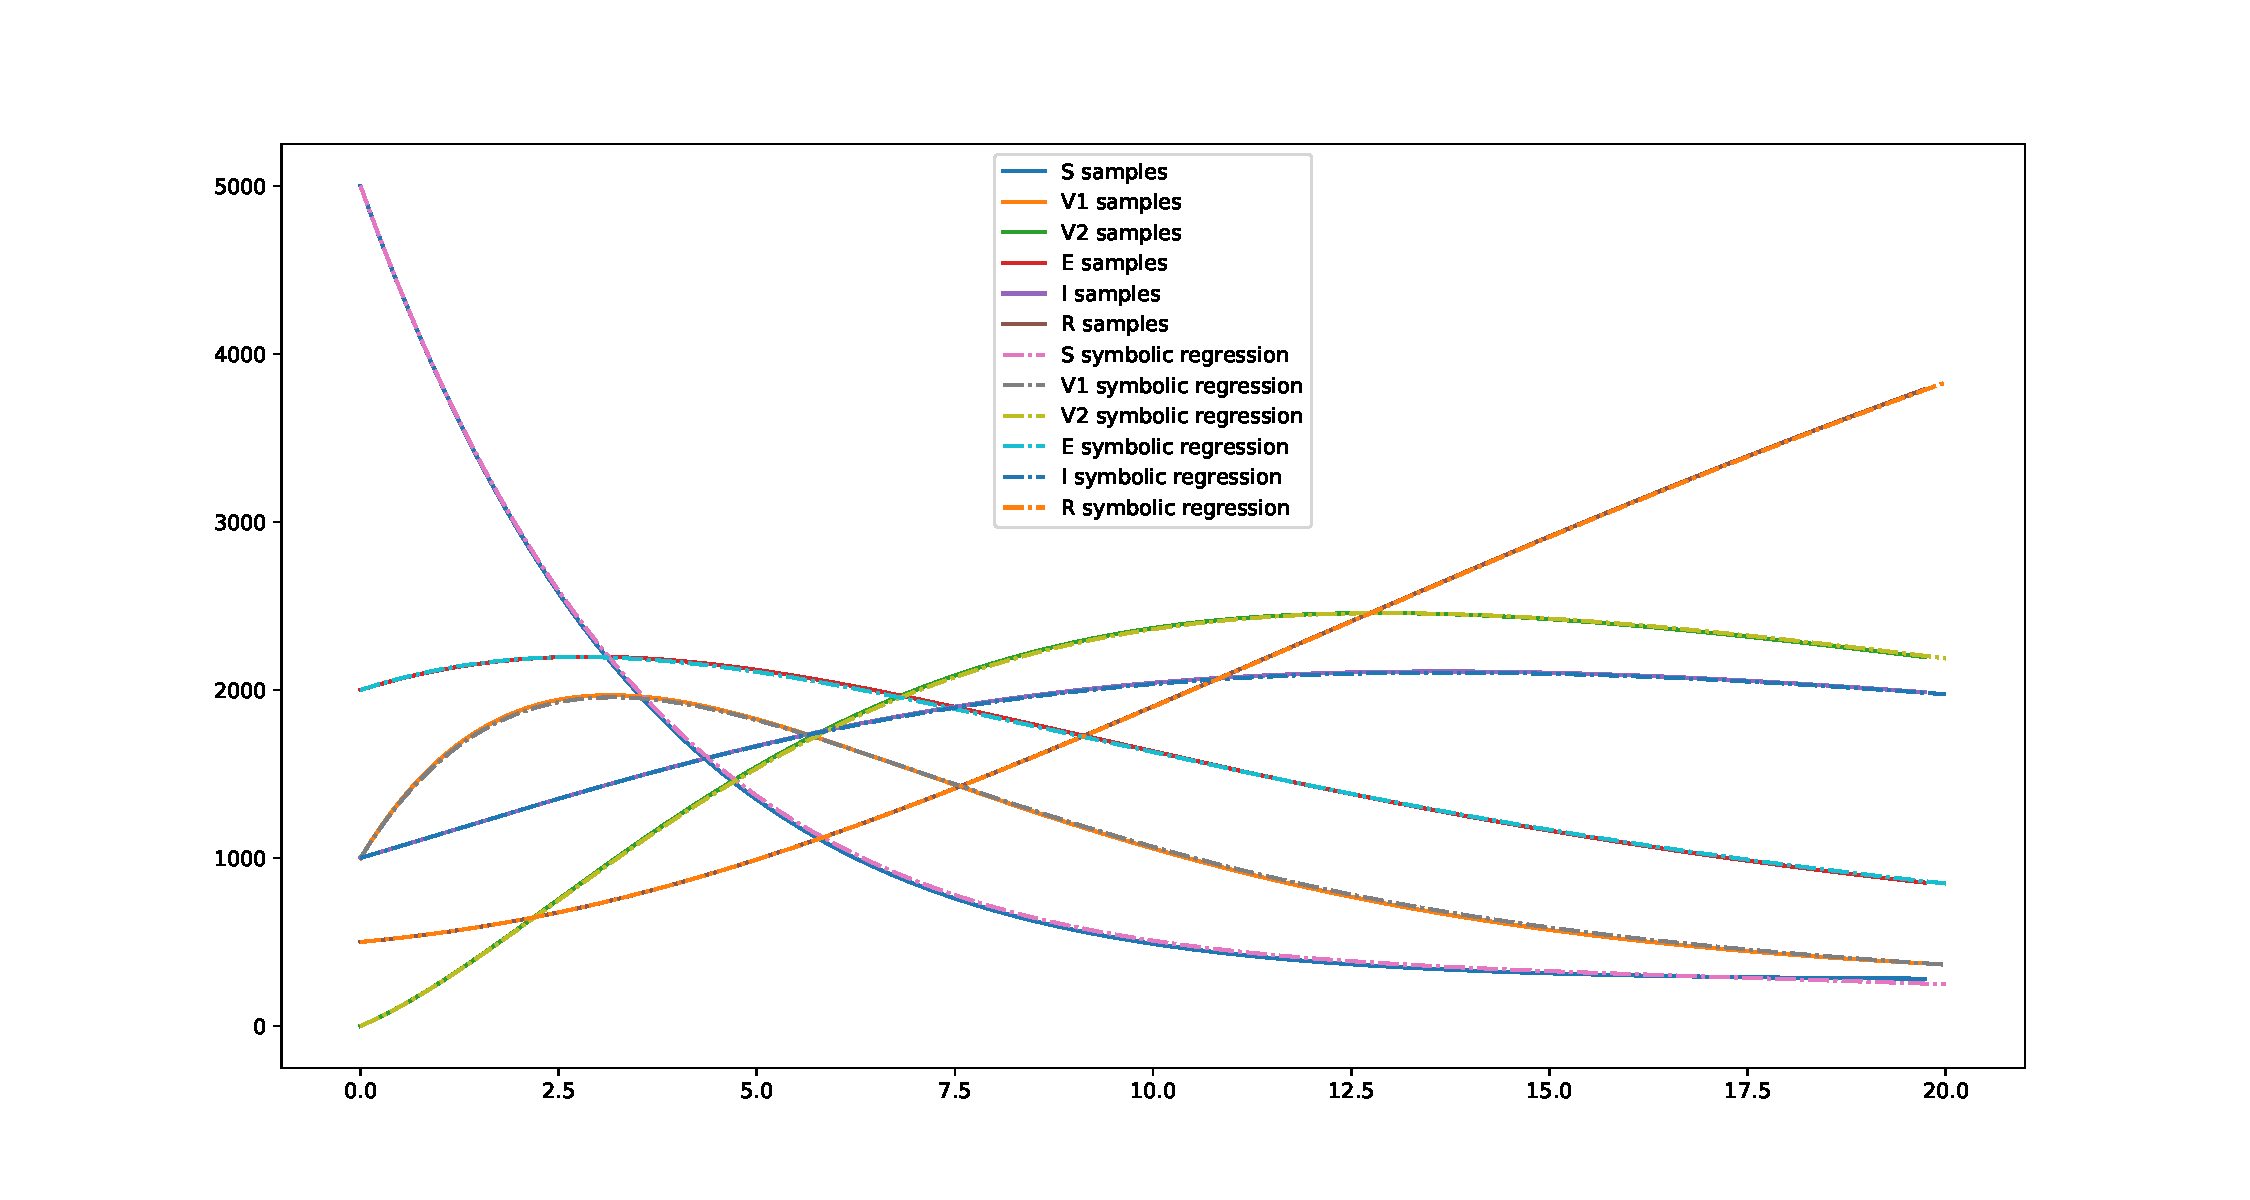
\includegraphics[width=\textwidth]{"figures/final_plot_SVVEIR_0.0.pdf"}
    \begin{align*}
        S' =   & -0.2419 * S -0.02691 * N + 0.15115 * I \\
        V_1' = & -0.21811 * V_1 + 0.19669 * S           \\
        V_2' = & -0.06034 * V_2 + 0.20005 * V_1         \\
        E' =   & 275.33213 * (E / I) -0.19853 * E       \\
        I' =   & -0.0606 * I + 0.09993 * E              \\
        R' =   & -0.01041 * R + 0.05025 * (I + V_2)     \\
    \end{align*}
    \caption{Modelo resultante utilizando datos generados a partir del modelo SVVEIR con ruido máximo de 0\%.}
    \label{fig:final_plot_SVVEIR_0.0}
\end{figure}

\begin{figure}[h]
    \centering
    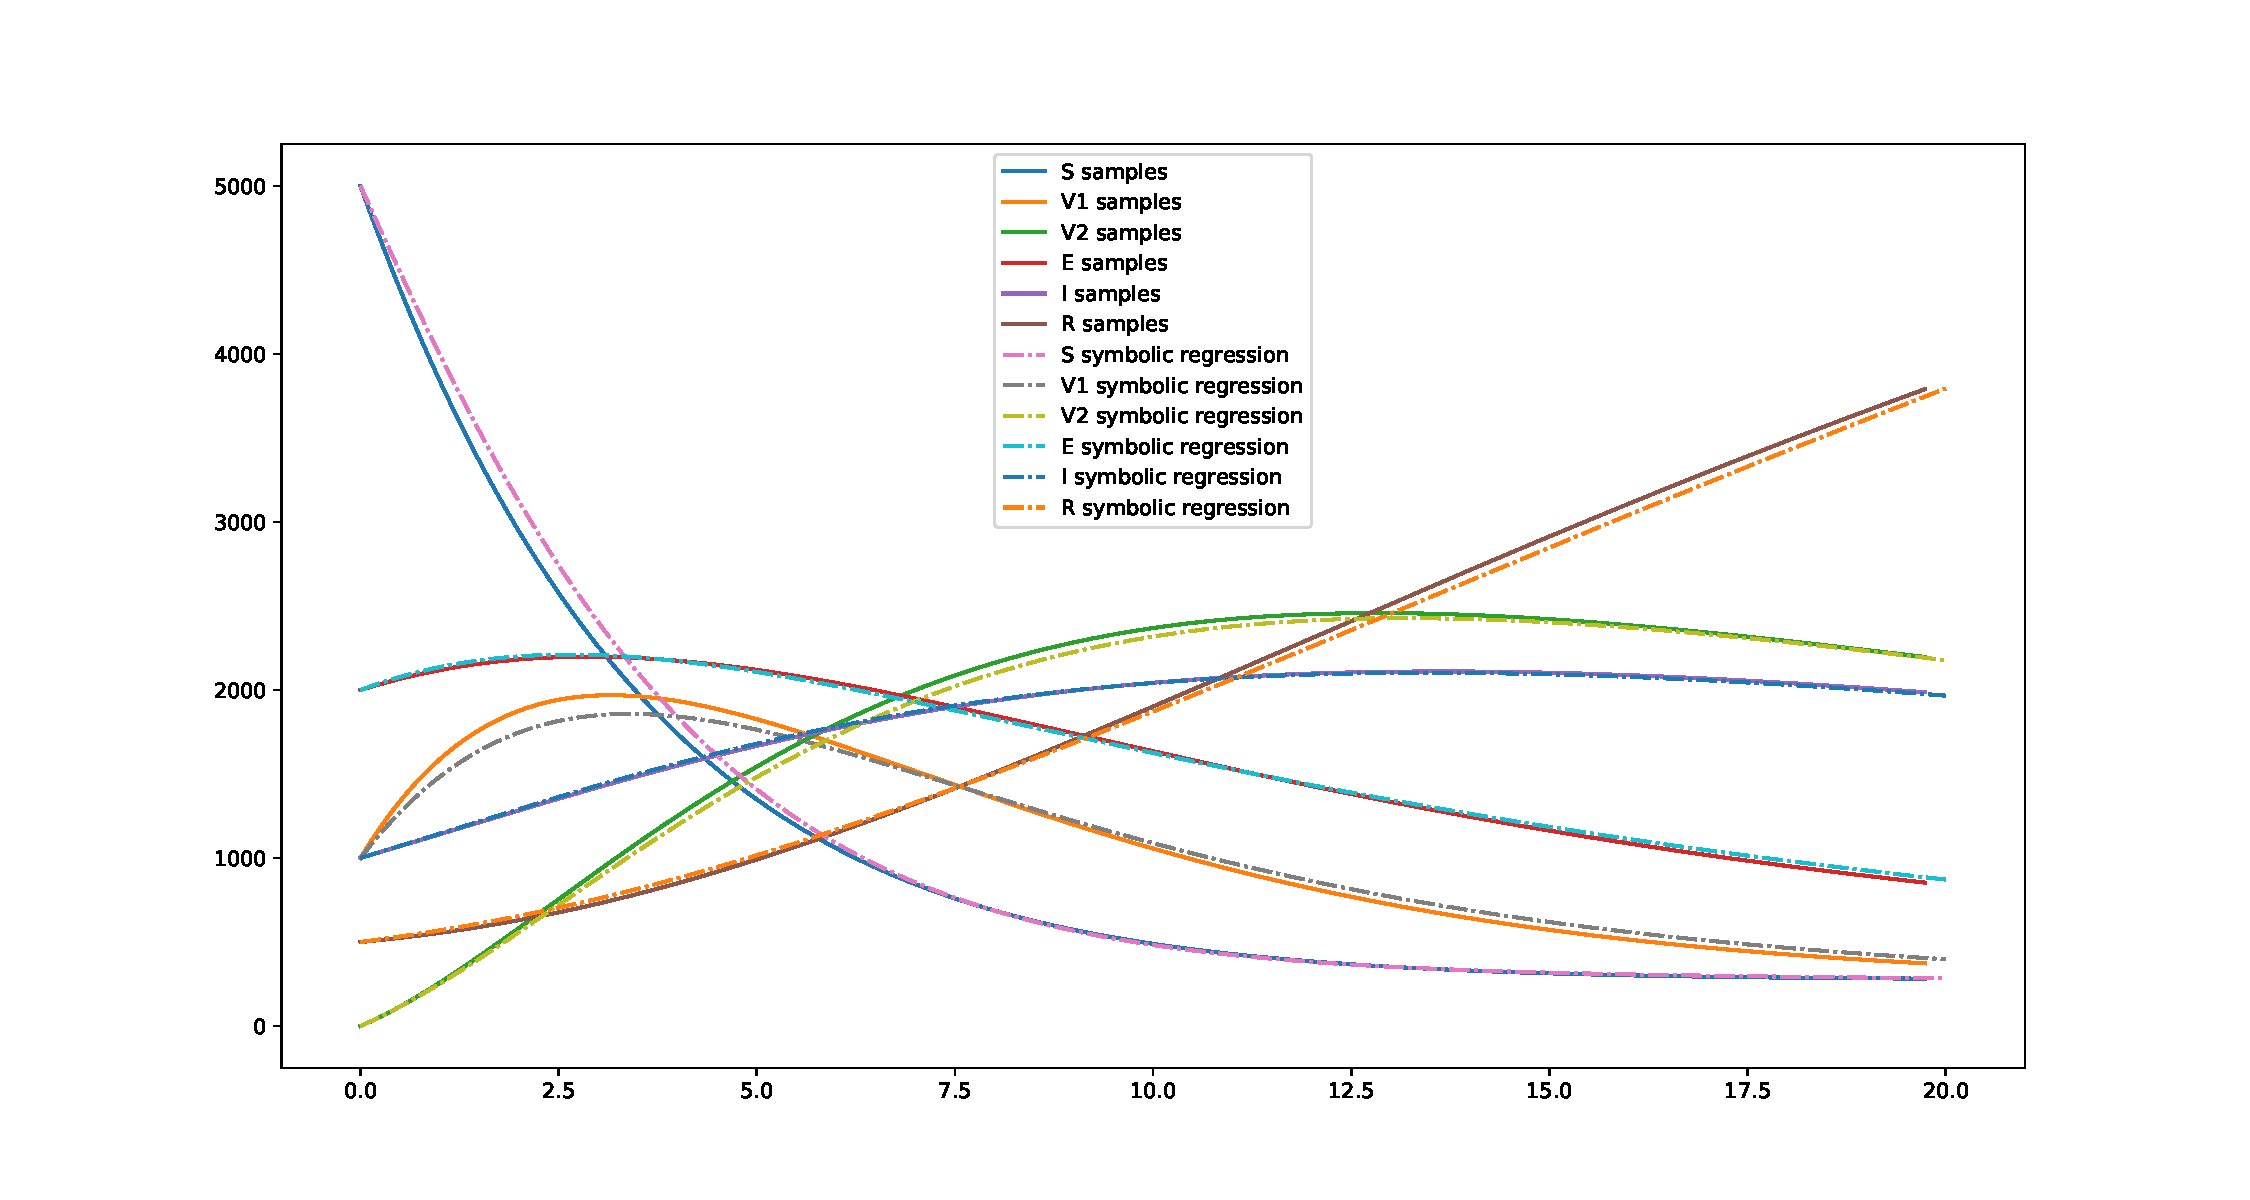
\includegraphics[width=\textwidth]{"figures/final_plot_SVVEIR_0.05.pdf"}
    \begin{align*}
        S' =   & -0.46742 * S + 248.31455 * (S / I) -0.0471 * -I \\
        V_1' = & 0.16019 * S -0.18647 * V1                       \\
        V_2' = & -0.0634 * (V_1 + V_2) + 0.268 * V_1             \\
        E' =   & -0.08141 * E + 0.06799 * S                      \\
        I' =   & -0.06397 * I -0.10318 * -E                      \\
        R' =   & 0.0611 * I + 0.0281 * V_2                       \\
    \end{align*}
    \caption{Modelo resultante utilizando datos generados a partir del modelo SVVEIR con ruido máximo de 5\%.}
    \label{fig:final_plot_SVVEIR_0.05}
\end{figure}

\begin{figure}[h]
    \centering
    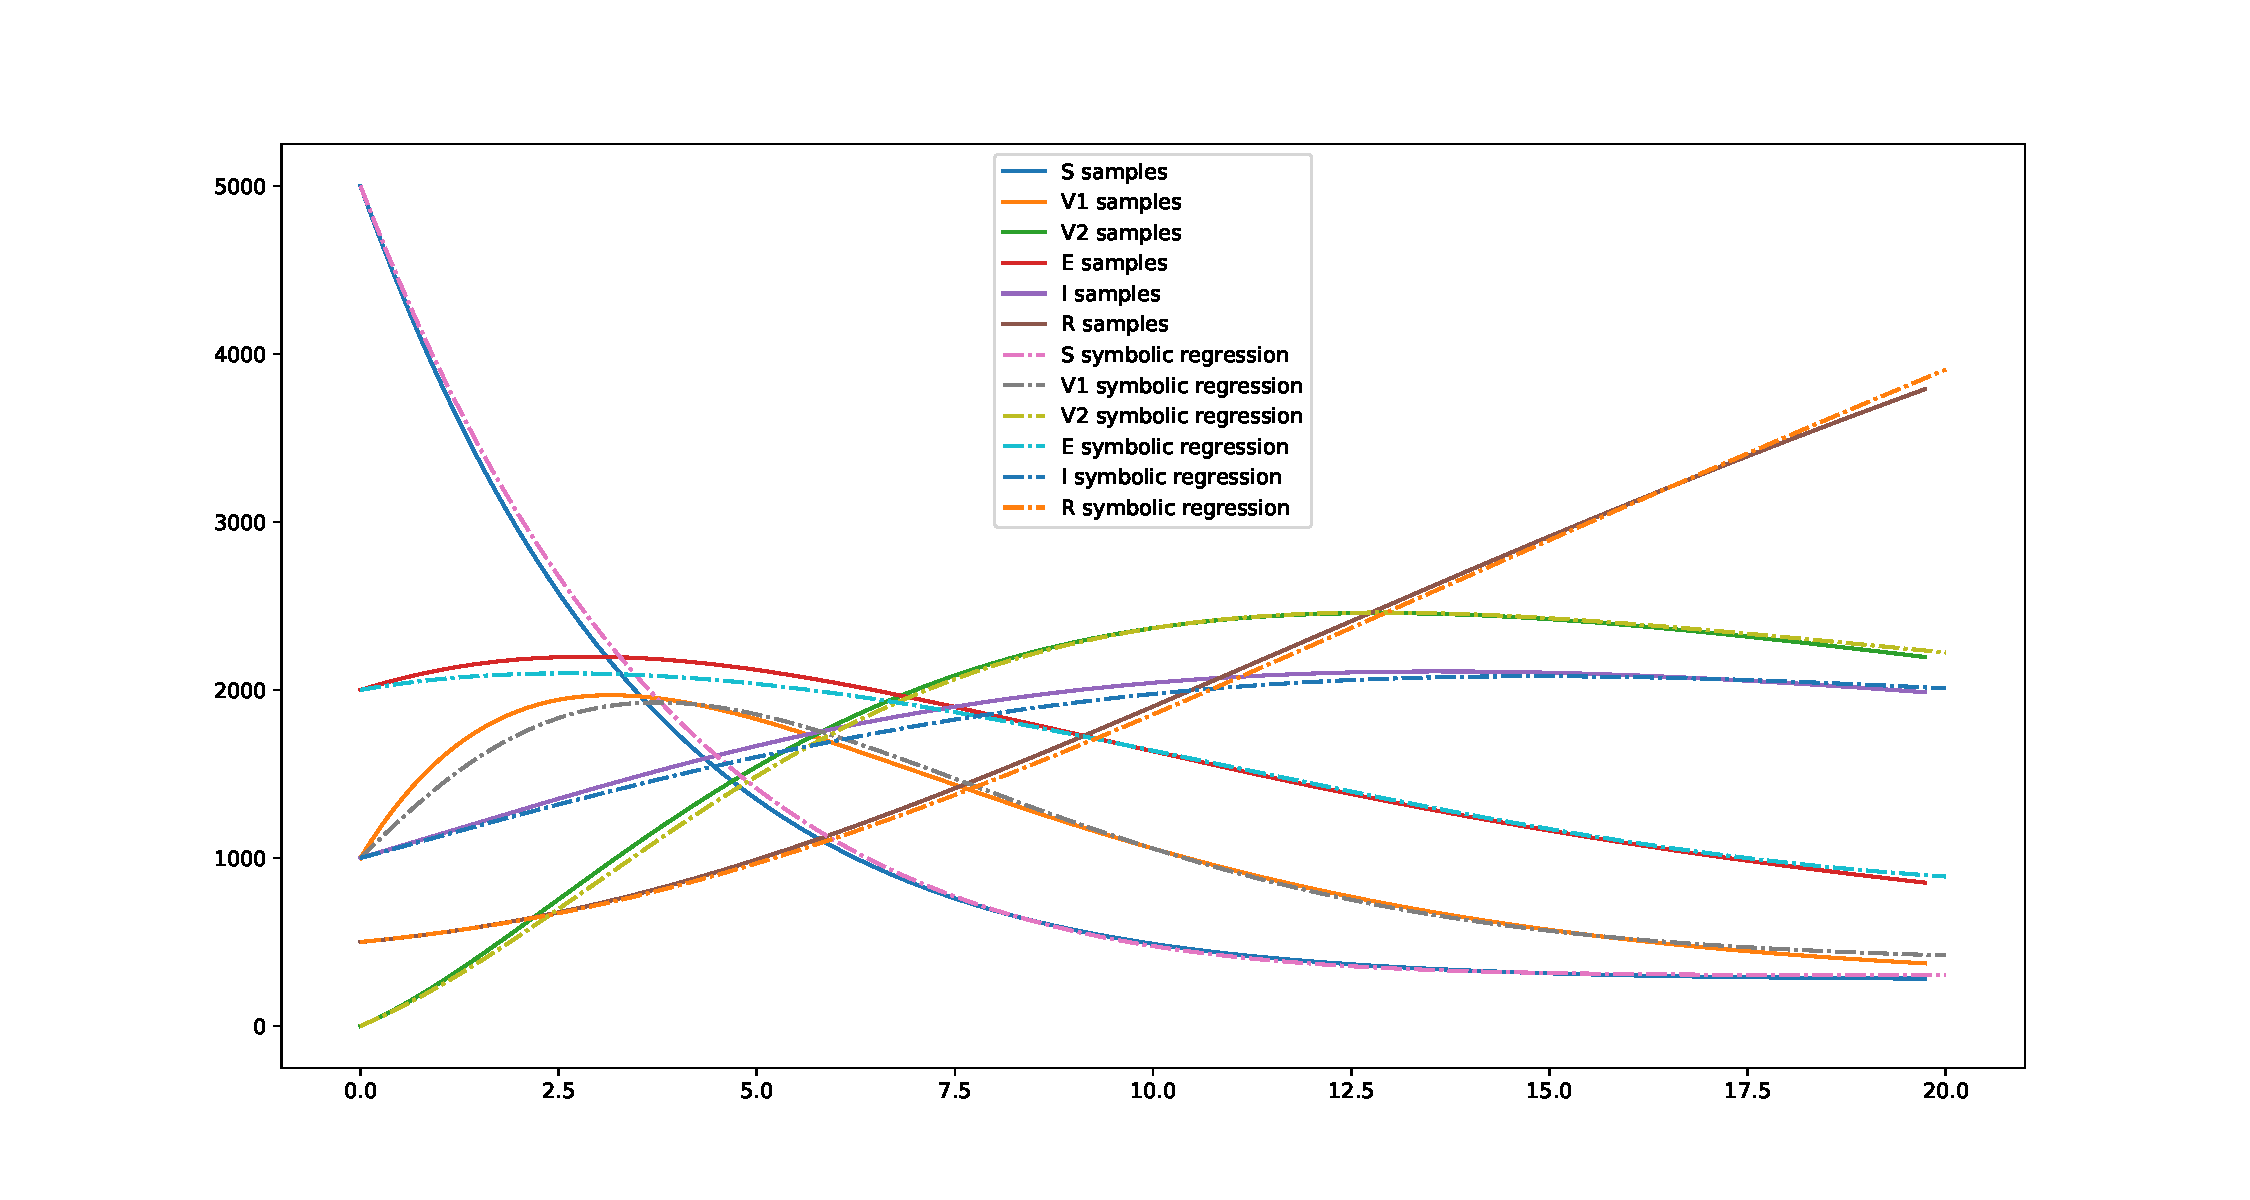
\includegraphics[width=\textwidth]{"figures/final_plot_SVVEIR_0.1.pdf"}
    \begin{align*}
        S' =   & -0.2455 * S + 0.04577 * (I - V_1)       \\
        V_1' = & 0.40625 * S -0.3122 * V_1               \\
        V_2' = & 0.20045 * V_1 -0.05851 * V_2            \\
        E' =   & -0.20957 * I + 0.04696 * N -0.07522 * E \\
        I' =   & 0.09076 * E -0.05165 * I                \\
        R' =   & 0.04626 * (I + V_2)                     \\
    \end{align*}
    \caption{Modelo resultante utilizando datos generados a partir del modelo SVVEIR con ruido máximo de 10\%.}
    \label{fig:final_plot_SVVEIR_0.1}
\end{figure}

Si en lugar de utilizar como aproximación el método de diferencias finitas cuando los datos no poseen ruido, se utiliza el sistema original de SIR, se obtiene que la media del valor de la función de ajuste a lo largo de las 30 ejecuciones del experimento es $3.68731$. El valor máximo de la función de ajuste alcanzado fue de $19.45527$ y el mínimo de $0.58707$, en este último la regresión simbólica no obtuvo el sistema original.

En la siguiente sección se realiza un análisis de los resultados de todos los experimentos realizado.

\section{Análisis de resultados}\label{section:experiments_results}

Los resultados obtenidos durante los experimentos muestran que la regresión simbólica planteada puede encontrar un sistema $f_{aprox}$ que ajuste los datos $y'_{original}$ generados a partir de la derivada aproximada por el método de diferencias finitas sobre los datos $y_{original}$ donde $y_{original}$ son los datos obtenidos de la integración del sistema conocido $f$.

Al generar el conjunto $y_{noise}$ a partir de agregar ruido a $y_{original}$ que describen la función $y$, no se puede aproximar la derivada de $y$ por el método de diferencias finitas. La función $y$ se aproxima utilizando un spline de suavizado cúbico sobre $y_{noise}$ obteniéndose los datos $y_{spline}$. Del spline de suavizado se puede obtener el valor de la primera derivada y así generar el conjunto $y'_{spline}$. Al utilizar los valores de $y_{spline}$ y $y'_{spline}$ en el método de regresión simbólica se obtiene el sistema $f_{aprox_{sr}}$.

El error cuadrático médio de los datos $y_{spline}$ evaluados en el sistema $f_{aprox_{sr}}$ es mayor que el de los datos $y_{original}$ evaluados en el sistema $f_{aprox}$. Mientras mayor el ruido presente en $y_{noise}$ mayor es la diferencia entre los valore del ajuste.

Si se integra el sistema $f_{aprox}$ se obtiene el conjunto de puntos $y_{aprox}$. El valor del error cuadrático medio entre los conjuntos $y_{aprox}$ y $y_{original}$ es menor en los sistemas que no poseen términos con un parámetro sin estar multiplicando una expresión y términos que no poseen una división con una expresión de más de un valor en el divisor.

Si se definen los datos $y_{aprox_{sr}}$ como el resultado de la integración del sistema $f_{aprox_{sr}}$, se puede analizar cómo el error cuadrático medio entre los puntos $y_{aprox_{sr}}$ y $y_{spline}$ es similar al error cuadrático medio entre los puntos $y_{aprox_{sr}}$ y $y_{original}$.

En los sistemas con menos de 6 ecuaciones, los resultados de aplicar la restricción de las variables que pueden existir en cada ecuación no mejoraron los resultados obtenidos sin aplicar la restricción. En el sistema SVVEIR se aprecia una diferencia de hasta 5 veces en el valor de la media del error cuadrático medio entre los valores $y_{aprox_{sr}}$ y $y_{original}$, obteniendose un menor valor del error al aplicar la restricción de las variables que pueden existir en cada ecuación y agregar el valor de $N$ como dato en la regresión simbólica. Por lo que vale la pena restringir las variables que pueden existir en cada ecuación si el modelo que se desea encontrar cuenta con 6 o más ecuaciones.

En los experimentos utilizando los modelos SIR, SIRD, SIQRD y SVVEIR nunca se obtuvo el sistema original como resultado de la regresión simbólica, sin embargo sí se obtuvieron sistemas que fueron capaces de ajustar los datos con valores en la función de ajuste menores que 20.

El uso del modelo original para la aproximación de $y'_{original}$ hace que se obtengan los resultados con el menor valor de ajuste, obtiéndose exactamente el sistema original en algunos experimentos correspondientes a los modelos Lotka-Volterra, SIR, SIRD y SIQRD. Esto no siempre se puede hacer dado que en ocasiones no se conoce el sistema que describen los datos, y hay que aproximar el fenómeno mediante el uso de técnicas como las diferencias finitas o los splines.

El algoritmo de regresión simbólica planteado en este trabajo logra encontrar un sistema de ecuaciones diferenciales lineales con respecto a los parámetros que no presenta advertencias en el momento de su integración utilizando el método \texttt{integrate.odeint} en un $95.18\%$ de los experimentos realizados utilizando como aproximación de la derivada el modelo original. Si se utiliza el método de diferencias finitas como aproximación de la derivada, entonces se encuentran en un $94.81\%$ de los experimentos realizados sin ruido, sistemas que no lanzan advertencias en la integración. Cuando se presentan ruidos máximos de $5\%$ y $10\%$ en los datos, se enucuentran sistemas en un $83.70\%$ y $81.48\%$ de los experimentos, respectivamente.

Dados los experimentos realizados se resalta la dificultad del algoritmo a encontrar sistemas que presenten términos en ecuaciones en los que aparezca un parámetro sin estar acompañado de una expresión. También el algoritmo no encuentra sistemas con valores menores que 20 en la función de ajuste cuando el modelo original que generó los datos presenta términos con divisiones de muchas expresiones en el divisor.

El tiempo que demora el método de regresión simbólica es proporcional a los parámetros que se utilizan en el algoritmo genético y la cantidad de ecuaciones presentes en el sistema. A pesar de qué en todos los experimentos que se realizaron se utilizó un número máximo de 100 generaciones y una población inicial con 100 individuos, la altura máxima de los árboles permitidos para cada modelo y el valor de $MAX\_NODES$ varió. Se puede ver como la media de los tiempos en segundos de los experimentos varía según el modelo seleccionado en la tabla \ref{table:experiments_times} de la página \pageref{table:experiments_times}.

\begin{table}[!h]
    \centering
    \caption{Media de tiempos de ejecución.}
    \begin{tabular}{|c|c|c|c|}
        \hline
                       & \textbf{ruido de 0\%} & \textbf{ruido de 5\%} & \textbf{ruido de 10\%} \\
        \hline
        Lotka-Volterra & 123                   & 123                   & 124                    \\
        \hline
        SIR            & 102                   & 104                   & 105                    \\
        \hline
        SIRD           & 475                   & 482                   & 481                    \\
        \hline
        SIQRD          & 444                   & 448                   & 450                    \\
        \hline
        SVVEIR         & 487                   & 489                   & 488                    \\
        \hline
    \end{tabular}

    \begin{tabular}{|c|c|c|}
        \hline
                       & \textbf{altura máxima permitida} & $MAX\_NODES$ \\
        \hline
        Lotka-Volterra & 10                               & 15           \\
        \hline
        SIR            & 5                                & 20           \\
        \hline
        SIRD           & 10                               & 40           \\
        \hline
        SIQRD          & 10                               & 30           \\
        \hline
        SVVEIR         & 10                               & 30           \\
        \hline
    \end{tabular}
    \label{table:experiments_times}
\end{table}

A continuación se muestran las conclusiones.